%%%%%%%%%%%%%%%%%%%%%%%%%%%%%%%%%%%%%%%%%%%%%%%%%%%%%%%%%%%%%%%%%%%%%%%%%%%%%%%
% SJH-dissertation.tex - version 0.9.1.1 (5/26/2011)
%
% This is based on the template file for the osudiss-2 class. See
% osudiss-2.pdf for documentation, and the GS material 
% for the requirements.
%
% Copy the following osudiss-2 files your latex path (or just the folder containing this file):
% osudiss-2.cls (v0.9.1)
% sa-draftwater.sty
%
% Then, to compile this file:
% latex template
% bibtex template
% latex template
% latex template
%
% (You can also use pdflatex if you prefer.)
%
%%%%%%%%%%%%%%%%%%%%%%%%%%%%%%%%%%%%%%%%%%%%%%%%%%%%%%%%%%%%%%%%%%%%%%%%%%%%%%%
\documentclass[11pt, double, phd]{osudiss-2} 
% The `11pt' option is unnecessary since it is the default

% `onehalf' sets the line spacing to one-and-a-half spacing instead of
% double spacing.

% The `phd' option is unnecessary since it is the default

% Remove `draft' option for final draft

%%%%%%%%%%%%%%%%%%%%%%%%% Packages %%%%%%%%%%%%%%%%%%%%%%%%%
% Load your favorite packages here
\usepackage{graphicx} % for importing images in figures - you definitely want this!
\usepackage{lipsum} % for fake latin text---you probably don't want this
\usepackage{verbatimbox}

% For instance... see osudiss-2.pdf for some suggestions, if you don't
% have a clue
\usepackage{bm} % for bold math---useful
\usepackage{booktabs} % for more professional tables
\usepackage[titletoc]{appendix}

%hyperref packages and options
\usepackage{bookmark} % helps booksmarks look better in PDF
%hypersetup option 'breaklinks' is reguired for line wrapping in the table of contents during latex compilation, and can be removed if you use pdflatex
\hypersetup{colorlinks=true,linkcolor=blue, breaklinks} %internal links in blue, citations in green
%\hypersetup{colorlinks=true,linkcolor=black, citecolor=black, breaklinks} %all links in black
\usepackage[all]{hypcap}

%Use of natbib is STRONGLY recommended to sort and compress your references within each citation
%With these options, natbib will convert i.e. [5,3,9,4] to [3-5, 9]
\usepackage[sort&compress]{natbib}

%required to have latex automatically generate subfigures (i.e. (a), (b) etc)
\usepackage{subfig}
\usepackage[export]{adjustbox}
\setcounter{lofdepth}{2}
\PassOptionsToPackage{obeyspaces}{url}
%\usepackage{hyperref}% http://ctan.org/pkg/hyperref

%load glossaries packages
\usepackage[acronym, section=chapter]{glossaries}
%\usepackage[xindy,acronym, section=chapter]{glossaries} - recommended if supported by your OS
\makeglossaries %required to actually make a glossary
%A list of common acronyms
%Only those used will be displayed, so you can just add to this list
\newacronym{fwhm}{FWHM}{full-width-at-half-maximum}
\newacronym{fft}{FFT}{Fast Fourier Transform}
\newacronym{swpg}{SWPG}{square-wave phase grating}
\newacronym{cats}{CATS}{Complex Attoseond Transient-absorption Spectroscopy}
\newacronym{ir}{IR}{infrared}
\newacronym{doe}{DOE}{diffractive optical element}
\newacronym{hhg}{HHG}{high-harmonic generation}
\newacronym{table}{TABLe}{transition-absorption beamline}
\newacronym{vls}{VLS}{variable line spaced}
\newacronym{mcp}{MCP}{microchannel plate}









 %load list of acronyms contained in acronyms.tex

%The following commands can be used to help deal with "overfull hbox" issues
%See, for example, http://www.tex.ac.uk/cgi-bin/texfaq2html?label=overfull for details
%\pretolerance 1000
\setlength{\emergencystretch}{3em}
%\tolerance 1000

%%%%%%%%%%%%%%%%%%%%%%%%% Custom Commands/Environments %%%%%%%%%%%%%%%%%%%%%%%%%
% Put your favorite custom commands here
%\newcommand{\fish}{\alpha} % some of my students call it the "fish" symbol

%Print list of abbreviations - use same font as List of Figures and List of Tables for the title, and same formatting in the table of contents.
% Argument #1 - title for list of abbreviations (i.e. List of Abbreviations)

\newcommand\PrintListofAbbreviations[1]{
\phantomsection
\addcontentsline{toc}{front}{\typesetColumnHeading{#1}}
\printglossary[type=\acronymtype,title={\protect {\typesetLevelTwo{#1}}}]
}


\newenvironment{chapabstract}{%
    \begin{center}%
      \bfseries Abstract
    \end{center}}%

% Below is an example of customizing the style of headings in your
% dissertation. See osudiss-2.pdf for more information.
%
% For example, if you simply must have uppercase titles:
%\renewcommand\typesetLevelOne[1]{{\Large\textbf{\MakeUppercase{#1}}\par}}
%\renewcommand\typesetLevelTwo[1]{{\Large\textbf{\MakeUppercase{#1}}}}
% Note the \par for \typesetLevelOne
%
% If you want the title to be bold and |\Large| instead of |\Huge|:
%\renewcommand\titleFont{\normalfont\Large\bfseries}

% Add words that TeX may not know how to hyphenate below. This can
% help prevent overfull hboxes. For example,
\hyphenation{eigen-state space-time} 

%%%%%%%%%%%%%%%%%%%%%%%%% Document Metadata %%%%%%%%%%%%%%%%%%%%%%%%%
\title{Complex Attosecond Transient-absorption Spectroscopy}
\author{Stephen J. Hageman}
\advisorname{Louis F. DiMauro}
\degree{Doctor of Philosophy} % Default value
\member{Douglass Schumacher}
\member{Jay Gupta}
\member{Robert Baker}
\authordegrees{M.Sc.}
\graduationyear{2019}
\unit{Graduate Program in Physics} 

%%%%%%%%%%%%%%%%%%%%%%%%% Begin Document %%%%%%%%%%%%%%%%%%%%%%%%%
\begin{document}
\showthe\textwidth
\frontmatter

\begin{abstract}

An experimental technique is developed to measure the complex refractive index in a transient-absorption experiment using attosecond pulse trains.  This complex attosecond transient-absorption spectroscopy (CATS) method is demonstrated by measuring the dynamic change, induced by an infrared dressing pulse, in the real and imaginary parts of the refractive index of the argon $3s3p^6np$ Fano resonances.  Typical attosecond transient-absorption spectroscopy (ATS) measurements only capture the imaginary part of the refractive index, and the real part can only be indirectly calculated.  CATS enables a direct measurement of the real part of the refractive index, and this removes the need to rely upon indirect calculations which are only valid if certain assumptions hold true.  While CATS is demonstrated in a gas phase experiment, it can also be used for condensed matter experiments in either a transmission or reflection geometry.

As a prelude to the demonstration of CATS, an ATS experiment is performed to examine the dynamics of the argon $3s3p^6np$ Fano resonances under the influence of a dressing field.  This ATS measurement reveals a complicated structure of light-induced states and light-induced attenuation in the intensity and time delay dependence of the absorption spectrum.  The theoretical understanding of these features is detailed, and excellent agreement between theoretical and experimental results is demonstrated. 

Additionally, the optical tool that enables CATS to be performed is detailed theoretically and experimentally. This tool is a diffractive optical element known as a $0-\pi$ square-wave phase grating (SWPG).  The SWPG allows for an input femtosecond IR pulse to be duplicated, and the SWPG can control the relative phase between these duplicates.  This relative phase control is demonstrated, and it is used to measure the ground state complex refractive index of silicon and germanium.


\end{abstract}

\dedication{Dedicated to coffee} % Optional, and seriously not this lame
\begin{acknowledgments}

First of all, I would like to thank both my advisor and my emeritus advisor, Lou DiMauro and Pierre Agostini, for all of their support throughout my time in graduate school. I have gotten to work with a wonderful cast of characters during my time in graduate school, and I wouldn't be where I am today without them.

I'd particularly like to acknowledge the friends that I have made while in graduate school: Thuc Mai, Tim Gorman, Alex Dyhdalo, Steve Tjung, Matt Sheffield, Solani Harawa, and Greg Smith.  I truly cherish the time that we have spent together, and I couldn't have asked for a better friend group.  I truly appreciate your friendship, and I know that graduate school would have been a worse experience without you.

I would also like to thank the members of the group that have helped me along the way: Dietrich Kiesewetter, Antoine Camper, Hyunwook Park, Yu Hang Lai, Sha Li, Cosmin Blaga, Kent Talbert, Eric Moore, Kaikai Zhang, Junliang Xu, Abraham Camacho, Sierra O'Bryan, Andrew Piper, Daniel Tuthill, Tim Scarborough, Zhou Wang, Yagou Tang, and Stephen Schoun.  Each and every person in the group has provided invaluable help to me as I navigated my way through research.

I wouldn't have made it through graduate school without the help of machinists Mike Graham and Pete Gosser.  They are truly the ones who deserve credit for the TABLe.  They went above and beyond to help Greg and me when we were designing it, and it was awesome to work with them on such a large project.

It is important that I acknowledge the contributions of my parents and my sister: Jim, Beth, and Jennifer Hageman.  They have provided endless support to me, and they have helped shape the person I am today.  They have always encouraged me to follow my passions, and I will be eternally grateful for that.

I would also like to thank Wallace and Ricky Hageman.  They have been by my side throughout graduate school, and they have always been there when I needed some support. They inspired some of the acronyms used throughout this dissertation.

Finally, I would like to thank Rileigh.  Without graduate school, I wouldn't have met her, and without her, graduate school wouldn't have been the same.  Her belief in me helped carry me through some dark days, and I am eternally grateful that she is by my side.


%I would like to thank Sir Rickenabcker First of His Name, Last of His Kind, for his eternal indifference.


\end{acknowledgments}
\begin{vita}
%\dateitem{Oct 17, 1990}{Born---Kolkata, India}
\dateitem{2011}{Bachelors of Science in Physics and Mathematics, Johns Hopkins University}

\dateitem{2014}{Master of Science in Physics, The Ohio State University}
\dateitem{2014 to present}{Graduate Research Associate, The Ohio State University}
% Insert other relevant items here (GTA, etc.)

\begin{publist}

\pubitem{Vyacheslav E. Leshchenko, Bradford K. Talbert, Yu Hang Lai, Sha Li, Yagou Tang, \textbf{Stephen J. Hageman}, Greg Smith, Pierre Agostini, Louis F. DiMauro, and Cosmin I. Blaga. ``Cr:ZnSe mid-IR, multi-mJ, few-cycle amplifier: a new platform for attosecond soft-X-ray physics," Optica 7 (8), 981-988 (2020)}

\pubitem{Antoine Camper, Hyunwook Park, \textbf{Stephen J. Hageman}, Greg Smith, Thierry Auguste,
	Pierre Agostini, and Louis F. DiMauro. ``High relative-phase precision beam duplicator
	for mid-infrared femtosecond pulses." Optics Letters, 44 (22), 5465-5468 (2019)}

\pubitem{B. Peters, A. Alfonsov, C. G. F. Blum,\textbf{ S. J. Hageman}, P. M. Woodward, S. Wurmehl, B. Büchner, and F. Y. Yang, ``Epitaxial films of Heusler compound Co$_{2}$FeAl$_{0.5}$Si$_{0.5}$ with high crystalline quality grown by off-axis sputtering,” Appl. Phys. Lett. 103, 162404 (2013)}
\pubitem{W. G. Wang, A. Pearse, M. Li, \textbf{S. Hageman}, A. X. Chen, F. Q. Zhu, and C. L. Chien, ``Parallel fabrication of magnetic tunnel junction nanopillars by nanosphere lithography,” Scientific Report 3, 1948 (2013)}
\pubitem{W. G. Wang, M. Li, \textbf{S. Hageman}, and C. L. Chien, "Electric-field-assisted switching in magnetic tunnel junctions," Nature Mater. 11, 64 (2012)}
\pubitem{W. G. Wang, \textbf{S. Hageman}, M. Li, S. X. Huang, X. M. Kou, X. Fan, J. Q. Xiao, and C. L. Chien, ``Thermal annealing study of magnetoresistance and perpendicular anisotropy in magnetic tunnel junctions based on MgO and CoFeB," Appl. Phys. Lett. 99, 102502 (2011)}


\end{publist}


\begin{fieldsstudy}
\majorfield{Physics}
%\onestudy{Particle Astrophysics}{Connolly group} % optional
% Alternatively you can do:
\end{fieldsstudy}

\end{vita}

\tableofcontents 

% list of figures (comment out if you don't have any figures)
\clearpage %remove if you don't want a page break before list of figures
\listoffigures 

% list of tables (comment out if you don't have any tables)
%\clearpage  %remove if you don't want a page break before list of tables
%\listoftables 

%print glossary - comment out if you don't want this.  Make sure you also add \glsdisablehyper if you don't want to print a glossary, but do use the %glossaries package to keep track of acronyms
\clearpage %remove if you don't want a page break before list of abbreviations
\PrintListofAbbreviations{List of Abbreviations} %Title is in { } - change if desired
\printglossary[type=\acronymtype]

\mainmatter
%\chapter{Introduction}
\label{Intro}

\section{HHG}
\label{intro_HHG}

A common difficulty in working with extreme ultraviolet (XUV) light is the lack of efficient and broadband optics, especially beam splitters. Here, we introduce a method for generating two sources of XUV light by high harmonic generation using a phase grating.  This phase grating allows for precise and stable control of the phase delay between the two generate XUV beams.  This can be thought of as an inline interferometer, and it can have applications for XUV Fourier transform spectroscopy , as well as transient absorption spectroscopy.

\section{Theory}
\label{theory_ts}

In order to generate two ostensibly identical XUV pulses, we take advantage of a diffractive optical element known as a beam splitting grating.   The idea is to introduce a periodic phase step in the beam, which will cause the beam to diffract into different orders.  The phase step is designed such that the +1 and -1 orders are most efficiently populated, with an efficiency of up to 81$\%$.  These will be used to generate spatially separated harmonics.

A key advantage to this method is that it allows for control of the relative phase between the two sources generating harmonics.  By translating the grating relative to the beam, the relative phase difference between the +1 and -1 orders goes from -2$\pi$ to 2$\pi$.  This can be seen in the phase of the electric field at the focus:



\chapter{Two-source high harmonic generation}
\label{two_source}

\section{Introduction}
\label{intro_ts}

A common difficulty in working with extreme ultraviolet (XUV) light is the lack of efficient and broadband optics, especially beam splitters. Here, we introduce a method for generating two sources of XUV light by high harmonic generation using a phase grating.  This phase grating allows for precise and stable control of the phase delay between the two generate XUV beams.  This can be thought of as an inline interferometer, and it can have applications for XUV Fourier transform spectroscopy, as well as transient absorption spectroscopy.

\section{Theory}
\label{theory_ts}

In order to generate two ostensibly identical XUV pulses, we take advantage of a diffractive optical element known as a beam splitting grating.   The idea is to introduce a periodic phase step in the beam, which will cause the beam to diffract into different orders.  The phase step is designed such that the +1 and -1 orders are most efficiently populated, with an efficiency of up to 81$\%$.  These will be used to generate spatially separated harmonics.

A key advantage to this method is that it allows for control of the relative phase between the two sources generating harmonics.  By translating the grating relative to the beam, the relative phase difference between the +1 and -1 orders goes from -2$\pi$ to 2$\pi$.  This can be seen in the phase of the electric field at the focus:

\begin{equation}\label{eq:field}
	S(x) = \sum_{n} E(x - x_{n})
\end{equation}

\begin{figure}
	\centering
	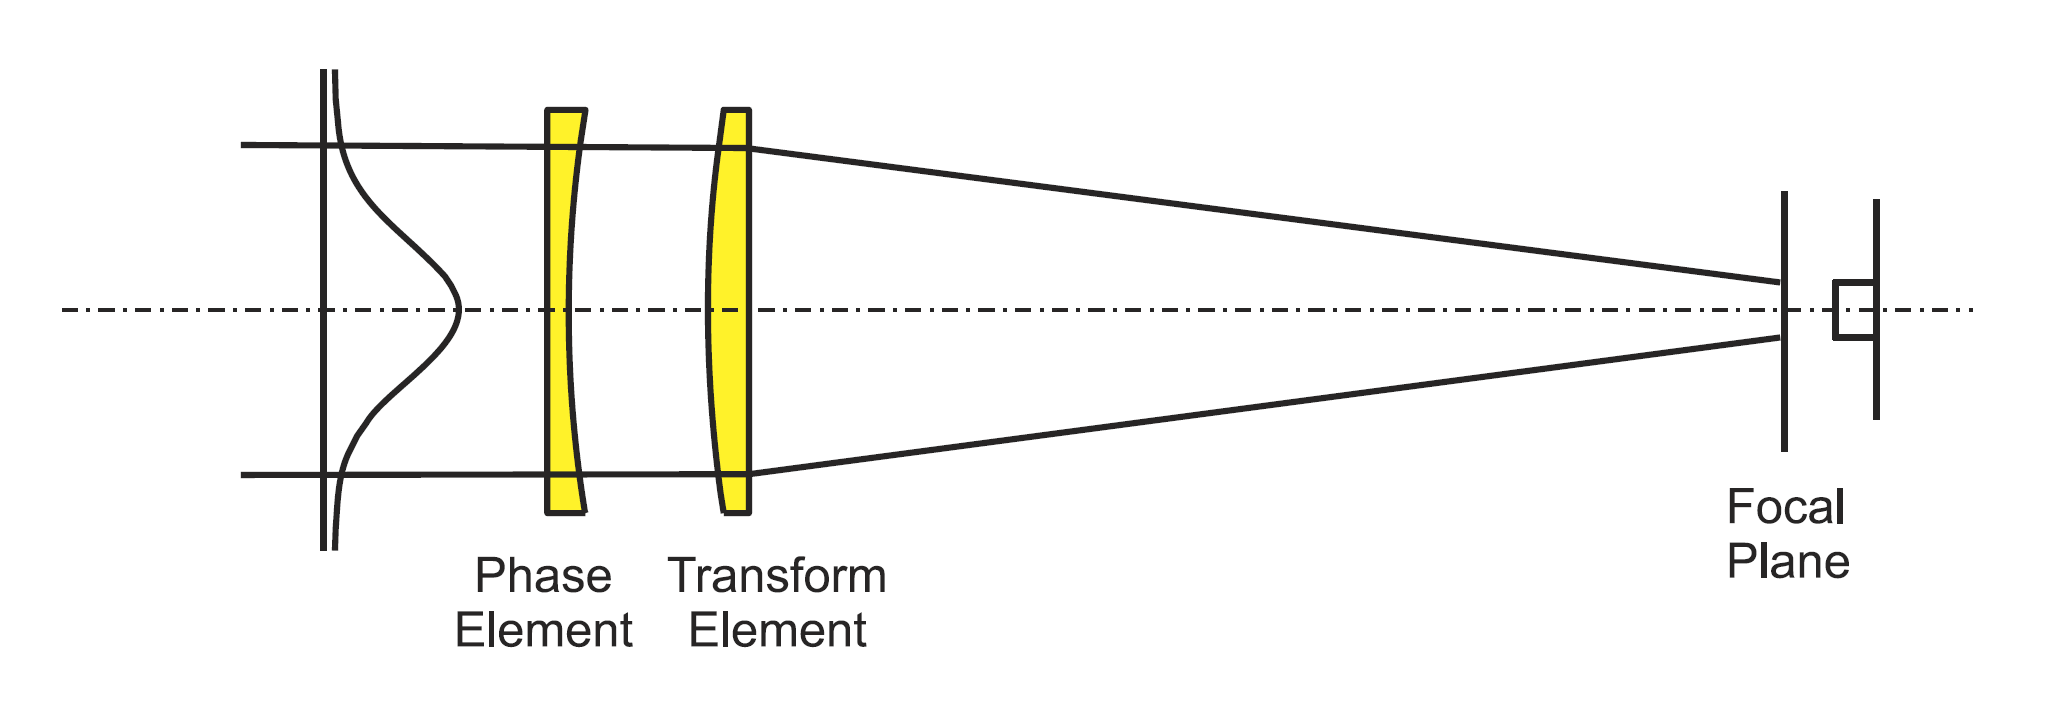
\includegraphics[width=0.9\textwidth]{figures/Two_source/romero_beam_shaping_schematic.png}
	\caption{Schematic demonstrating how to use a diffractive optical element to shape the beam profile at the focal plane. A collimated coherent beam is incident upon a diffractive optical element which shapes the phase of the incident beam, and then a lens is as a transform element to Fourier transform the beam at the focal plane.  The intensity profile at the focal plane can be controlled by altering the spatial dependence of the phase imparted upon the incident beam by the phase element. Adapted from \cite{romero_mathematical_2010-1}}
	\label{fourier_beam_shaping_scheme}
\end{figure}

\begin{figure}
	\centering
	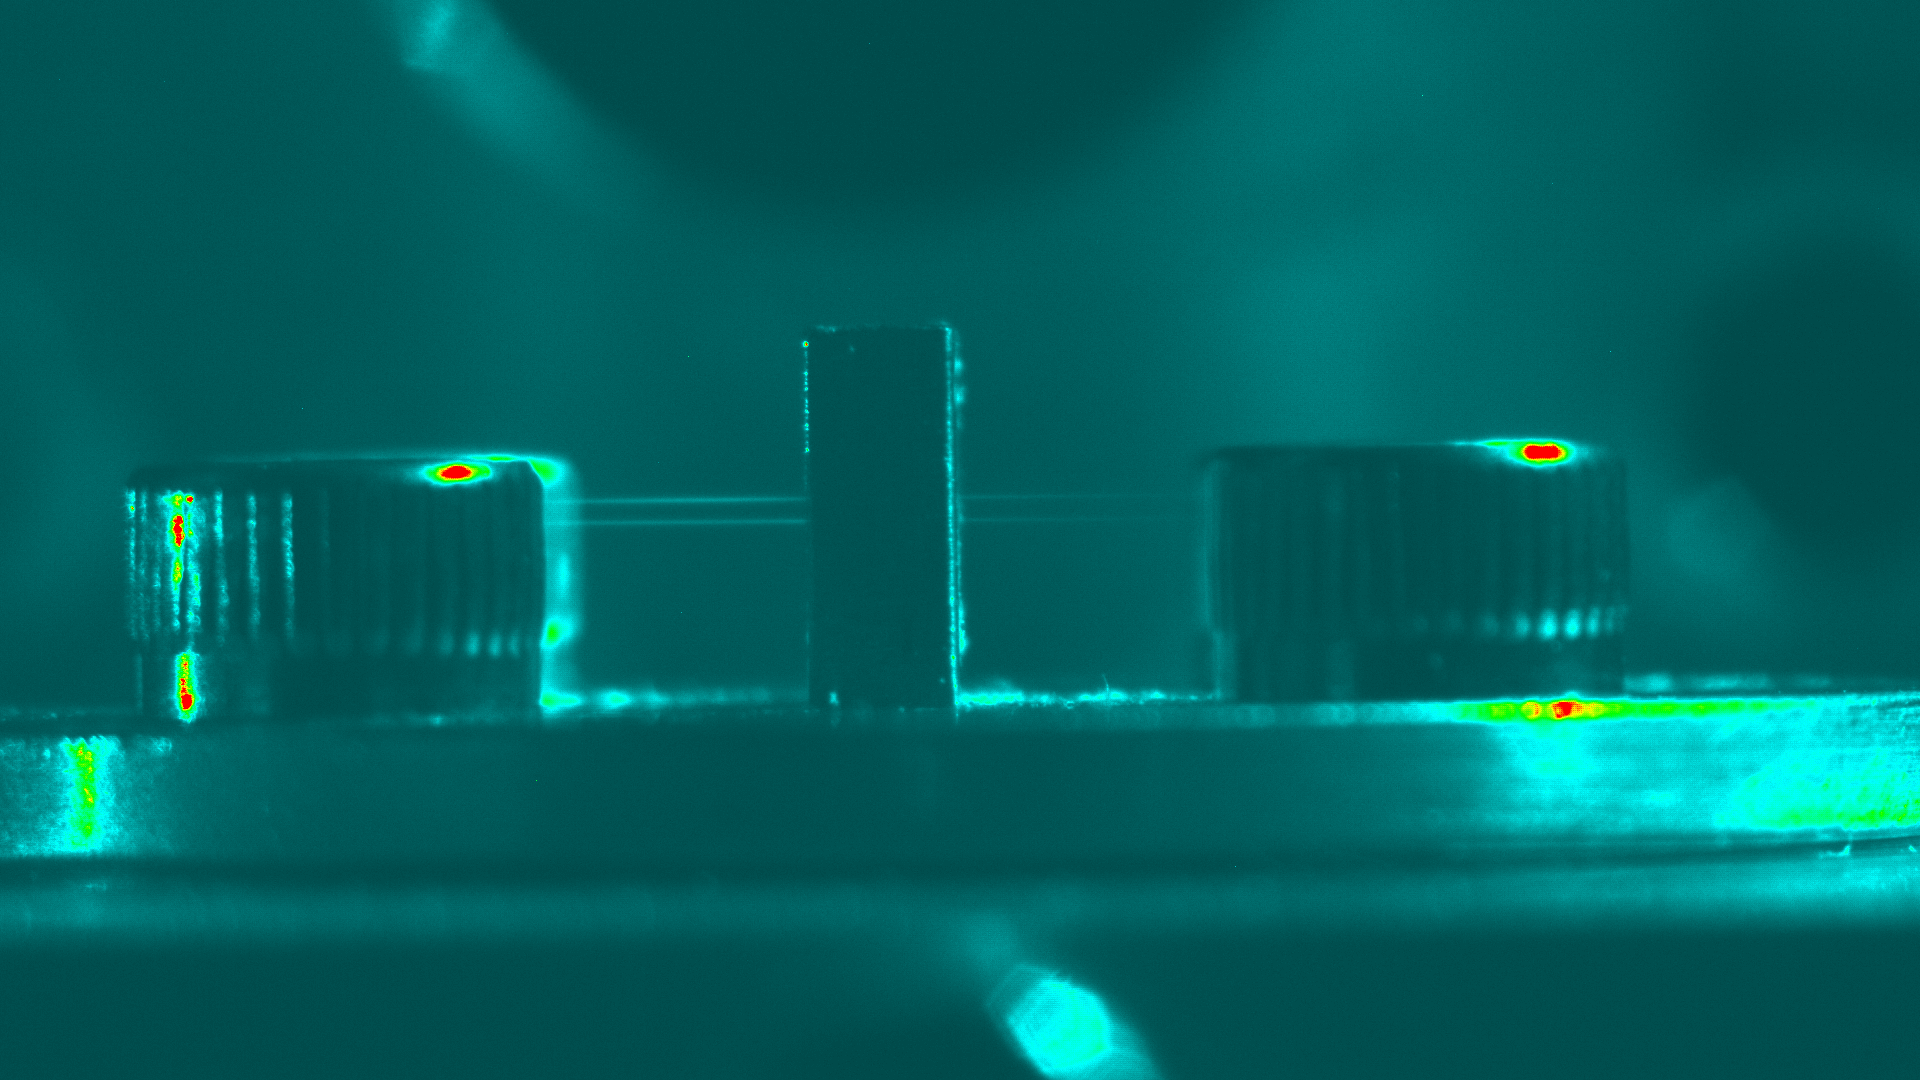
\includegraphics[width=0.9\textwidth]{figures/Two_source/ts_filament_gas_cell.png}
	\caption{Camera image of two sources generating a filament in a gas cell. Image was taken while chamber was vented and at ambient pressure.}
	\label{ts_filament}
\end{figure}

%\lipsum

\begin{figure}
	\centering
	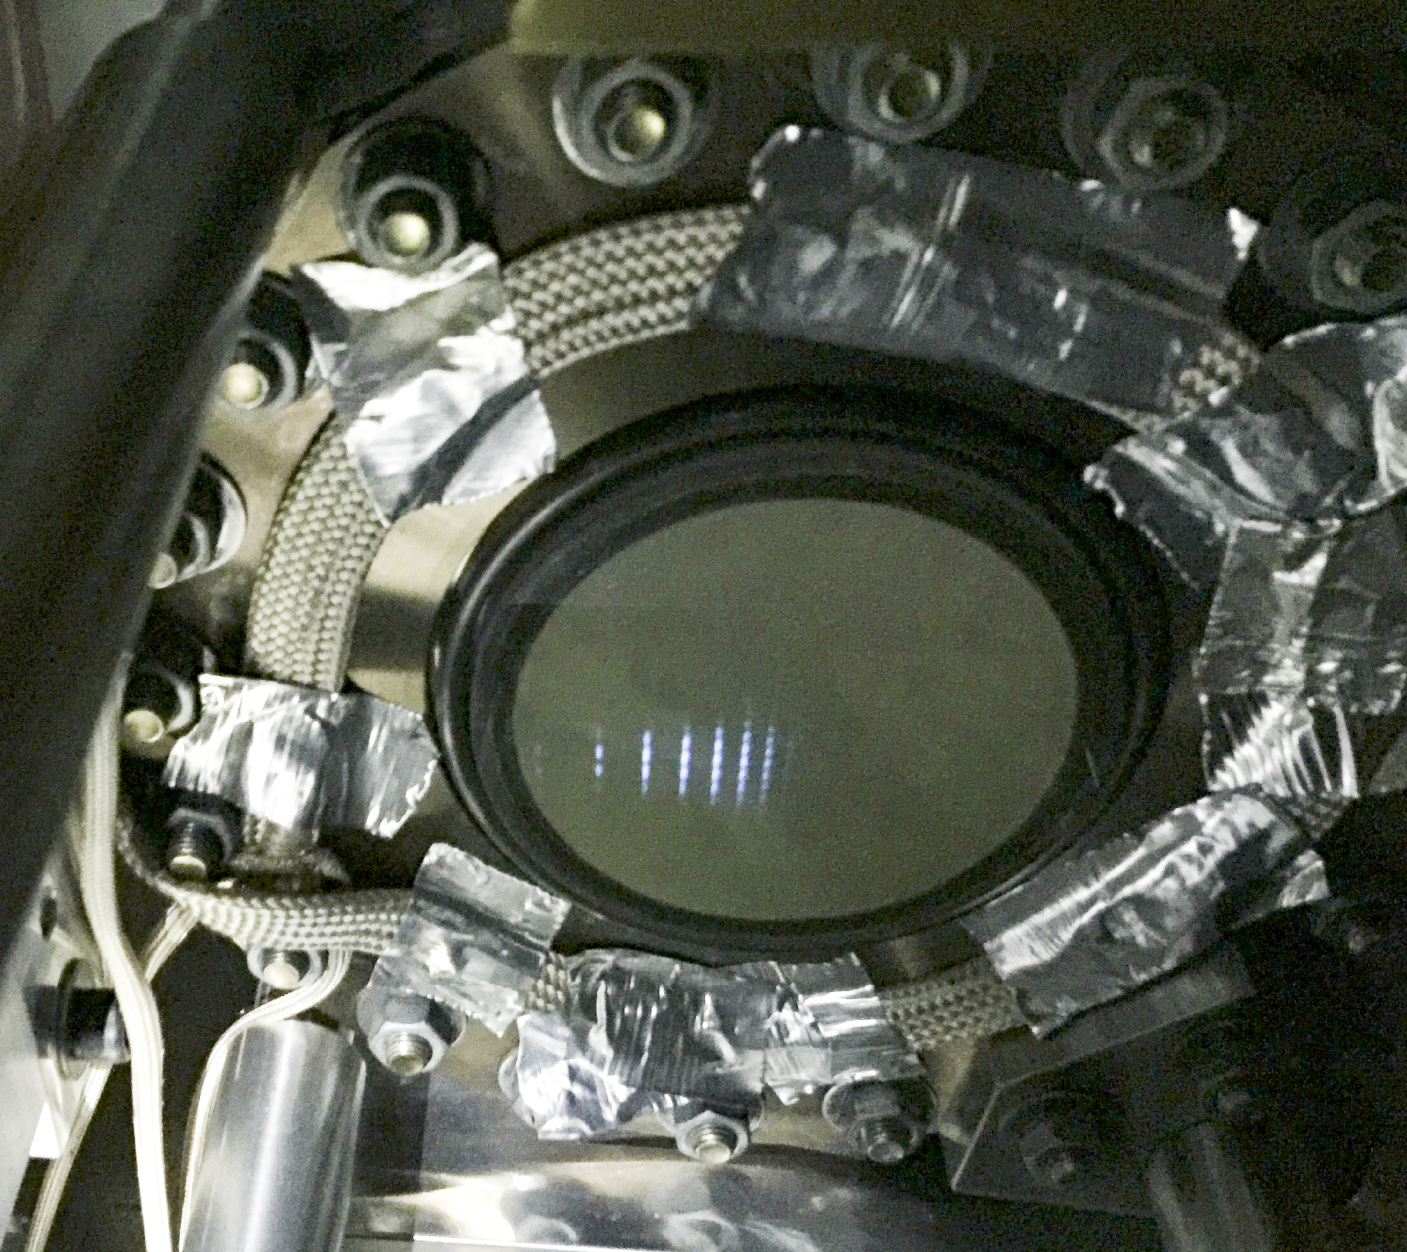
\includegraphics[width=0.9\textwidth]{figures/Two_source/MCP_ts_harmonics.png}
	\caption{Camera image of the output of the phosphor screen.  Harmonics are visible by eye.}
	\label{MCP_ts_harmonics}
\end{figure}


%\lipsum
%\chapter{Theory of attosecond transient absorption}
\label{atas_theory}

\section{Introduction}
\label{intro_atas_theory}

A common difficulty in working with extreme ultraviolet (XUV) light is the lack of efficient and broadband optics, especially beam splitters. Here, we introduce a method for generating two sources of XUV light by high harmonic generation using a phase grating.  This phase grating allows for precise and stable control of the phase delay between the two generate XUV beams.  This can be thought of as an inline interferometer, and it can have applications for XUV Fourier transform spectroscopy, as well as transient absorption spectroscopy \cite{diffuse}.

\section{Theory}
\label{theory_ts}

In order to generate two ostensibly identical XUV pulses, we take advantage of a diffractive optical element known as a beam splitting grating.   The idea is to introduce a periodic phase step in the beam, which will cause the beam to diffract into different orders.  The phase step is designed such that the +1 and -1 orders are most efficiently populated, with an efficiency of up to 81$\%$.  These will be used to generate spatially separated harmonics.

A key advantage to this method is that it allows for control of the relative phase between the two sources generating harmonics.  By translating the grating relative to the beam, the relative phase difference between the +1 and -1 orders goes from -2$\pi$ to 2$\pi$.  This can be seen in the phase of the electric field at the focus:





%\chapter{Transient Absorption Beamline}
\label{chap:beamline}

\section{Introduction}
\label{intro_beamline}
In order to perform the experiments described in this dissertation, it was necessary to construct a purpose-built experimental apparatus, and this is what will be referred to as the Transient Absorption Beamline (TABLe).  The TABLe was designed, constructed, and commissioned with the express intent to perform attosecond transient absorption experiments in the XUV energy range using a HHG source.  The TABLe was designed, constructed, and commissioned by my fellow graduate student, Greg Smith, and myself. Each of us took responsibility for certain design aspects.  My contributions to the design and capabilities of this beamline is discussed within this Chapter, and further details can be found in Greg Smith's dissertation \cite{smithApplicationAttosecondTechniques2020}.

\section{Laser System}
\label{sec:laser_system}
To begin, it is important to describe the laser system that was used for all of the experiments described in this dissertation.  This laser system in question is a commercial system from Spectra-Physics called the Spitfire Ace PA.  It is a titanium-doped sapphire (Ti:Sapph) laser that is based on chirped-pulse amplification (CPA).\footnote{The development of the CPA laser system by Gérard Mourou and Donna Strickland was awarded the Nobel Prize in 2018.}  A schematic of this CPA system is shown in figure \ref{fig:CPA}.  The first main component is the oscillator, and this is a laser cavity that is designed to produce pulses via mode-locking.  In the Spitfire, this oscillator is acousto-optic mode-locked, and it produces pulses of 10 nJ at repetition rate of 80 MHz with a bandwidth of 25 nm centered at 800 nm.  The next component is a stretcher, which is used to reduce the peak intensity of each pulse before amplification to avoid damaging optics.  Following the stretcher, the next component is the regenerative amplifier (regen).  The regen is a cavity-based amplifier that uses a Pockels cell as a pulse picker to allow a single oscillator pulse into the cavity to be amplified.  The pulse is kept in the cavity for a set number of round trips before it is released, and at this point the pulse is now at the mJ level of pulse energy.  Following this stage of amplification, another stage is required to further amplify the pulse energy, and this is accomplished using single-pass amplifier.  For the Spitfire system, the energy after these amplification stages is 15 mJ at a repetition rate of 1 kHz, however the pulse is still stretched in time.  So, the last component is the compressor, and this uses a diffraction grating to compress the pulse down to the final pulse duration.  After all of these stage, the Spitfire is capable of outputting pulses with a pulse duration of 60 fs and a pulse energy of 12 mJ with a repetition rate of 1 kHz.

\begin{figure}
	\centering
	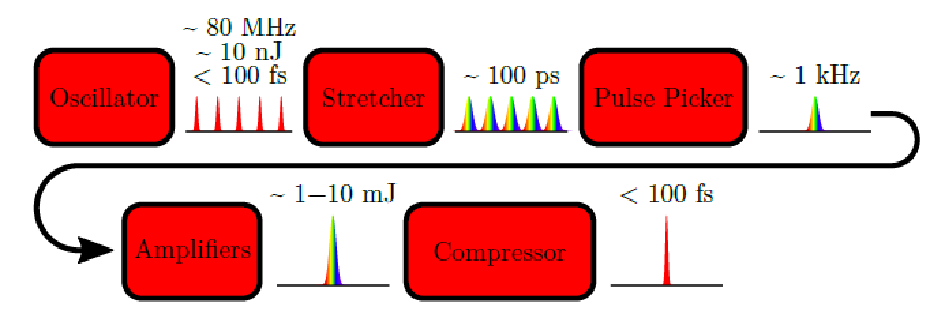
\includegraphics[width=1.0\textwidth]{figures/Beamline/CPA.pdf}
	\caption[Schematic of a CPA laser system]{Schematic of a CPA laser system. Adapted from \cite{kiesewetterDynamicsNearThresholdAttosecond2019}. }
	\label{fig:CPA}
\end{figure}

Many experiments can be done using these 800 nm pulses, however for the experiments described herein, wavelengths longer than 800 nm are required.  To  accomplish this, an optical parametric amplifier (OPA) is used to convert the 800 nm pulses into longer wavelengths, and this allows for wavelength tunability.  The basic idea of the OPA is to use nonlinear media to convert one larger photon (800 nm pump) into two smaller photons (1200-1600 nm signal and 1600-2400 nm idler) \cite{boydNonlinearOptics2008}.  The OPA used with the Spitfire is a commercial HE-TOPAS Prime from Light-Conversion.  The basic optical layout is shown in figure \ref{fig:OPA}, and consists of an initial white-light continuum generation followed by a series of nonlinear Beta Barium Borate (BBO) crystals.  These BBO crystals are optimized for difference frequency generation to amplify the 1200-1600 nm signal.  After these stages of amplification, the TOPAS can output a combine energy of 6 mJ for the combined signal and idler beams.  The pulse duration of these pulse can vary depending upon alignment and the wavelength selected, however it is generally around 60 fs. An example of a typical pulse in both intensity and spectrum is shown in figure \ref{fig:TOPAS_FROG}.  This was measured using a standard second-harmonic generation FROG setup which allows for full characterization of the pulse by extracting both the spectral amplitude and phase \cite{trebinoFrequencyresolvedOpticalGating2000}.

\begin{figure}
	\centering
	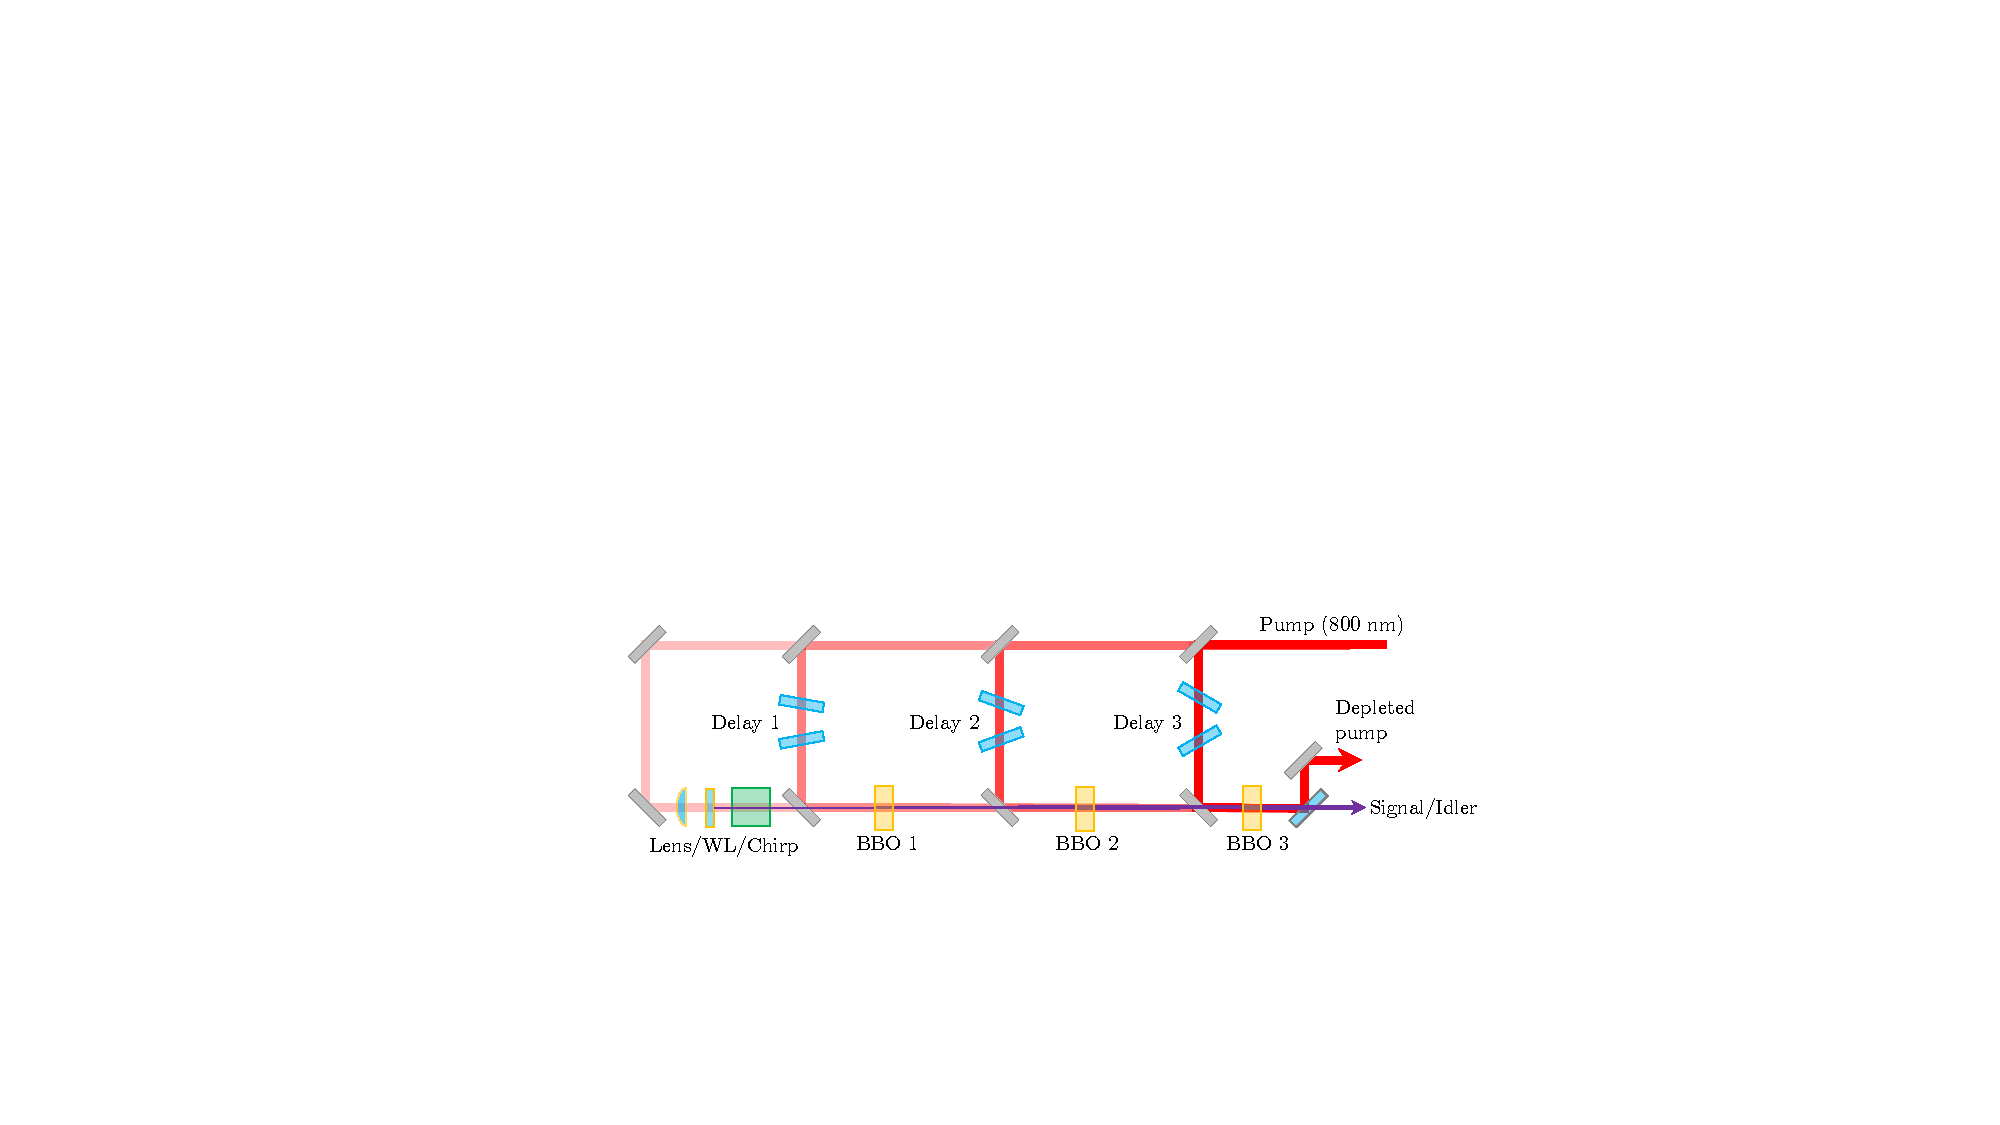
\includegraphics[width=1.0\textwidth]{figures/Beamline/OPA.pdf}
	\caption[Schematic of TOPAS]{Schematic of TOPAS OPA.  The pump beam enters with a pulse energy of 12 mJ before being split three times.  The lowest pulse energy beam is used to generate white light that is used to seed difference frequency generation in the successive BBO crystals.}
	\label{fig:OPA}
\end{figure}
\begin{figure}
	\centering
	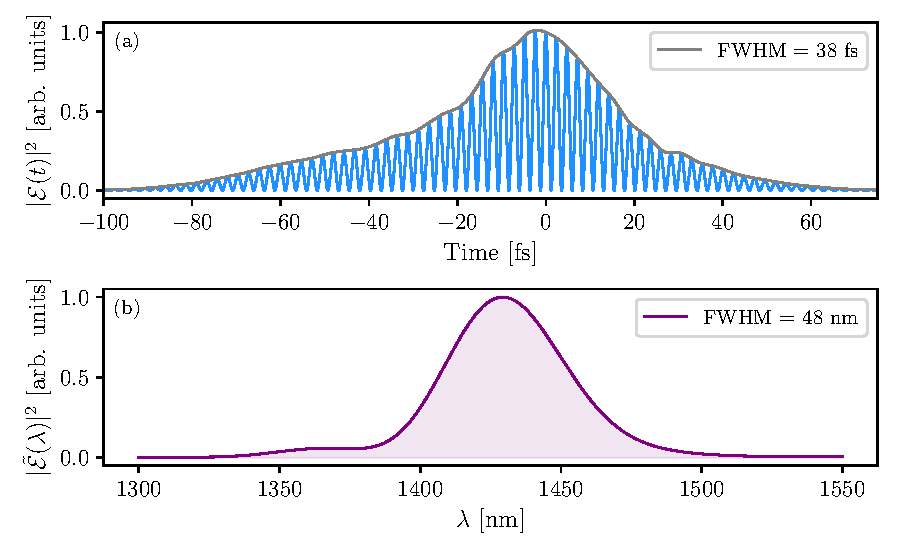
\includegraphics[width=1.0\textwidth]{figures/Beamline/TOPAS_FROG.pdf}
	\caption[Intensity and spectrum of TOPAS output for 1430 nm]{(a) Intensity profile of TOPAS output for a signal wavelength of 1430 nm. (b) Spectrum of TOPAS output for the same wavelength.}
	\label{fig:TOPAS_FROG}
\end{figure}

\section{Beamline Design}
\label{sec:full_beamline}
To begin discussion of the design of the TABLe, it is important to lay out the requirements that needed to be met when designing the apparatus. The primary feature common to all of the experiments that use TABLe is that they will involve XUV pulses that have bandwidth between 26 and 300 eV.  One of the challenges of working with wavelengths in this XUV region is that they require the use of high vacuum systems to perform most experiments.  The fundamental reason for this is due the fact that these wavelengths are ionizing radiation, and they will be quickly absorbed in air.  For example, at 50 eV the attenuation length\footnote{Attenuation length is given by the length that the intensity fall to $1/e$ as the beam propagates through a medium.} is approximately 50 $\mu$m for N$_2$ at 760 Torr \cite{henkeLowenergyXrayInteraction1982}.  Therefore, experiments must be performed in vacuum chambers generally in the high vacuum regime below $10^{-6}$ Torr.  An additional requirement is that these experiments are generally pump/probe experiments where the XUV pulse serves as either the pump or the probe and the other role is fulfilled by an IR pulse.  Thus, an interferometer needs to be designed where an input IR beam is split into two arms, one of which will have XUV generated in it.  A final requirement is that the beamline needs to be able to accommodate different end stations.  This is a critical feature because it greatly expands the capabilities of the apparatus beyond the initial experiments that the TABLe was commissioned for, namely transient absorption experiments.
\begin{figure}
	\centering
	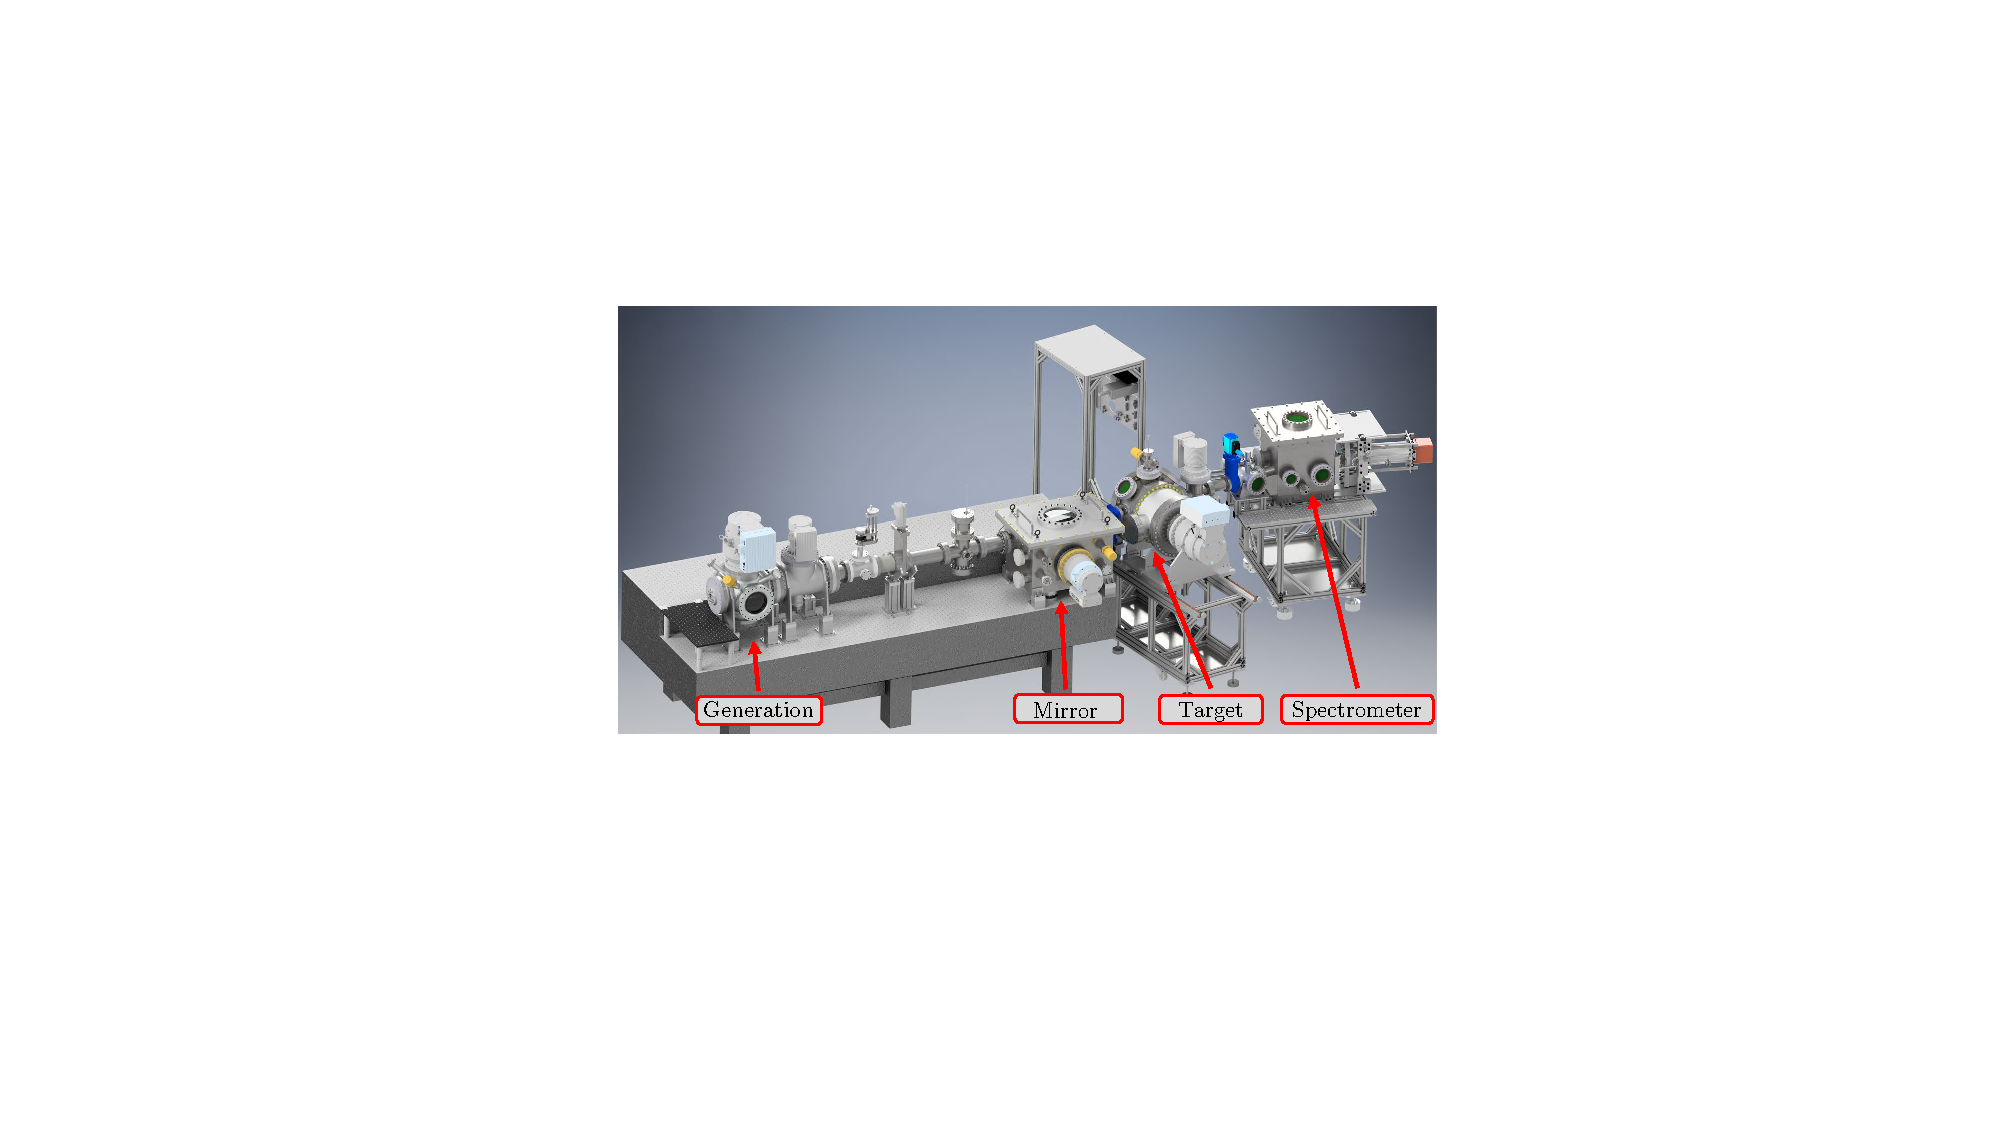
\includegraphics[width=1.0\textwidth]{figures/Beamline/CAD_beamline.pdf}
	\caption[Render of the TABLe]{Render of the Transient Absorption Beamline (TABLe).  The main vacuum chambers are highlighted.}
	\label{fig:CAD_render_TABLe}
\end{figure}
\begin{figure}
	\centering
	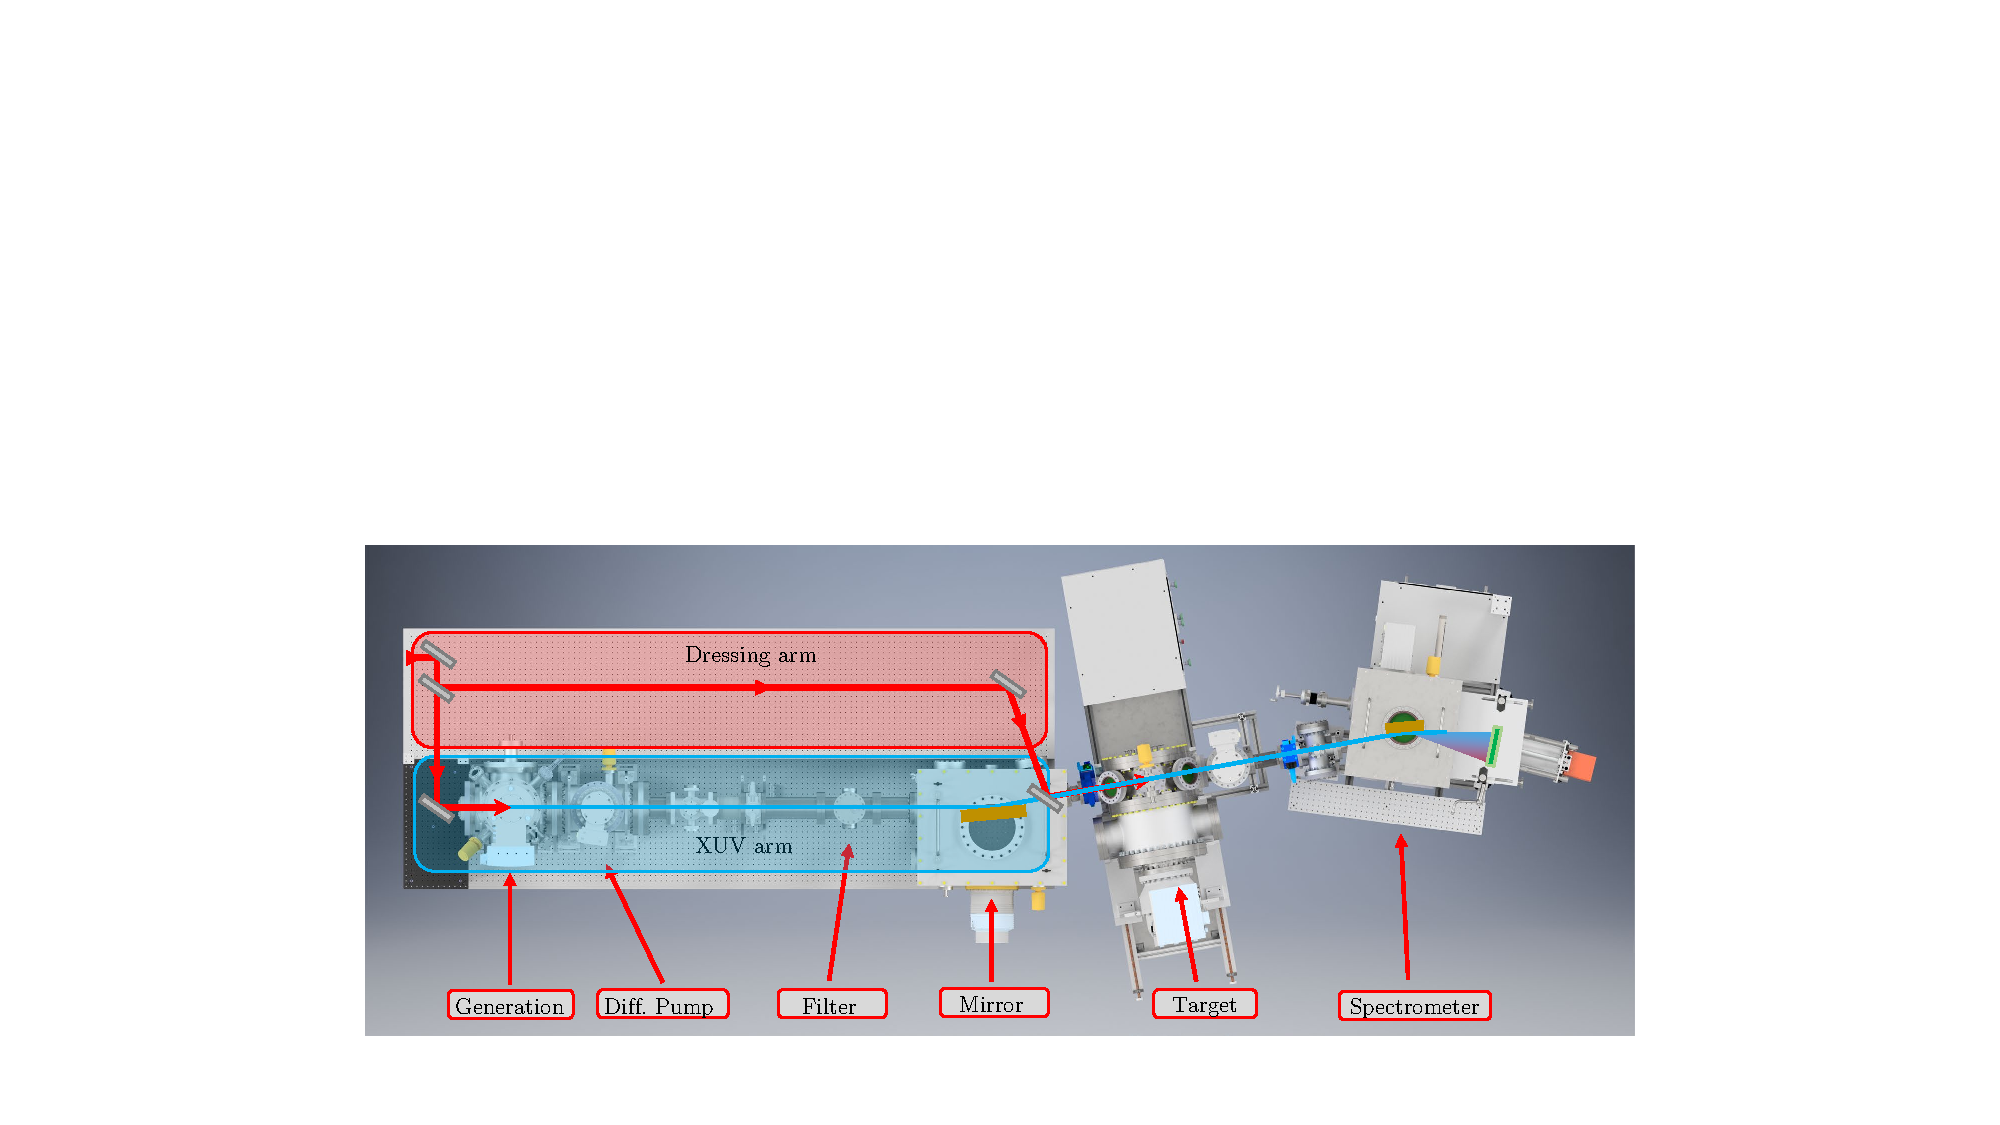
\includegraphics[width=1.0\textwidth]{figures/Beamline/CAD_beamline_top_view.pdf}
	\caption[Top-view render of the TABLe]{Top-view render of the Transient Absorption Beamline (TABLe).  The main vacuum chambers are highlighted, as well as the generation layout of the interferometer with the dressing and XUV arms.  Further details of the exact optical layout can be found in figure \ref{fig:beampath_sketch}.}
	\label{fig:CAD_beamline_top_view}
\end{figure}

The final design of the TABLe is shown in figure \ref{fig:CAD_render_TABLe}, and a top-view of the beamline with a rough schematic of the interferometer is shown in figure \ref{fig:CAD_beamline_top_view}. There are many details about the design and construction that will be left out of this dissertation, however they can be found in great abundance in Greg Smith's dissertation \cite{smithApplicationAttosecondTechniques2020}.  With that being said, the general structure of the vacuum system will be described first, and this consists of several main sections.  The first being the generation chamber which contains the gas source used for HHG.  This chamber is capable of accommodating a variety of gas sources consisting of continuous gas jets, pulsed gas jets, low pressure gas cells, and high pressure gas cells.  Each experiment has different requirements and focal geometries that make any one of these options more advantageous than the others, however the two options that will be used in this dissertation are the high pressure cell and the pulsed gas jet.  The details of the high pressure cell can be found in \cite{smithApplicationAttosecondTechniques2020}.  A picture of the high pressure cell with a laser filament going through it is shown in figure \ref{fig:HPGC_filament}.  The distinguishing feature of the high pressure cell is its ability to achieve interaction pressures up to several bar through the use of a pair concentric tubes that the allow for differential pumping.  The primary disadvantages are the difficulty in initial alignment and the restrictive set of four holes that the laser must propagate through.  This make the high pressure cell untenable for some experiments, such as those described in Chapters \ref{chap:two_source}, \ref{chap:refractive_index}, and \ref{chap:CATS}.  An alternative to the gas cell is the pulsed gas jet.  This work by using a piezoelectric actuator to block gas from exiting a gas nozzle and only let out a pulse of gas at a fixed frequency and duty cycle.  This operation mode means that the average background pressure within the vacuum is lower than just a simple continuous gas jet operation, but the interaction pressure can be the same.  A picture of the pulsed jet in operation is shown in figure \ref{fig:piezo_jet}.
\label{sec:gas_source}
\begin{figure}
	\centering
	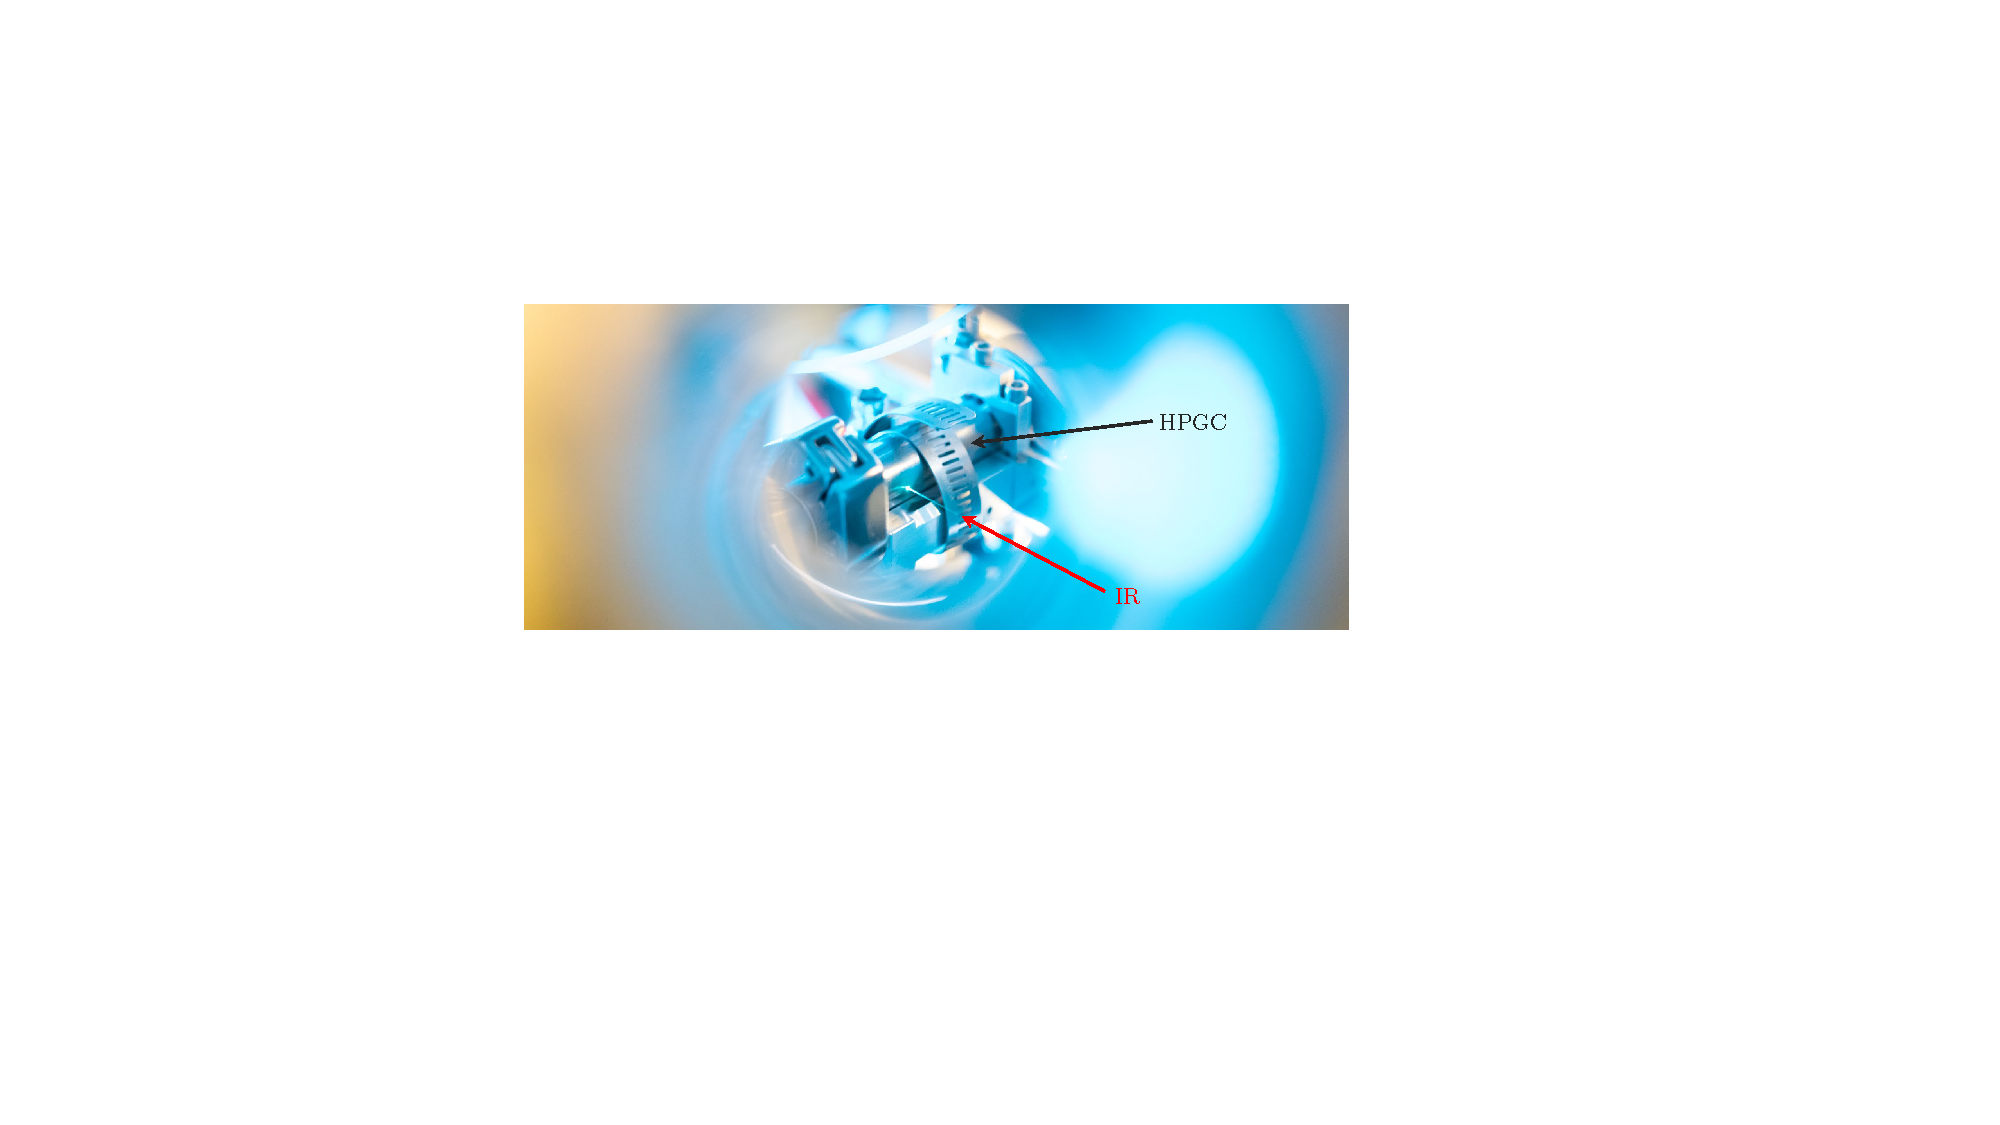
\includegraphics[width=0.8\textwidth]{figures/Beamline/HPGC.pdf}
	\caption[Image of laser passing through HPGC]{Camera image of IR laser filament pass through the high-pressure gas cell (HPGC) during alignment at atmospheric conditions.}
	\label{fig:HPGC_filament}
\end{figure}


Following a differential pumping section, there is a metallic spectral filter assembly.  This is used to place a metallic filter that is generally on the order of a few hundred nanometers into the beam path of the XUV.  The primary reason for this is to block the co-propagating IR field that is used to generate the XUV pulse.  However, it can also be used to shape the spectrum and phase of the XUV pulse to suit the experimental requirements \cite{chiniGenerationCharacterizationApplications2014}.  The transmission function of three of the most common filter materials is shown in figure \ref{fig:filters}.  As can be clearly seen, different materials have significantly different bandpass windows, and this is due to each elements atomic structure and the transition energy of the core level.  For example, Al is the filter that is most commonly used for these experiments, and it transmits reasonably well below the $L$-edge which occurs at 72.3 eV, however it strongly absorbs above this energy.
\begin{figure}
	\centering
	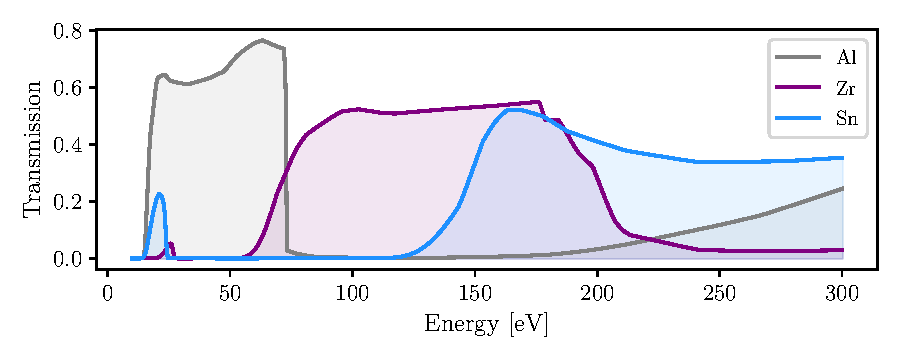
\includegraphics[width=0.9\textwidth]{figures/Beamline/filters.pdf}
	\caption[Transmission of several metallic filters]{Transmission as a function of photon energy for several metallic filters.  All filters are 200 nm thick.}
	\label{fig:filters}
\end{figure}

The next main section of the TABLe that must be described is the mirror chamber.  This section houses the primary XUV focusing optic, the ellipsoidal mirror.  Again, much greater detail can be found in \cite{smithApplicationAttosecondTechniques2020}, however the key features of this special optic will be discussed here.  A significant challenge with working in this energy range is the lack of efficient and broadband optics.  This is due to the strong absorption by most materials when they are used near normal incidence.  There are two main methods that have been employed to overcome this: grazing incidence optics or multilayer optics \cite{attwoodSoftXraysExtreme2000}.  Each have their advantages and disadvantages, but generally grazing incidence optics operate over a much larger bandwidth.  This was a key design criteria for the TABLe, so a grazing incidence optic was selected to refocus the XUV beam.  There are several designs that can be used to refocus a beam using a grazing incidence optics, and the one that was selected was the ellipsoidal mirror.  The significant advantage of this type of optic is that is can re-image a point source aberration free with demagnification.  The geometric optics principle behind this is highlighted in figure \ref{fig:ellipsoid}.  The ellipsoid that was chosen for the TABLe has an entrance arm of 2250 mm and an exit arm of 750 mm, thus giving a demagnification of 3.  This allows for smaller XUV spot sizes to be used.
\begin{figure}
	\centering
	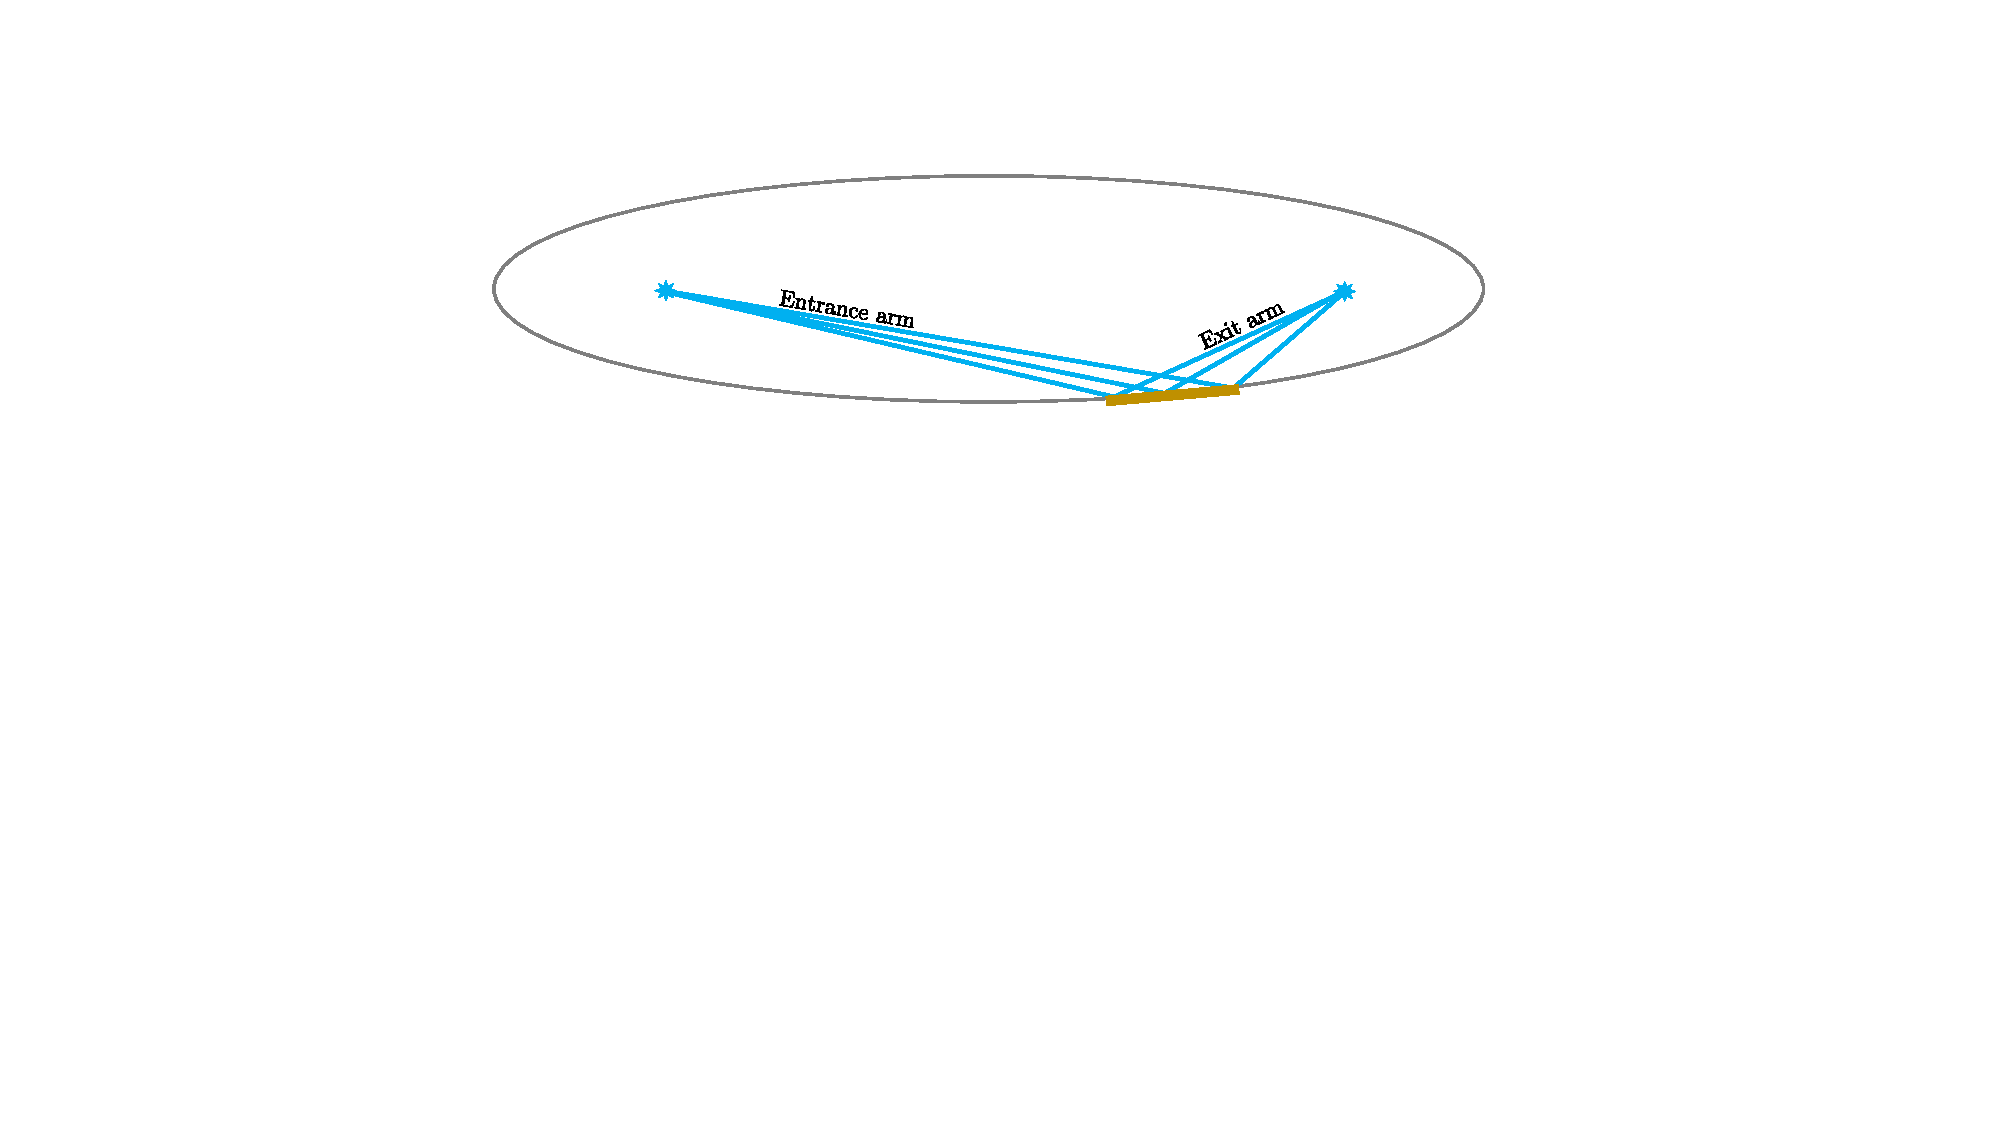
\includegraphics[width=0.8\textwidth]{figures/Beamline/ellipsoid.pdf}
	\caption[Schematic of ellipsoidal mirror]{Schematic of ellipsoidal mirror.  From geometric optics, the ellipsoidal mirror will focus all rays from a point source at one foci of the ellipse to the other foci.  The ratio of the exit arm to the entrance arm is the magnification provided by the mirror.}
	\label{fig:ellipsoid}
\end{figure}

The next major section of the TABLe is the target chamber.  As the name implies, this is where the sample of interest for an experiment is placed.  This chamber is capable of housing both condensed matter samples in the form of free standing membranes and a gas cell to perform gas phase measurements.  The two configurations that the target chamber can operate in is shown in figure \ref{fig:gas_solid_sample_holder}. 
\begin{figure}
	\centering
	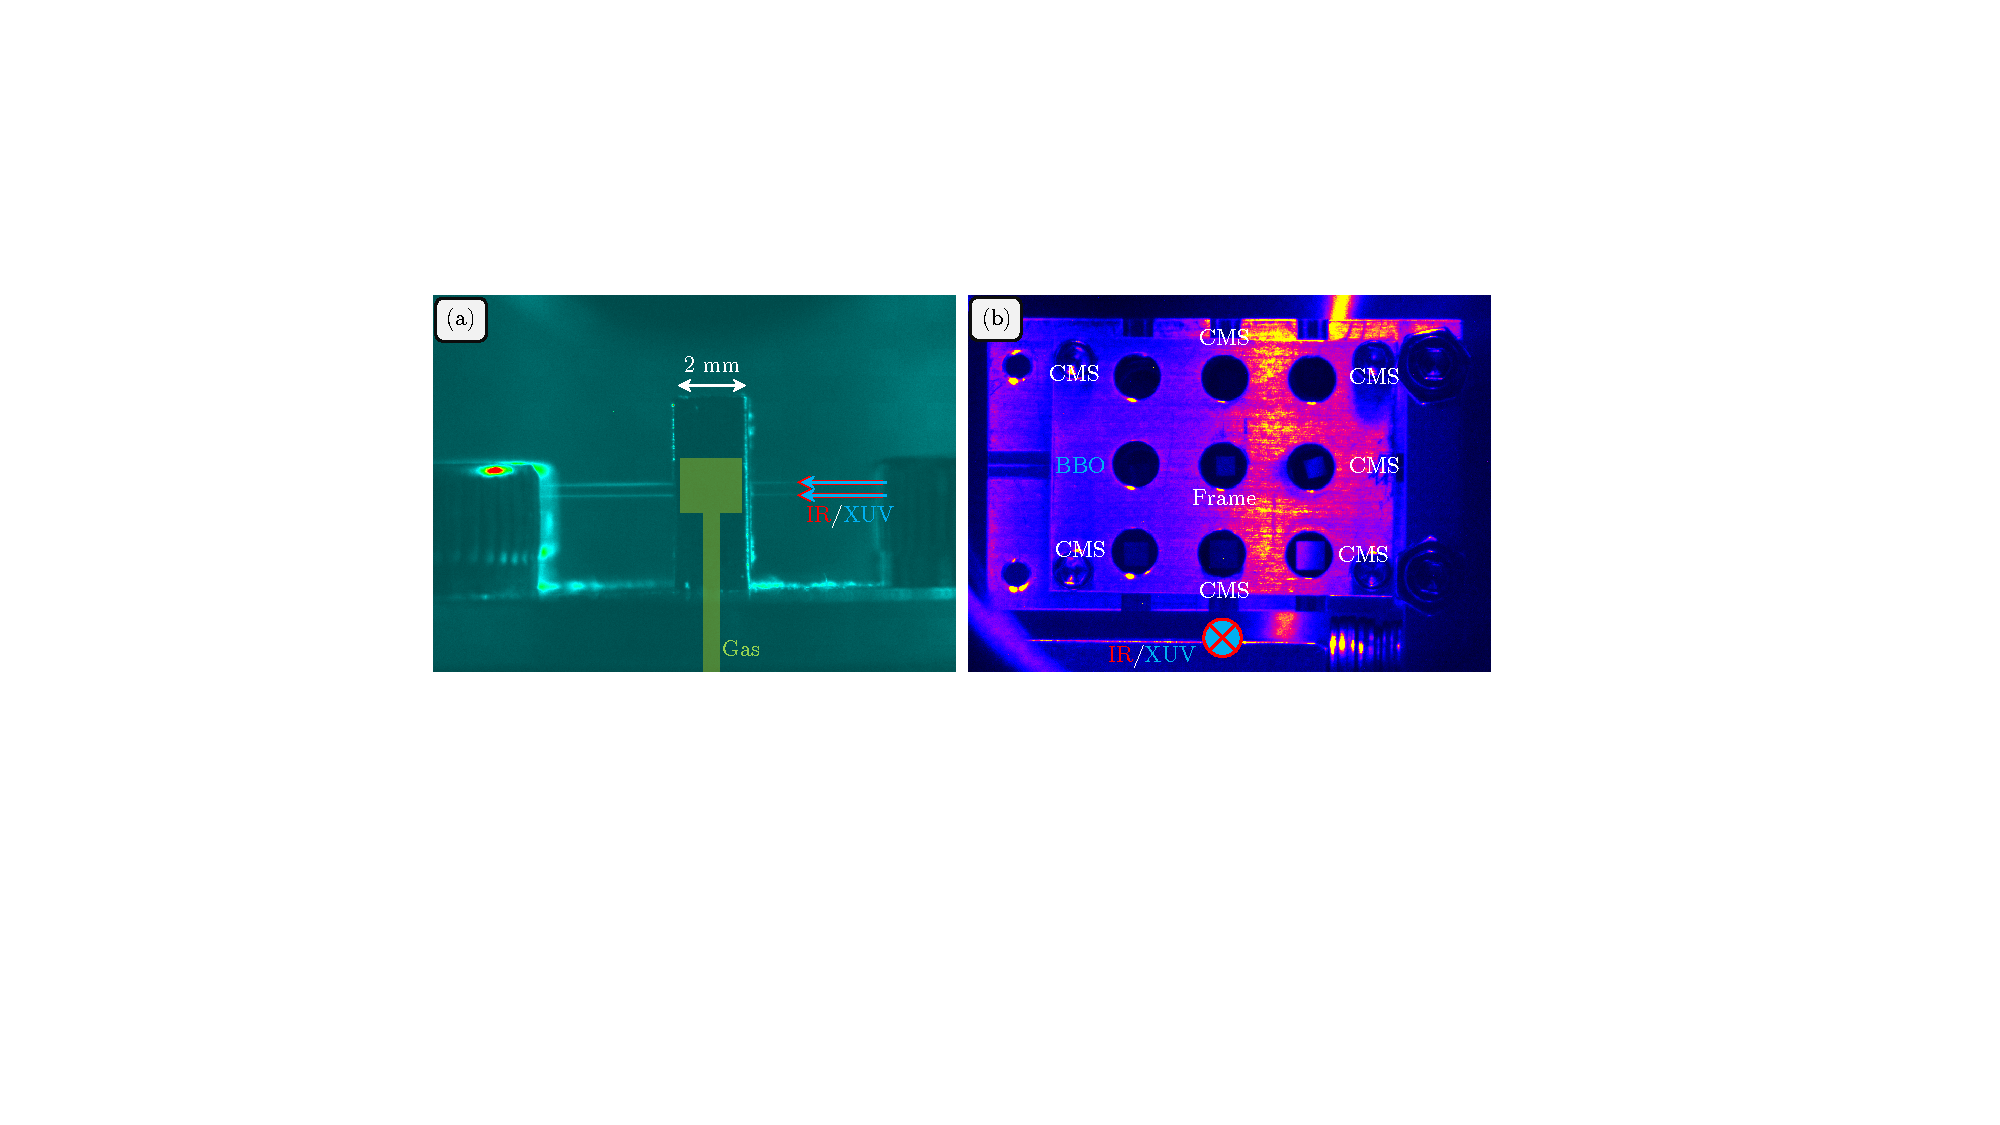
\includegraphics[width=0.9\textwidth]{figures/Beamline/gas_solid_sample_holder.pdf}
	\caption[Camera image of target gas cell and condensed matter sample holder]{(a) Camera image of the gas cell used for gas phase experiments. Two sources IR sources are generating a filament. Image was taken while chamber was vented and at ambient pressure. (b) Camera image of the condensed matter sample holder.  This was taken \textit{in-situ} while under vacuum.  The sample holder is generally configured to carry six condensed matter samples (CMS), one BBO to find temporal overlap, and one empty frame to perform knife-edge measurements.  The IR/XUV beams propagate into the page for this image.}
	\label{fig:gas_solid_sample_holder}
\end{figure}

Finally, the last major component of the TABLe that needs to be discussed is the photon spectrometer.  This home-built spectrometer was commissioned to perform the experiments described in this dissertation as well as those described in \cite{smithApplicationAttosecondTechniques2020}.  The design criteria that this spectrometer had to meet was that it had to be a high resolution spectrometer covering a spectral range from 20 eV all the way through the Carbon $K$-edge at 284 eV.  This was chosen because of eventual plans to perform transient absorption experiments in the water-window at the Carbon $K$-edge, while still maintaining the ability to do more reasonable experiments at lower photon energies in the 20 - 100 eV range.

This is a massive bandwidth to cover with high resolution, so the decision was made to use two different grating to cover this full spectral range.  The gratings that were selected are concave spherical variable line spaced (VLS) gratings produced by Hitachi.  A schematic of the grating is shown in figure \ref{fig:Hitachi_gratings}, and the relevant design parameters for the gratings are given in table \ref{tab:vls_gratings}.  The advantage of a VLS grating design is that they combine the focusing and dispersive optics that are generally needed into a single optic that performs both functions.  Furthermore, these gratings are designed to focus a specific spectral bandwidth onto a plane (as opposed to the typical Rowland circle \cite{rowlandConcaveGratingsOptical1883, pedrottiIntroductionOptics2007}), and this means that a large bandwidth can be in focus on a detector at a single position.  This can be seen in figure \ref{fig:VLS_flat_field} where the focal plane for a range of wavelengths is shown for both grating. This is calculated using the relationship between the entrance $r$ and exit arm $r'$ at an incidence angle $\theta_i$ is given by
\begin{equation}
	r' = \frac{r R (\cos\theta_r)^2}{m\lambda\sigma_0 b_2 + r(\cos\theta_i + \cos\theta_r) - R(\cos\theta_i)^2}
\end{equation}
where $R$ is the radius of curvature, $m$ is the diffraction order, $\theta_r$ is given by
\begin{equation}
	\sin\theta_i + \sin\theta_r = m\sigma\lambda,
\end{equation}
and $b_2$, $\sigma$, $\sigma_0$ are given by 
\begin{equation}
	\sigma(w) = \frac{\sigma_0}{1 + \frac{2b_2}{R}w + \frac{3b_3}{R^2}w^2 + \frac{4b_4}{R^3}w^3 + ...}
\end{equation}
which is the groove density along the face of the grating $w$ \cite{polettoGrazingincidenceFlatfieldSpectrometer2001, haradaMechanicallyRuledAberrationcorrected1980, haradaOptimumDesignGrazingincidence1999}.
\begin{figure}
	\centering
	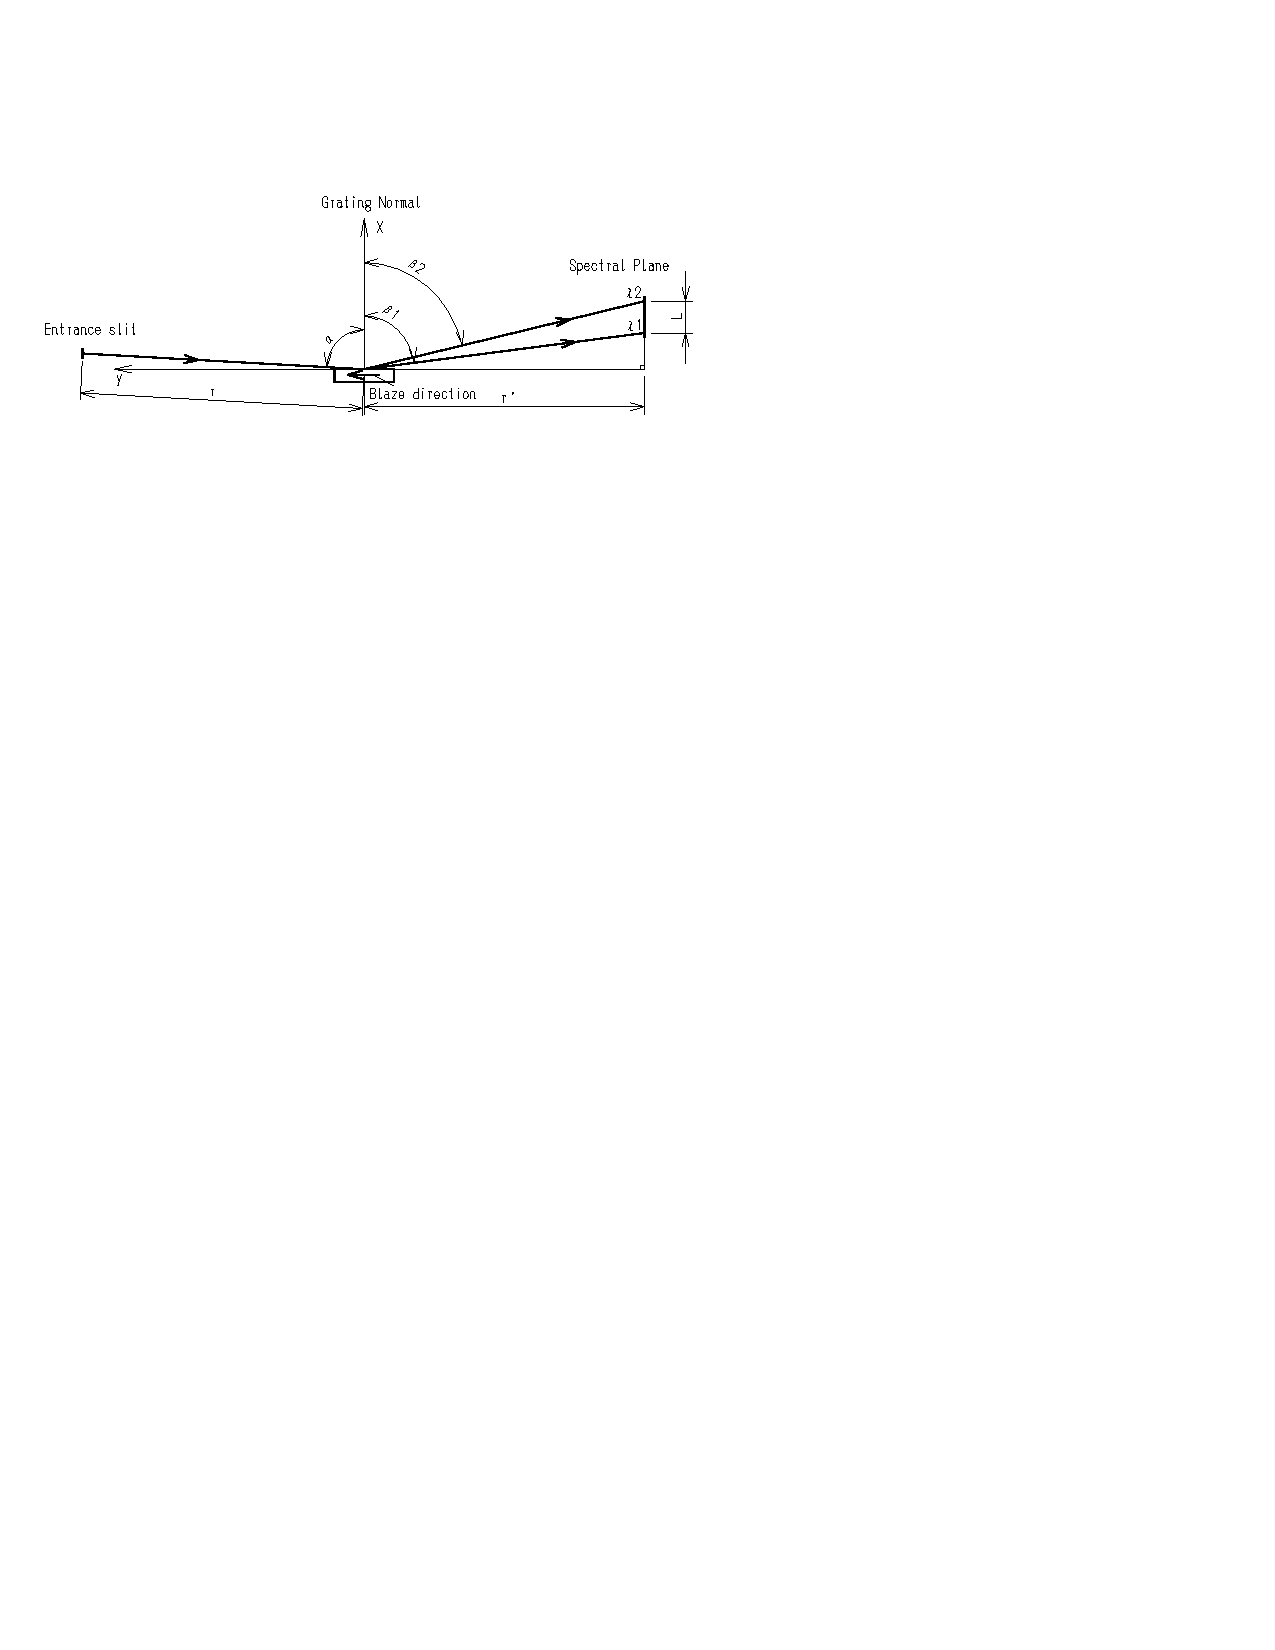
\includegraphics[width=0.8\textwidth]{figures/Beamline/Hitachi.pdf}
	\caption[Schematic of VLS grating]{Schematic of VLS grating with the design parameters $r$ (distance from slit to center of grating), $r'$ (distance from center of grating to image plane), and $L$ (the length of the spectral range that is in focus between $\lambda_1$ and $\lambda_2$).}
	\label{fig:Hitachi_gratings}
\end{figure}
\begin{table}[]
	\centering
	\begin{tabular}{|c|c|c|c|c|c|c|c|}
		\hline\hline
		lines/mm & \begin{tabular}[c]{@{}c@{}}Blaze \\ $\lambda$ {[}nm{]}\end{tabular} & $\alpha$ & r {[}mm{]} & r' {[}mm{]} & $\beta_1$ & $\beta_2$ & $\lambda_1$-$\lambda_2$ \\ \hline
		1200     & 10                                                                  & 87       & 237        & 235.3       & -83.04    & -77.07    & 5-20                    \\ \hline
		2400     & 1.5                                                                 & 88.7     & 237        & 235.3       & -85.81    & -81.01    & 1-5                     \\ \hline\hline
	\end{tabular}
	\caption[Parameters of Hitachi VLS gratings]{Parameters of Hitachi VLS gratings.}
	\label{tab:vls_gratings}
\end{table}

\begin{figure}
	\centering
	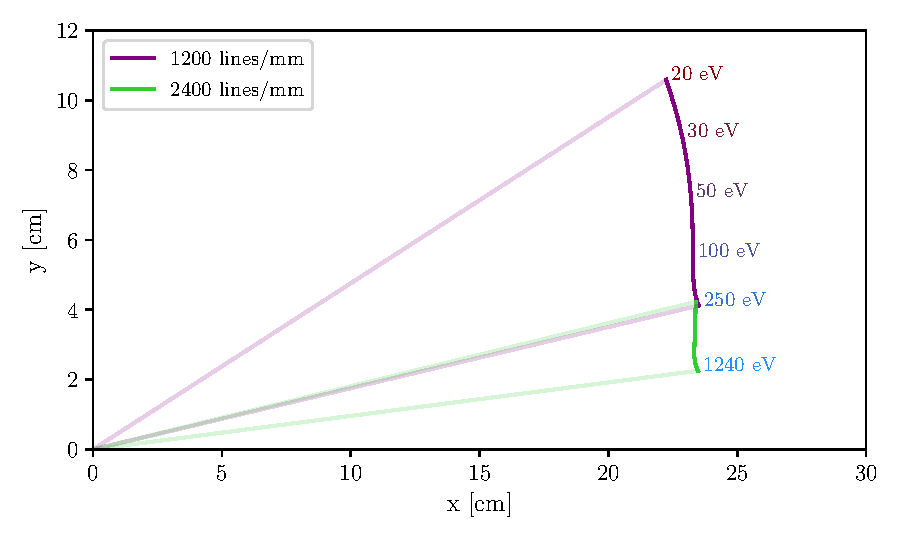
\includegraphics[width=0.9\textwidth]{figures/Beamline/VLS_flat_field.pdf}
	\caption[Flat field of VLS gratings]{Flat fields of the two VLS grating that comprise the photon spectrometer.  The $x$ axis is parallel to the face of the grating, and the $y$ axis is perpendicular to the grating face.  The center of the grating is located at (0,0).  Incidence angle and entrance arm are those provided in table \ref{tab:vls_gratings}.}
	\label{fig:VLS_flat_field}
\end{figure}




Another design criteria for this spectrometer was that it had to be able to be used on a variety of different systems.  The modular design of the TABLe meant that this spectrometer could be removed from the TABLe and brought to a different light source.  This entails that the entrance arm could be different from the one specified by the manufacturer depending upon the system that is installed in.  To account for this change in entrance arm, the angle of the grating can be changed from the specified one to recover the flat field condition.  This can be seen for both gratings in figure \ref{fig:variable_flat_field}.  Of course, one issue with this approach is that even though the flat field can be recovered, the grating efficiency changes as a function of angle.  This can be done numerically, and there are many packages available to perform these calculations. The grating efficiency for the 1200 lines/mm grating was calculated in \cite{hageDevelopmentXUVSpectrometer}, and the results are shown in figure \ref{fig:grating_efficiency}.  As can be clearly seen, the efficiency changes non-trivially as a function of grazing angle for a given wavelength.  Thus, depending upon the position of the detector and the photon energy of interest, there is a different incident angle that can be selected to optimize the grating efficiency.
\begin{figure}
	\centering
	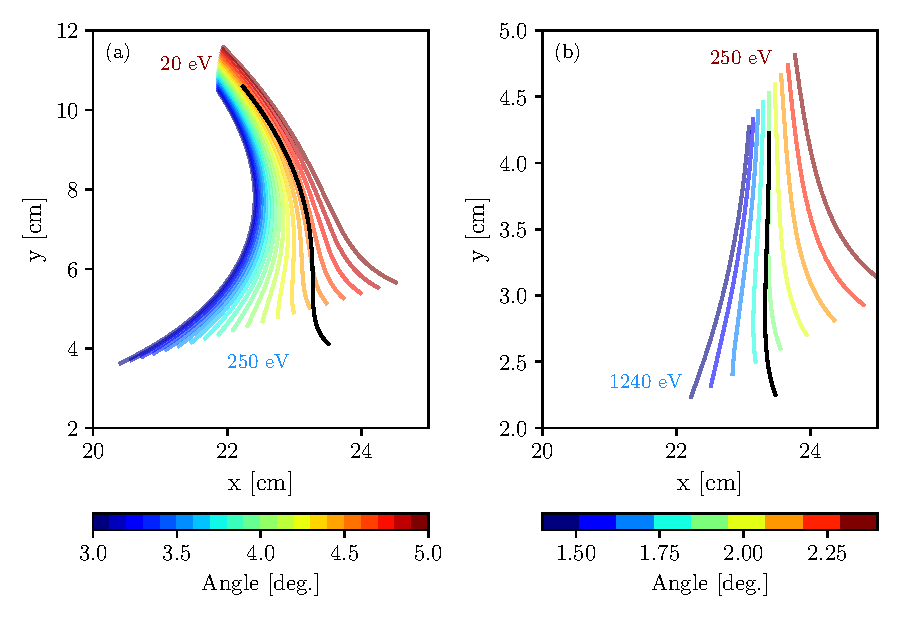
\includegraphics[width=0.9\textwidth]{figures/Beamline/variable_flat_field.pdf}
	\caption[Flat field of both VLS gratings as a function of input angle]{Flat field calculated as a function of incident angle for an entrance arm of 1.5 m.  The flat field for the manufacturers specified entrance arm of 0.237 m is shown in black. (a) is for the 1200 lines/mm VLS grating and (b) is for the 2400 lines/mm VLS grating. The $x$ axis is parallel to the incident light, and teh $y$ axis is perpendicular to the incident light.}
	\label{fig:variable_flat_field}
\end{figure}

\begin{figure}
	\centering
	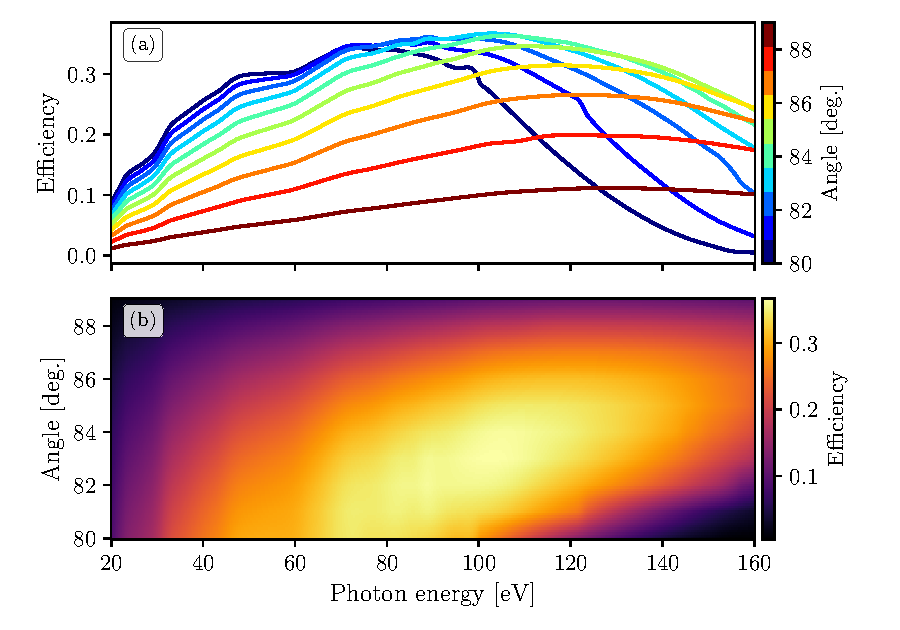
\includegraphics[width=0.9\textwidth]{figures/Beamline/grating_efficiency.pdf}
	\caption[VLS grating efficiency as a function of incident angle and photon energy]{Calculated VLS grating efficiency as a function of grazing angle and photon energy.  Shown as a series of line outs in (a) and as an interpolated heat map in (b).  Data is obtained from \cite{hageDevelopmentXUVSpectrometer}.}
	\label{fig:grating_efficiency}
\end{figure}

\begin{figure}
	\centering
	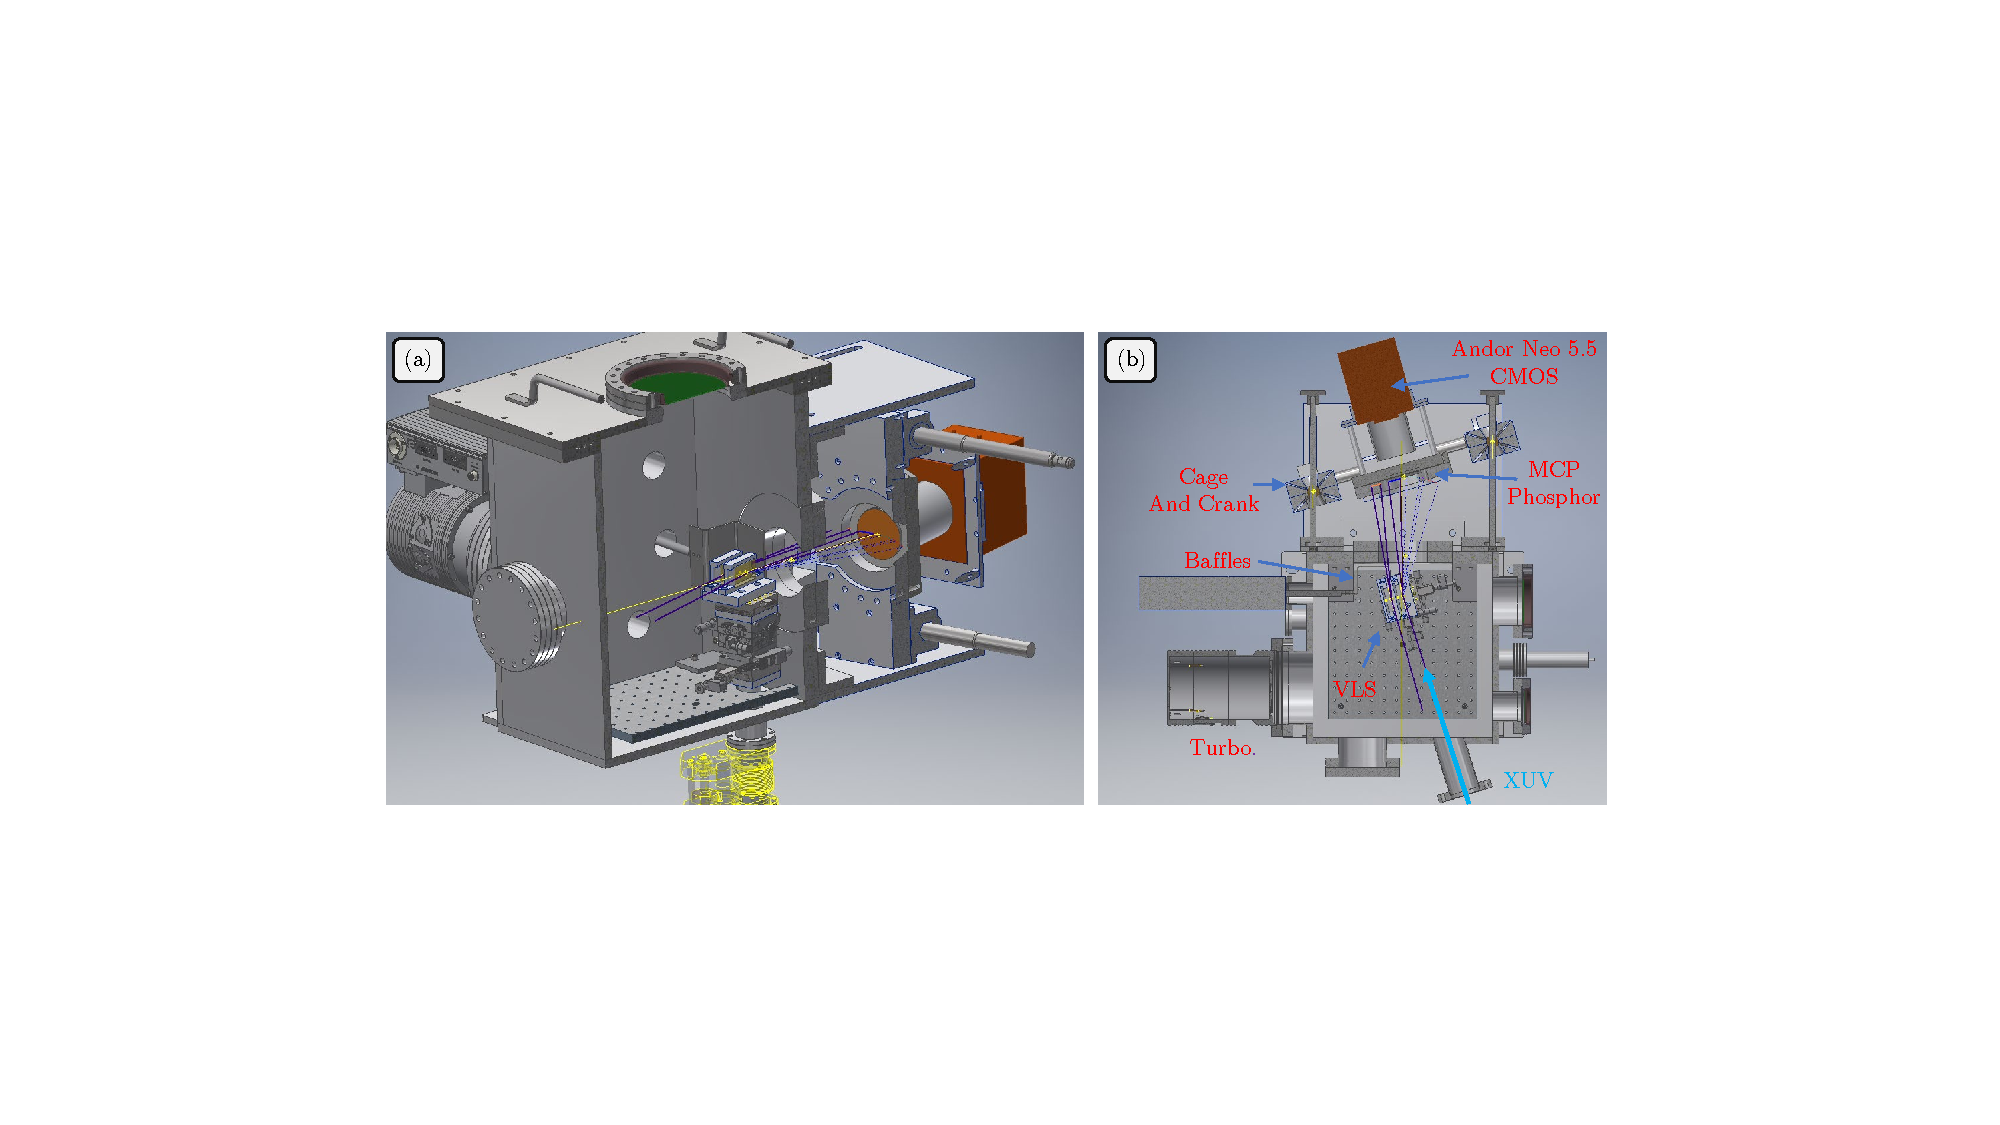
\includegraphics[width=0.9\textwidth]{figures/Beamline/CAD_spectrometer.pdf}
	\caption[CAD render of the TABLe spectrometer]{Render of the spectrometer showing a side-view (a) and a top-view (b).}
	\label{fig:CAD_spectrometer}
\end{figure}

Now it is time to move on to the actual design of the spectrometer, and a render of the spectrometer is shown in figure \ref{fig:CAD_spectrometer}. This design has the capability to switch between the two diffraction gratings while under vacuum through the use of 6-axis motorized control.  The detector consists of a 75 mm imaging quality micro-channel plate (MCP) and phosphor that is mounted on an 8" ConFlat flange.  The output of the phosphor is re-imaged onto an Andor Neo 5.5 CMOS camera using a 50 mm focal length lens.  The MCP was selected over a direct detection XUV CCD camera because of the much larger detector area that can be achieved using an MCP. To position this detector along the focal plane for each grating, a custom manipulator was developed, and this manipulator is referred to as the cage and crank.  It consists of three screws that allow for the tilt and translation of the detector while the chamber is under vacuum.  This allows for optimization of the resolution in different parts of the harmonic spectrum based upon the experimental needs.  An example of the phosphor output is shown in figure \ref{fig:spectrometer_output} (a) for a case where the phosphor emission was bright enough that it could be easily seen by eye, and an example of a typical image taken by the Andor camera is shown in figure \ref{fig:spectrometer_output} (b).  These images constitute the basis of all of the experiments that are described within this dissertation, and there are a couple of key features that are important to highlight.  As a consequence of selecting VLS gratings, the resulting spectrum that is measured is only focused along the spectral dimension, as shown in figure \ref{fig:spectrometer_output} (b), and the other dimension, generally referred to as the spatial dimension,  is unfocused and allows for the measurement of the spatial profile of the XUV beam as a function of energy.  This allows for unique measurements to be performed that involve the spatial interference of two XUV beams, and this capability is what enables the experiments in Chapters \ref{chap:two_source}, \ref{chap:refractive_index}, and  \ref{chap:CATS}.


\begin{figure}
	\centering
	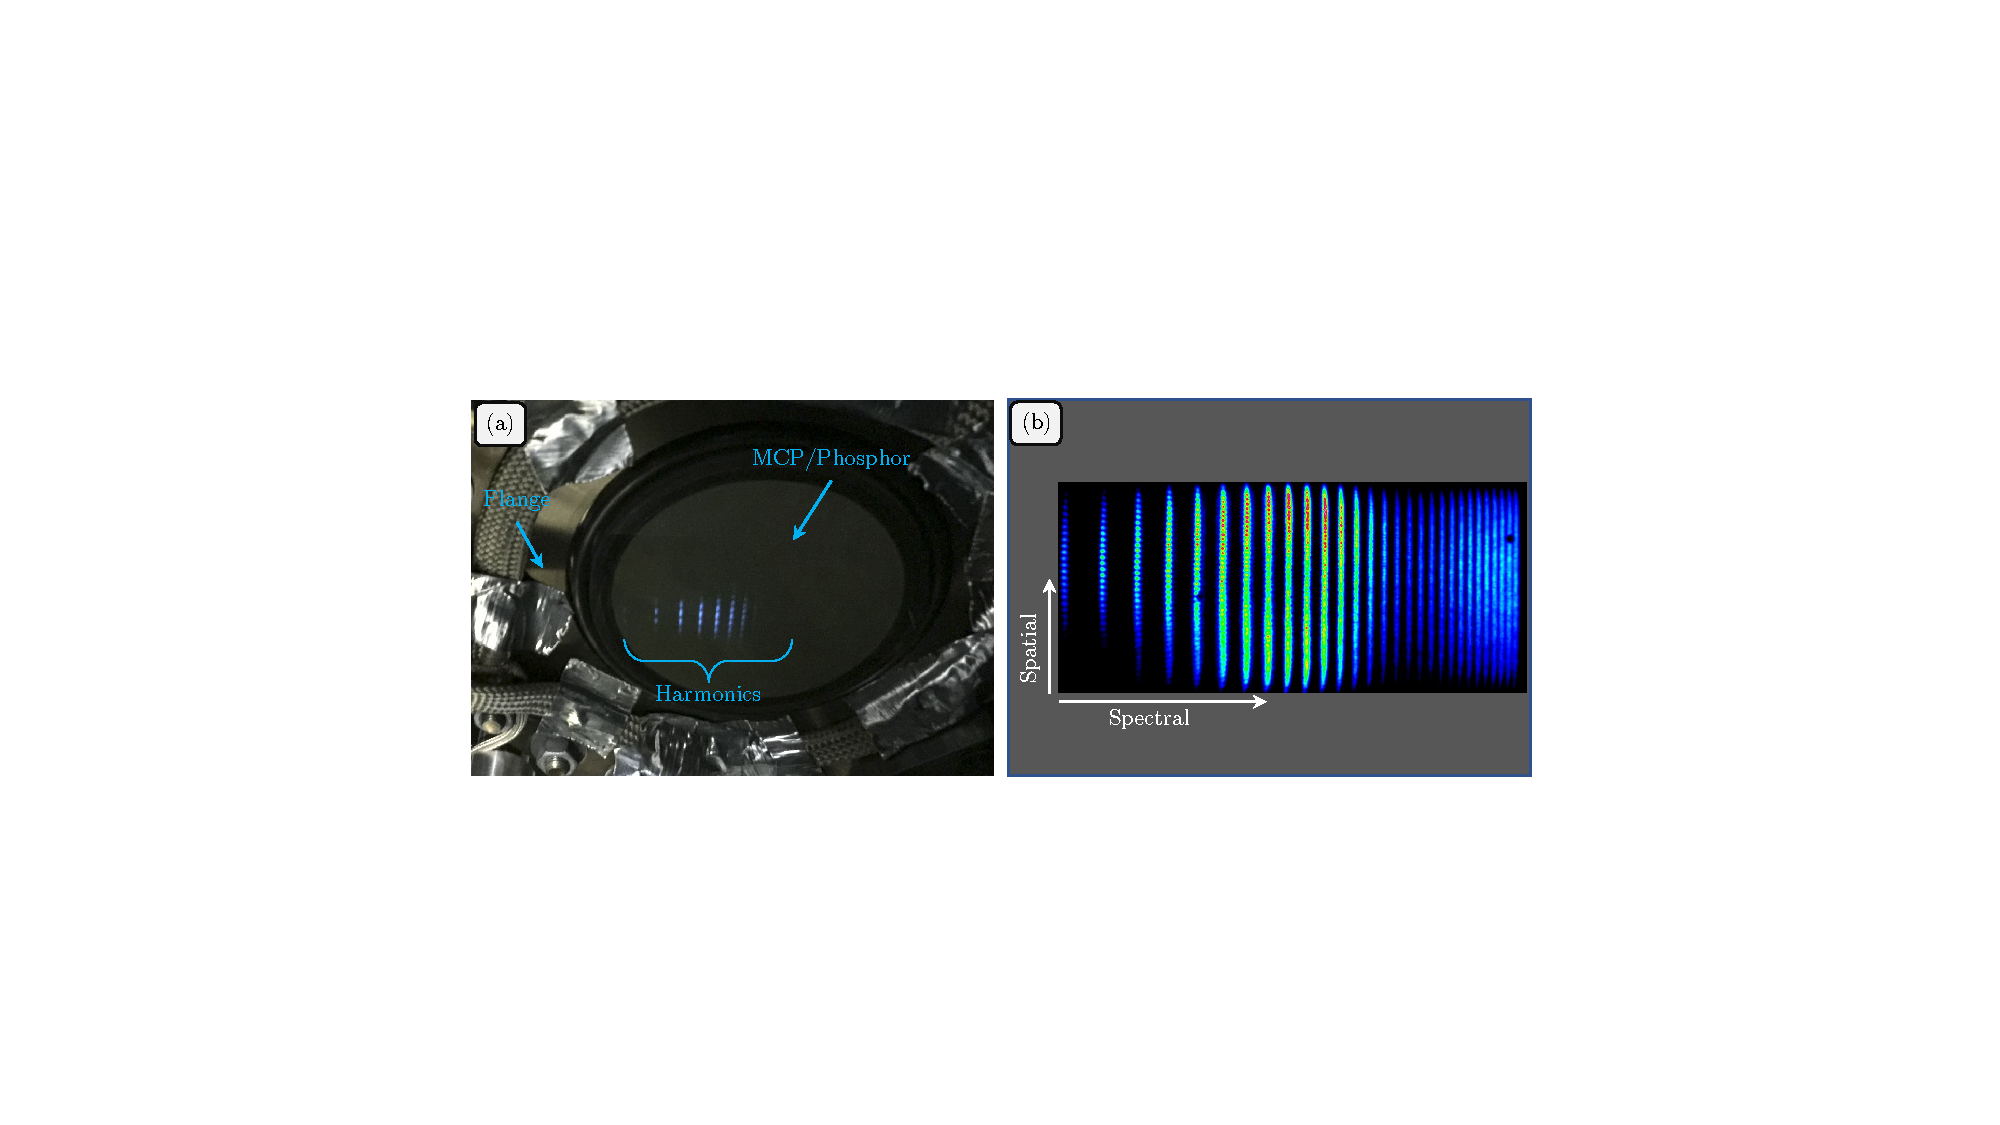
\includegraphics[width=0.9\textwidth]{figures/Beamline/spectrometer_output.pdf}
	\caption[Image of phosphor output of high harmonics generated from two sources and sample data image]{(a) Camera image of the output of the phosphor screen.  Harmonics are visible by eye.  (b) Sample data image collected from the Andor high-resolution camera.  Spatial and spectral structure of the XUV APT can be seen.}
	\label{fig:spectrometer_output}
\end{figure}

Finally, the last important consideration of the spectrometer is its maximum achievable resolution.  This can be done by calculating the energy difference between two points that are separated by the effective pixel size along the flat field curve.  This calculation is shown in figure \ref{fig:grating_resolution} for both gratings.  In the energy range of 20-80 eV, the resolution $\Delta E/E$ of the 1200 lines/mm grating ranges from $1\times10^{-3}$ to $2\times10^{-3}$.  This resolution is fundamentally limited by the effective pixel size, and it can be improved by a factor of 4 if a different re-imaging lens is used for the Andor camera. Further resolution improvements can be made by using a direct detection XUV CCD camera with smaller pixel sizes.
\begin{figure}
	\centering
	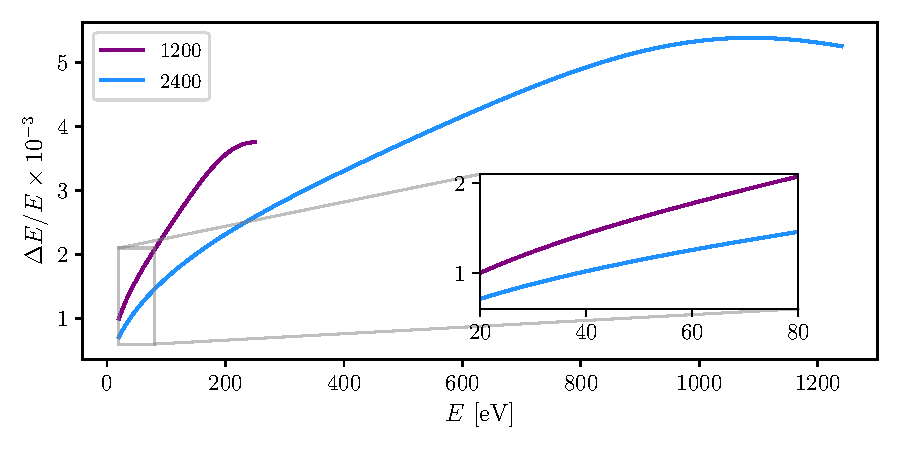
\includegraphics[width=0.9\textwidth]{figures/Beamline/grating_resolution.pdf}
	\caption[Maximum achievable resolution for VLS gratings]{Maximum achievable resolution for the 1200 and 2400 lines/mm VLS gratings. Calculated using an effective pixel size of 48 $\mu$m.  Inset shows the spectral region that will be important for the experiments described herein.}
	\label{fig:grating_resolution}
\end{figure}



\section{Optical layout}
\label{sec:optical_layout}

Now that the design of the TABLe has been covered, attention can now be turned to the optical layout of the TABLe.  As stated previously, the TABLe is designed around performing pump/probe experiments using both XUV and IR pulses.  This is done by building a Mach-Zehnder interferometer where one arm is IR and the other arm is used to generate the XUV APT.  The optical layout that was implemented is shown in figure \ref{fig:beampath_sketch}.  This setup was designed to use the signal wavelengths from the TOPAS over the 1250-1550 nm range, and it can accommodate a wavelength change within this range with minimal adjustment of the interferometer.  In the following sections several major components that determine the interferometer performance will be highlighted, and the two different XUV generation schemes that are used will be described in Chapter \ref{chap:two_source} and \ref{chap:ATS}.

\begin{sidewaysfigure}
	\centering
	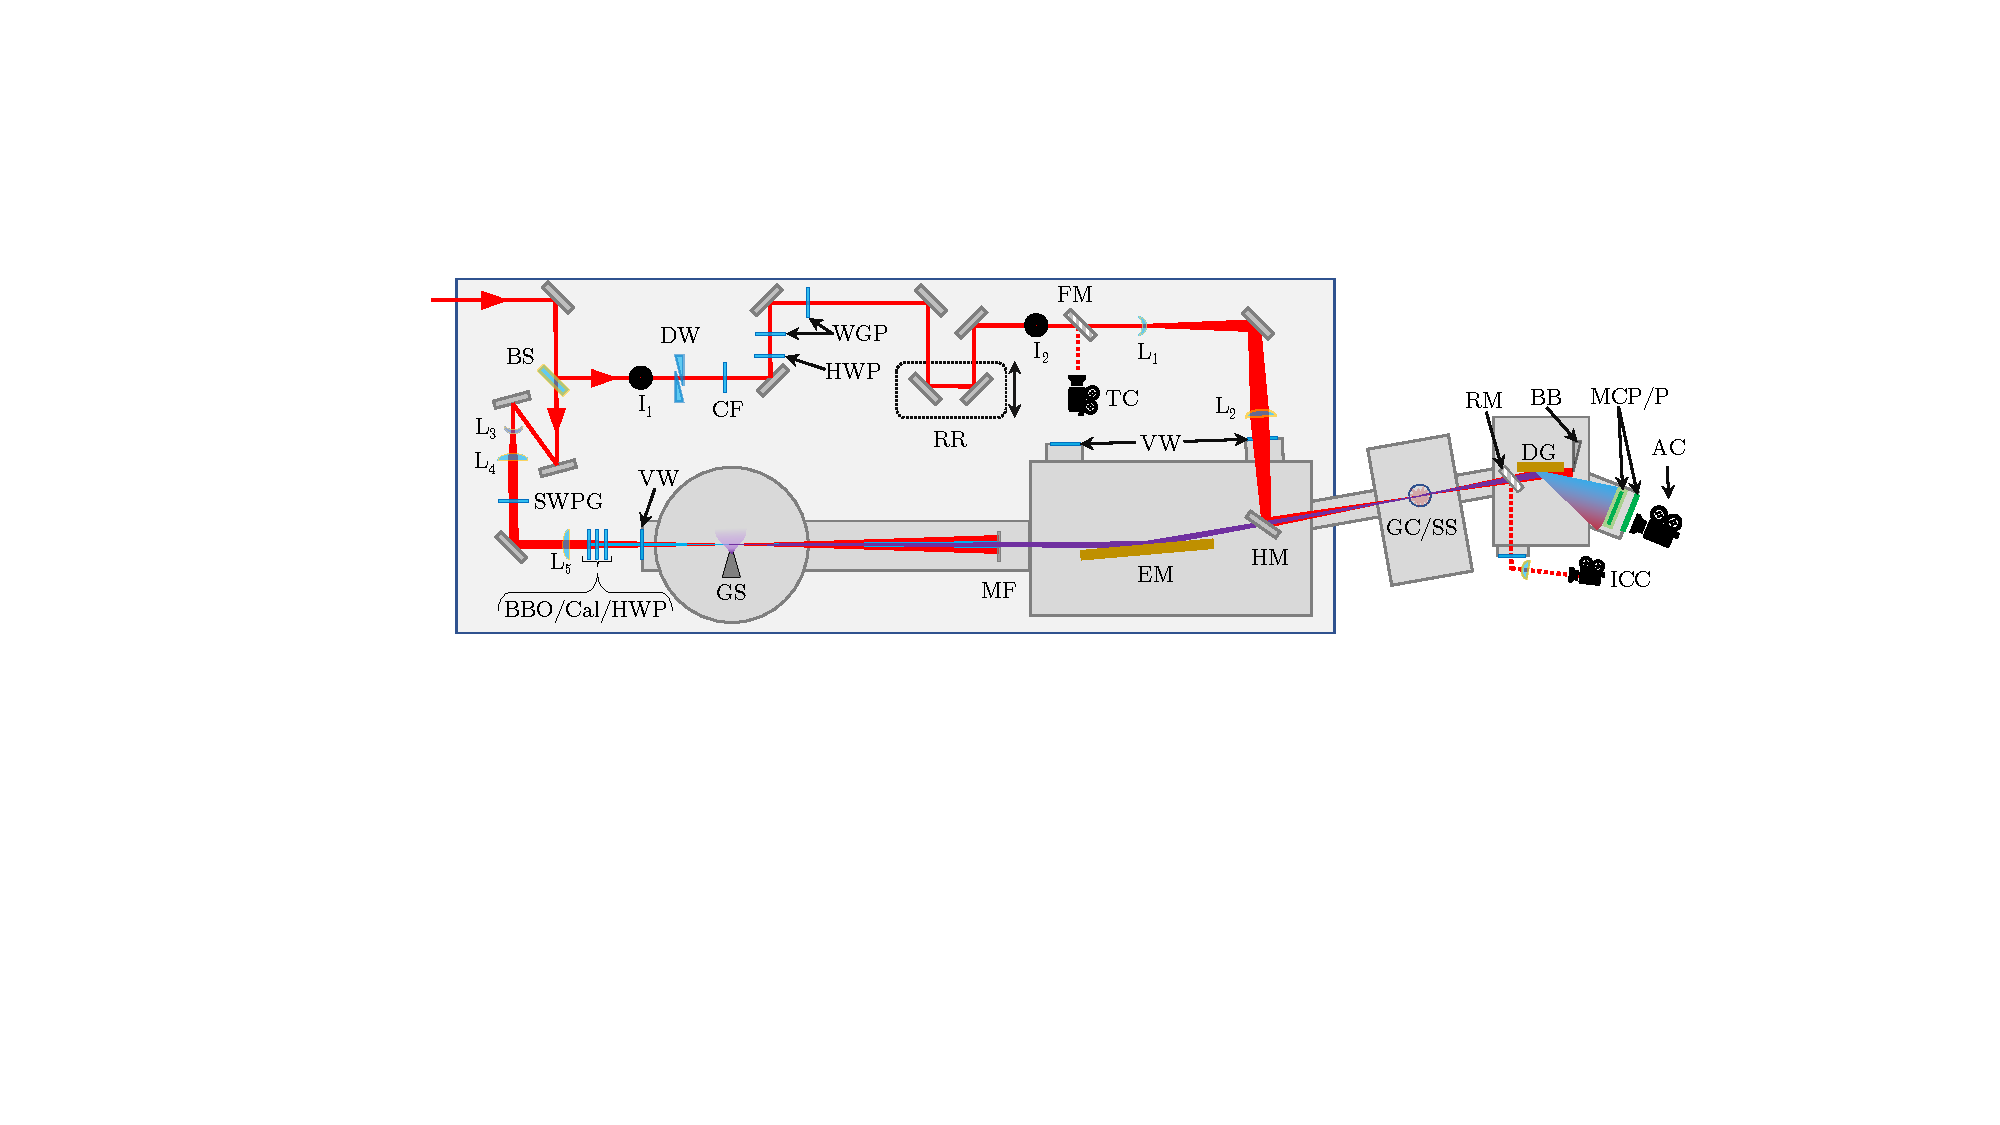
\includegraphics[width=1.0\textwidth]{figures/Beamline/beampath_sketch_3.pdf}
	\caption[Schematic of TABLe optical layout.]{Schematic of the beam path for the TABLe interferometer. The input laser is shown in red, its second harmonic in  blue, and the generated XUV in purple.  \textbf{BS}: Beamsplitter (Thorlabs BSF20-C), \textbf{I$_1$} and \textbf{I$_2$}: Irises used for alignment into interferometer. \textbf{DW}: Delay wedges for fine delay control, see section \ref{sec:delay_wedges}. \textbf{CF}: Color filter to remove parasitic colors from TOPAS (Thorlabs FELH1000). \textbf{HWP}: Half-wave plate. \textbf{WGP}: Wire grid polarizer. \textbf{RR}: Retro reflector for coarse delay adjustment.  \textbf{FM}: Flip mirror. \textbf{TC}: Thermal camera used for alignment.  \textbf{L$_1$}: $f=-300$ mm lens (Thorlabs LF1015-C). \textbf{L$_2$}: $f=500$ mm lens (Thorlabs LA1380-C). \textbf{VW}: Vacuum window, 3 mm CaF$_2$, \textbf{HM}: Hole mirror with 10 mm hole.  \textbf{L$_3$}: $f=-400$ mm lens.  \textbf{L$_4$}: $f=500$ mm lens. \textbf{SWPG}: Square-wave phase grating. \textbf{L$_5$}: $f=400$ mm lens.  \textbf{BBO}: Second-harmonic generation crystal.  \textbf{Ca}l: Calcite. \textbf{GS}: Gas source for HHG. \textbf{MF}: Metallic filter. \textbf{EM}: Ellipsoidal mirror. \textbf{GC/SS}: Gas cell or solid sample. \textbf{RM}: Removable mirror for \textit{in-situ} diagnostics.    \textbf{ICC}: camera for \textit{in-situ} diagnostics. \textbf{DG}: VLS diffraction grating. \textbf{BB}: Baffles to block zero order diffraction.  \textbf{MCP/P}: Microchannel plate and phosphor.  \textbf{AC}: Andor Neo 5.5 CMOS camera.}
	\label{fig:beampath_sketch}
\end{sidewaysfigure}


\subsection{Time Delay Control}
\label{sec:delay_wedges}

An important consideration in pump/probe experiments is how to control the delay between the pump and probe pulses.  To control this delay, there are typically two methods that can be employed optically.  The first to to use a retro-reflector that is mounted on a motorized stage \cite{jagerAttosecondTransientAbsorption2018, jagerAttosecondTransientAbsorption2017, bellTransientAbsorptionSpectroscopy2013, jiangChargeCarrierDynamics2015, borjaElectronDynamicsSolids2016, chengAttoseondTransientAbsorption2015}.  With this method, the delay is simply related to the displacement of the motorized stage by the relationship $\Delta\tau = 2\Delta x/c$.  This means that a displacement of 10 nm by the motorized stage would lead to a delay of 67 as, whereas a displacement of 2 in. would lead to a delay of 339 ps. This setup is advantageous if large delays are required (10s of ps to a few ns), however for the short time steps that are required for an attosecond measurement (typically on the order of 100 as) the mechanical requirements on the motor being used to move the retro are very high.  Since a 100 as step would equate to a translation of 15nm, this would require the use of a piezoelectric motor.  Piezo motors and their associated electronics tend to be expensive, and they have inherent problems because they exhibit nonlinear movement due to hysteresis and they tend to drift and creep after actuation.  This can be abated through a feedback sensor and operating it in a closed-loop mode, however the quality of the sensor and electronics determines how effectively these problems are minimized.

\begin{figure}
	\centering
	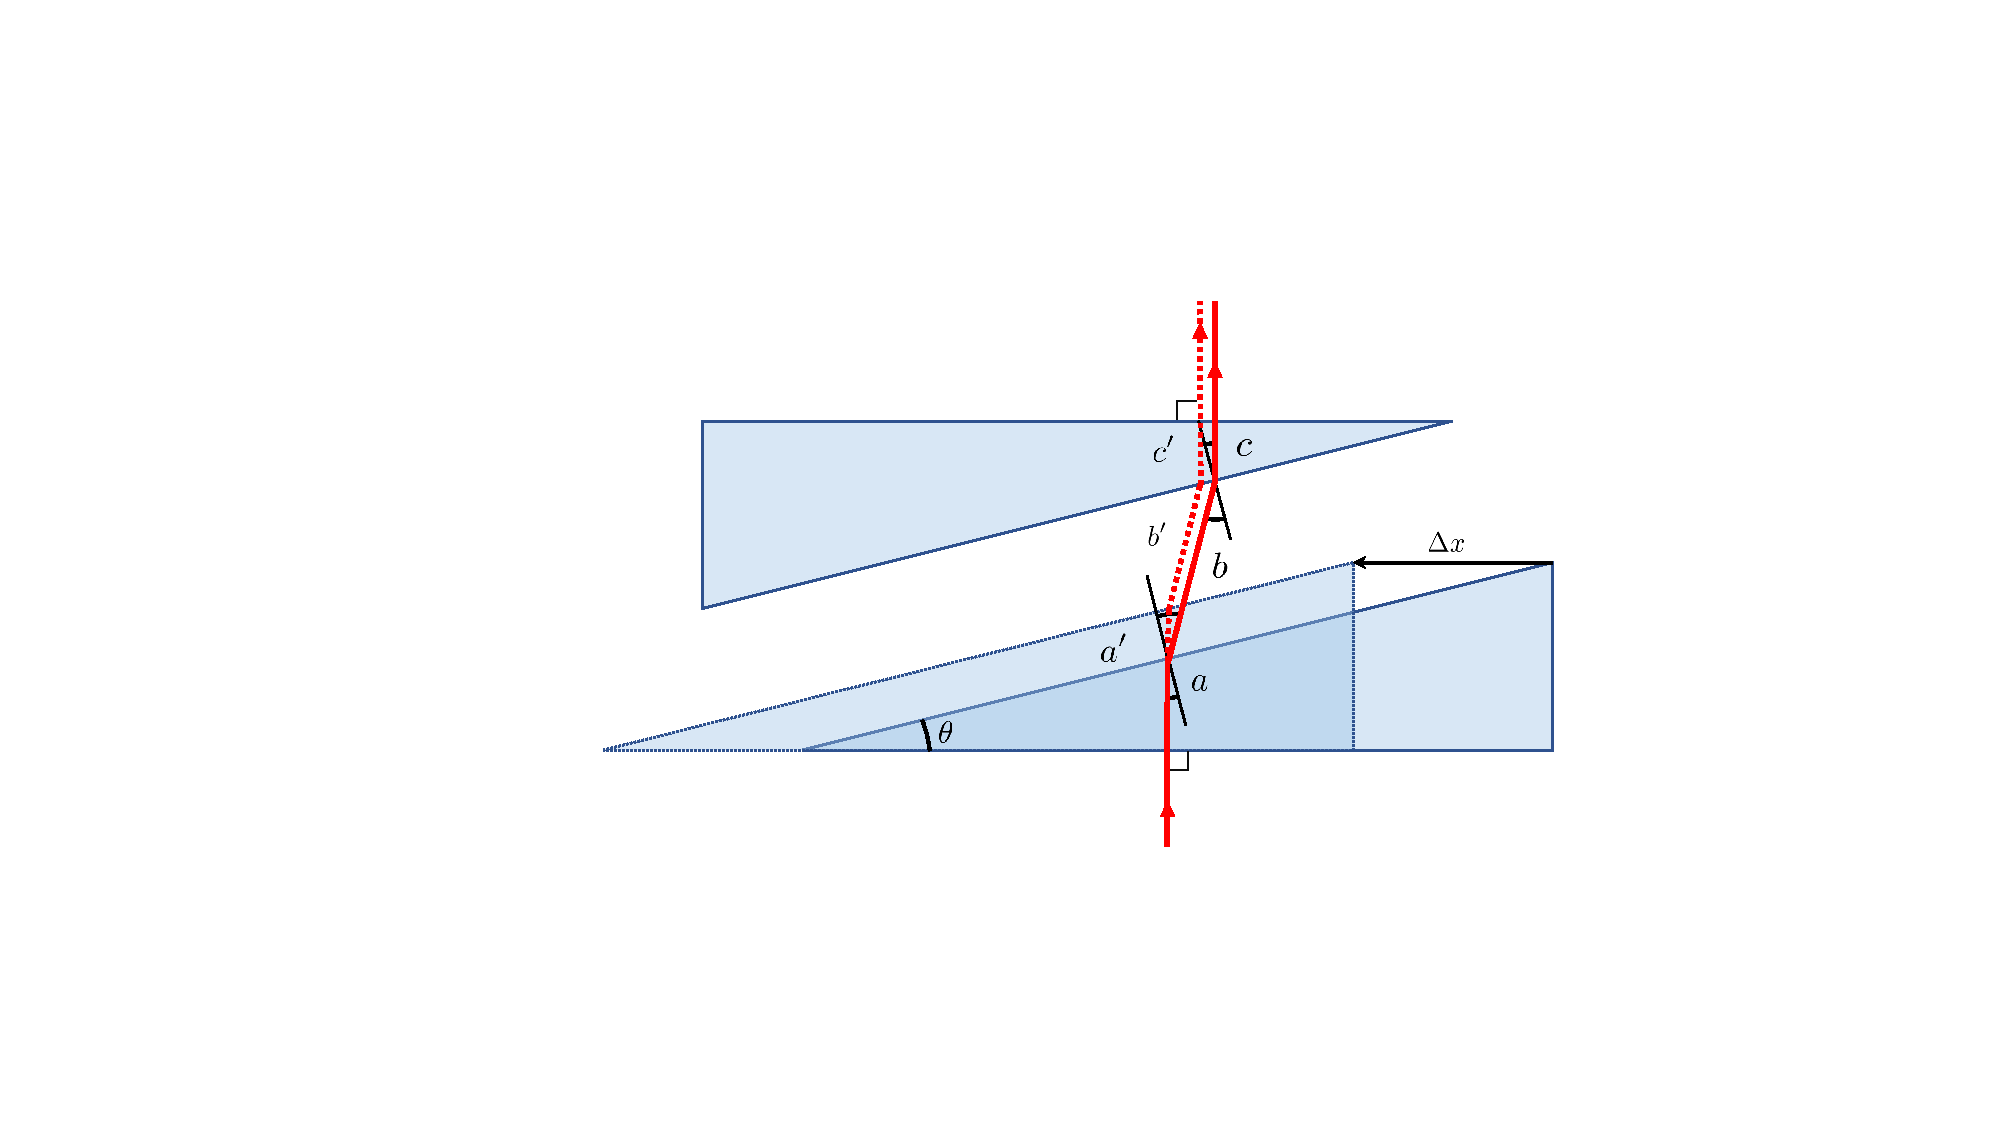
\includegraphics[width=0.6\textwidth]{figures/Beamline/wedge_delay_calibration.pdf}
	\caption[Schematic of FS wedges used for delay control]{Schematic of the FS wedges used to control the time delay between the IR and XUV pulses in the dressing and generation arms interferometer, respectively. The wedges are aligned such that the input beam is normal to the first wedge face, and the beam exits the wedges normal to the last face of the second wedge.  Only one of the wedges is motorized and is shown before and after a displacement by an amount $\Delta x$.}
	\label{fig:wedges}
\end{figure}

The second common method to control the delay between the pump and probe pulse is to use a pair of glass wedges \cite{chirlaAttosecondPulseGeneration2011, gormanAttosecondProbingElectron2018, kiesewetterDynamicsNearThresholdAttosecond2019}. A schematic of how this is achieved is shown in figure \ref{fig:wedges}.  In this scheme, only one of the glass wedges is motorized, and the direction of translation is perpendicular to the input beam and parallel to the first glass face.  The path that a ray would take through the wedge pair is shown before ($a\rightarrow b\rightarrow c$) and after ($a' \rightarrow b'\rightarrow c'$) translation by an amount $\Delta x$.  Assuming that the wedge angle is $\theta$, the path after translation by $\Delta x$ can be written as
\begin{align}
\label{eqn:path_lengths}
	a'&=a+\Delta x \tan\theta\\
	b'&=b-\Delta x \bigg(\frac{\sin\theta}{\cos\psi}\bigg)\\
	c'&=c+\Delta x \tan\theta\bigg(\frac{\sin(\psi-\theta)}{\cos\theta}\bigg)
\end{align}
where
\begin{equation}
	\psi = \arcsin(n\sin\theta)
\end{equation}
is given by Snell's Law \cite{pedrottiIntroductionOptics2007}. From the difference in optical path length between these two paths, one can calculate the time delay $\Delta\tau$ introduced by a translation of $\Delta x$, and this relationship is given by
\begin{equation}
\label{eqn:time_delay}
	\Delta\tau = \frac{\Delta x}{c}\Bigg[n\tan\theta - \frac{\sin\theta}{\cos\psi}-n\tan\theta\bigg(\frac{\sin(\psi-\theta)}{\cos\theta}\bigg)\Bigg].
\end{equation}
For a pair wedges made out of fused silica (Infrasil) with a wedge angle of $\theta=4^\circ$ and a beam of wavelength 1430 nm (n=1.4454), equation \ref{eqn:time_delay} becomes
\begin{equation}
\label{eqn:numerical_relationship_wedges}
	\Delta\tau = \Bigg(102 \bigg[\frac{\mathrm{as}}{\mathrm{\mu m}}\bigg]\Bigg)\Delta x.
\end{equation}
This entails that a translation of 1 $\mu$m would lead to a delay of only 100 as.  This reduction in motor step to delay step ratio compared to the retroreflector case means that the requirements on the motorized stage are greatly reduced.  Additionally, since the glass wedges are a transmissive optic, they are inherently less sensitive to vibrations when compared to a retroreflector.

In the TABLe apparatus, both types of delay control have been implemented, as shown in figure \ref{fig:beampath_sketch}.  The retroreflector is mounted on a translation stage with 2 inches of travel that is controlled manually with a micrometer.  The primary use for the retroreflector is to make coarse adjustments to the dressing arm to account for changes in temporal overlap between the two arms of the interferometer.  Typically, this is due to adjustments made to the interferometer itself (such as introducing new optics) or due to changes in the input laser, usually either pointing or wavelength.  

To finely control the delay, a pair of glass wedges is used.  These wedges are made out of fused silica, and have a wedge angle of $\theta=4^\circ$.  The first of the two wedges are motorized in manner similar to that shown in figure \ref{fig:wedges}.  The stage that the first wedge is mounted to has a total travel of 1 inch, and it is controlled by a Thorlabs Z825B DC servo motor.  This "pencil" motor, as it is known in the lab, has a minimum repeatable incremental motion of 0.2 $\mu$m and is encoded, so it's absolute position is known to within the homing accuracy of $\pm1$ $\mu$m.  From equation \ref{eqn:numerical_relationship_wedges}, using these wedges at 1430 nm with a step size of 1 $\mu$m will give a delay of 101 as.


\subsection{IR Dressing Intensity}
\label{sec:dressing_intensity}

An important consideration in any pump/probe experiment is the intensity of the IR field that is used as a probe/dressing field. Ideally, one would like to be able to control the intensity such that both perturbative and strong-field regimes can be accessed with the same optical setup.  This can be achieved by selecting an optical setup that has a high peak intensity and then attenuate the beam to achieve a lower intensity.  Attenuation can be achieved through the use of neutral density (ND) filters, however they can lead to several complications.  Since the ND filter would be placed in only one arm of the interferometer to control only the dressing intensity, any variation in thickness between different ND filters would lead to a change in temporal overlap.  Additionally, any change in positioning when switching ND filters will lead to a slight change in spatial overlap. In light of this, the method to attenuate the beam that was implemented in the TABLe interferometer is a half-wave plate (HWP) and a wire grid polarizer (WGP).  By rotating the polarization using the HWP, we can finely control the intensity  of the dressing field by using the WGP to transmit only one component of the rotated polarization.  The WGP is set such that the initial polarization is maintained, and this insures that the polarization of the IR and XUV are parallel in the interaction region.  A second WGP is used to increase the effective extinction ratio to ensure that the field is linearly polarized even when it is being strongly attenuated.  The extinction ratio of one of the WGP (Thorlabs WP25M-UB) is approximately 12500:1 at 1430 nm.  Using this setup in conjunction with a beam splitter that reflects 8\% of the input energy to the dressing arm, the pulse energy can be tuned between 1 $\mu$J and 125 $\mu$J.

\begin{figure}
	\centering
	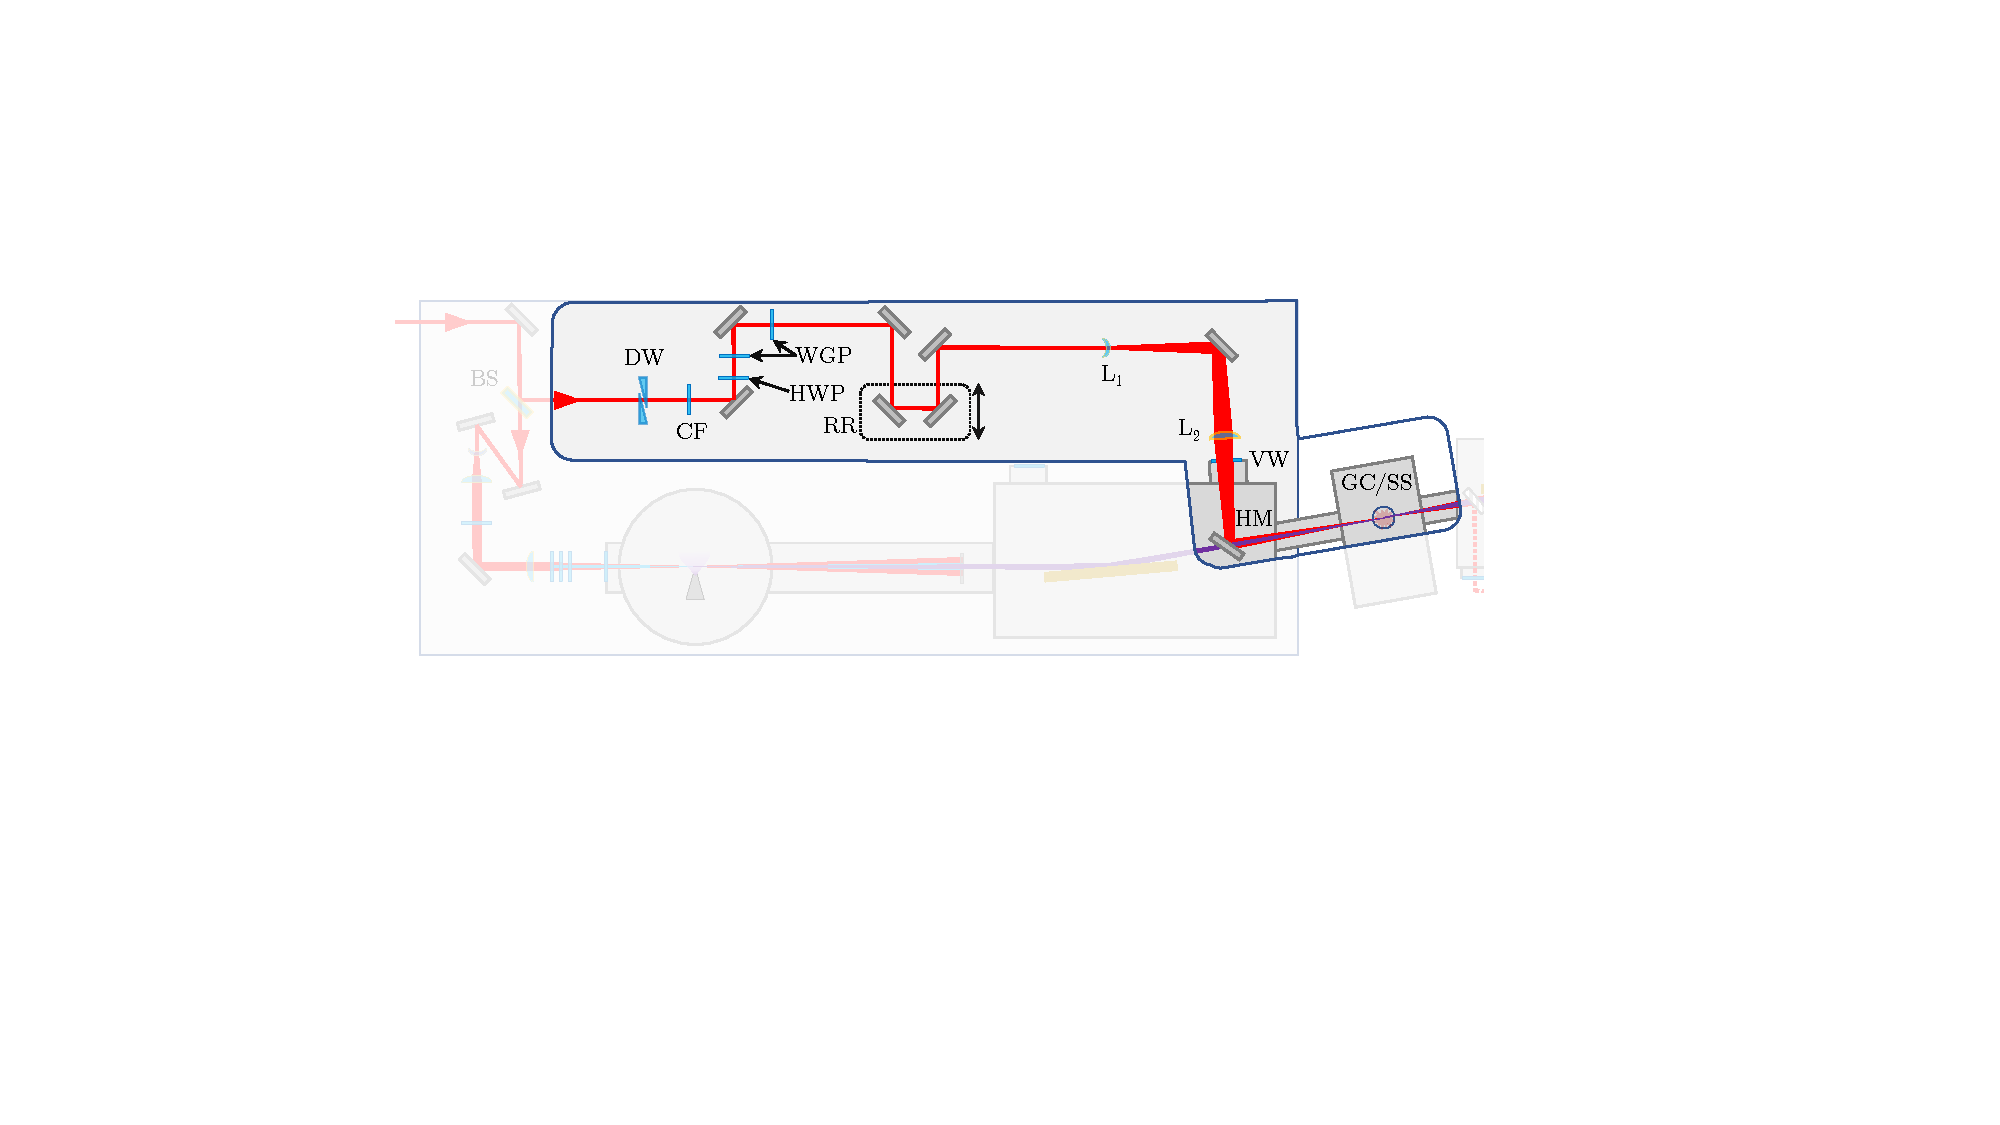
\includegraphics[width=0.9\textwidth]{figures/Beamline/dressing_arm.pdf}
	\caption[Optical layout of dressing arm]{Optical layout of the dressing arm of the TABLe interferometer. HWP and WGP are used to finely control the power in the dressing arm.  The lenses L$_1$ and L$_2$ were chosen to achieve a high intensity at the focal plane in the target chamber.  This was done to have the capability to drive strong-field processes in a gas medium \cite{kiesewetterDynamicsNearThresholdAttosecond2019}.  See figure \ref{fig:beampath_sketch} for full details of the interferometer.}
	\label{fig:dressing_arm}
\end{figure}

The next design consideration for the dressing arm of the interferometer is choosing focusing optics to set the peak intensity that is achievable at the interaction region.  The two main options in this regard are either focusing mirrors or lenses.  Focusing mirrors have a significant advantage in the fact that they are achromatic, however their use leads to an optical system that is generally larger in optical path length and is difficult to switch between focal geometries. Lenses in that regard are well suited to adjusting between different experimental configurations without changing the overall footprint of the interferometer.  The dressing lenses that are used in all of the experiments in this dissertation are shown in \ref{fig:dressing_arm}, and they were originally selected to achieve the highest possible intensity at the focal plane given the geometrical constraints of the TABLe \cite{kiesewetterDynamicsNearThresholdAttosecond2019}. This choice of lenses was made to drive strong-field processes in rare gas atoms in the interaction region, and they were selected based upon calculations done by D. Kiesewetter using a hole mirrors as both beam splitters in the interferometer \cite{kiesewetterDynamicsNearThresholdAttosecond2019}. His calculations estimated that the peak intensity at 1300 nm was 0.59 TW/cm$^2$ for a pulse energy of 1 $\mu$J just before L$_1$ in figure \ref{fig:dressing_arm}.

\begin{sidewaysfigure}%[ht]
	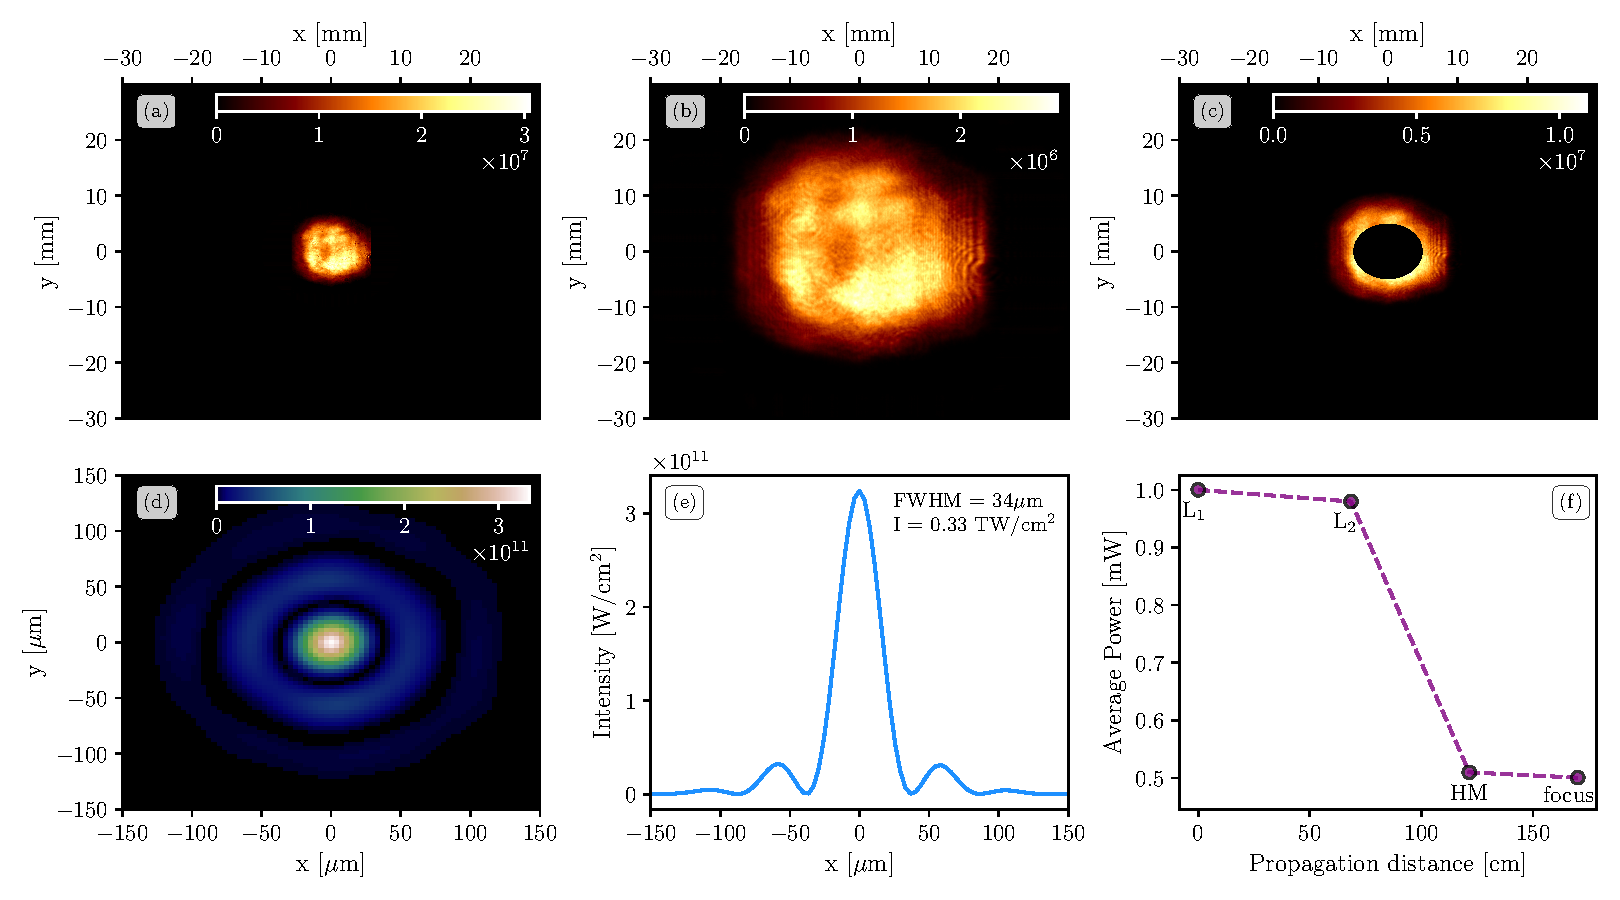
\includegraphics[width=\textwidth]{figures/Beamline/pump_intensity_profiles_1430nm_1uj.pdf}
	\caption[Calculation of dressing intensity]{(a) Beam profile of the signal from the TOPAS pumped by the Spitfire laser system.  Wavelength is 1430 nm and the pulse is normalized to 1 $\mu$J of pulse energy.  Beam profile was measured using a thermal camera, and is used as the input to the beam propagation simulation that is initiated just before L$_1$ in figure \ref{fig:dressing_arm}. (b) Numerically propagated beam profile just after L$_2$ in figure \ref{fig:dressing_arm}. (c) Beam profile just after reflecting off the hole mirror.  (d) Calculated intensity profile at the focal plane in the interaction region. (d) Lineout of the calculated intensity profile.  For an input pulse energy of 1 $\mu$J, a peak intensity of 0.33 TW/cm$^2$ can be achieved.  (f) Integrated average power at different point in the calculation.  The main source of energy loss is due to the hole mirror, which only reflects 52\% of the incident light.  The hole mirror has an inner radius of 5 mm in this case.}
	\label{fig:dressing_intensity}
\end{sidewaysfigure}


For the experiments described herein, the initial beam splitter was changed to a beam sampler, and the recombining hole mirror was changed to a hole diameter of 10 mm from 6 mm.  This was done to maximize the XUV flux by sending as much energy to generation as possible while minimizing clipping of the XUV with the hole mirror.  In light of these changes, it is important to determine what the new peak intensity is at the focus.  To accurately determine the intensity, a beam propagation simulation is performed using the measured beam profile.  It is important to use the measured beam profile because the spatial mode out of the TOPAS is decidedly non-Gaussian, and this can be seen in figure \ref{fig:dressing_intensity} (a) which shows the beam profile at 1430 nm measured on a thermal camera.  Beam propagation is implemented using an open-source Python package developed by Flexible Optical B.V. (OKO Tech) called LightPipes.  The package consists of numerical methods to calculate the Fresnel integral
\begin{equation}
\label{fresnel_integral_0}
u(x,y,z)=\frac{i k}{2\pi z}e^{i k z}e^{i k (x^2+y^2)/2z}\int_{-\infty}^{\infty}\int_{-\infty}^{\infty}u(\xi,\eta,0) e^{ik(\xi^{2}+\eta^{2})/2z} e^{-ik(x\xi + y\eta)/z} \diff\xi\diff\eta
\end{equation}
which gives the field $u(x,y,z)$ after propagation of a distance $z$, given an initial field profile of $u(x,y,0)$.  Using this formalism, a thin lens of focal length can be treated as adding a quadratic phase $\phi=-\pi(x^2+y^2)/\lambda f$ to the field, and the effect of apertures can also be included to account for the effect of diffraction on the beam profile and intensity \cite{goodmanIntroductionFourierOptics2005}.

The results of the simulation are shown in figure \ref{fig:dressing_intensity}.  This simulation was performed for an input pulse energy of 1 $\mu$J at a wavelength of 1430 nm. The simulation begins just before L$_1$ in \ref{fig:dressing_arm} and the beam is propagated through to the interaction region GC/SS.  The beam profile at L$_2$ and immediately after the hole mirror is shown in figure \ref{fig:dressing_intensity} (b) and (c), and the intensity profile at the focus is shown in figure \ref{fig:dressing_intensity} (d).  From these simulations, the peak intensity for a pulse energy of 1 $\mu$J is 0.33 TW/cm$^2$. For the range of pulse energies available in the dressing arm, this corresponds to an intensity range of 0.33 - 41.3 TW/cm$^2$ that is achievable.

\subsection{XUV Beam Size}
\label{sec:xuv_beam_size_knife_edge}

Another important consideration in any pump/probe experiment is the beam size of the probe relative to the pump in the interaction region.  The reason for this is because the probe beam inherently samples the excited state of the system induced by the pump at intensities within the intersection of the pump and probe focal volumes contained within the system being studied.  Thus, a smaller probe waist relative to the pump waist means that a narrower distribution of pump intensities will be sampled by the XUV probe.  The width of this distribution limits the ability to study intensity dependent effects, and it is a critical parameter to control. As stated previously, the demagnification of the XUV spot size provided by the ellipsoidal mirror helps tremendously to achieve as small ratio of probe to pump beam sizes even at small pump beam sizes that are used.

Additionally, it is also of great importance to place the sample at the focus of both the XUV and the IR beams in the target chamber.  This can be done easily with the IR either through direct imaging of the beam or by using an intensity dependent effect (such as second harmonic generation from a BBO) to find the peak intensity along the k-direction of the IR beam.  The focus of the XUV is more difficult to find because it must be found in vacuum.  One method to find the focus is to measure the beam diameter at various points along the k-direction of the XUV to find the minimum beam diameter.  A method to do this is to employ a knife-edge measurement \cite{arnaudTechniqueFastMeasurement1971, skinnerMeasurementRadiusHighpower1972,marshallTwoMethodsMeasuring2010,almeidaHarmonicsBeamsCharacterization2016}.

\begin{figure}
	\centering
	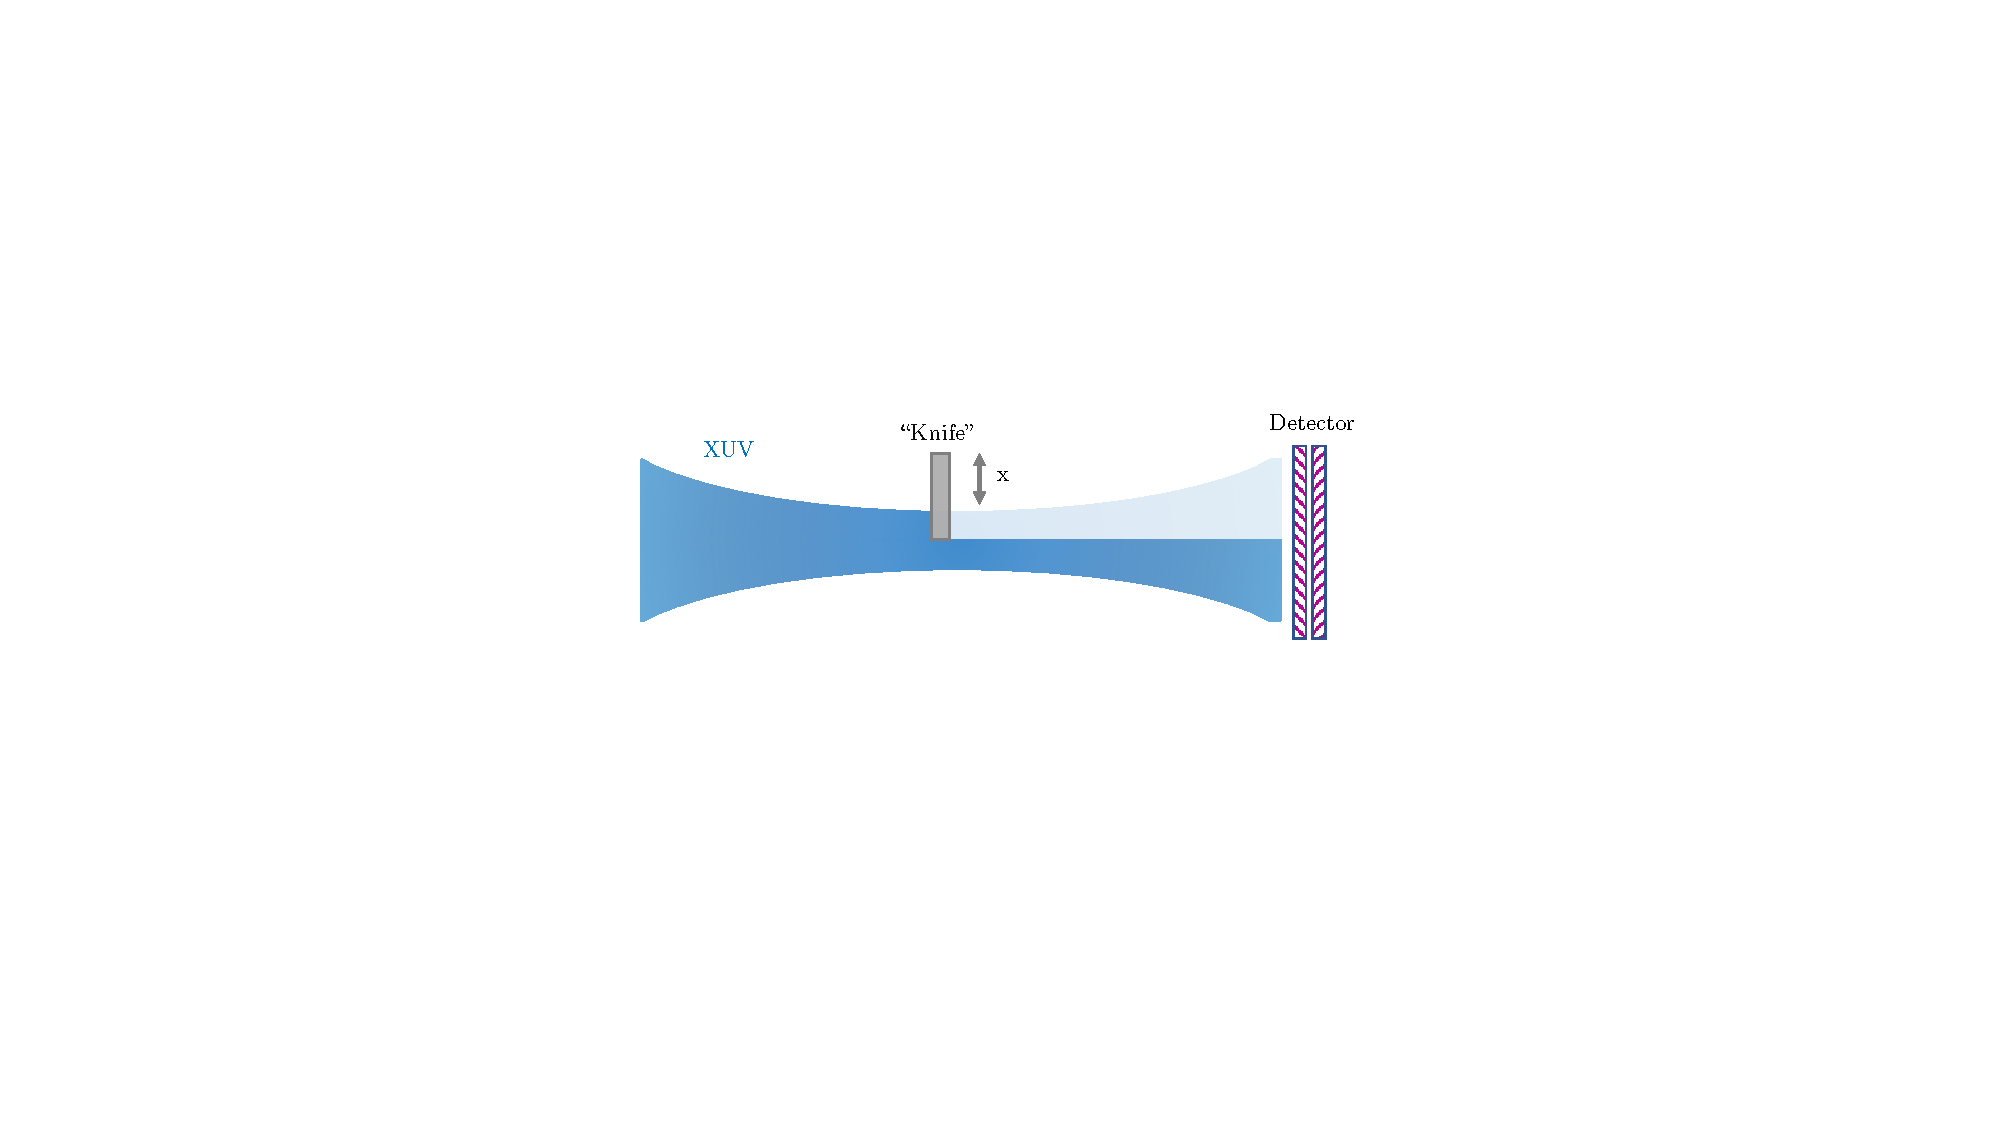
\includegraphics[width=0.7\textwidth]{figures/Beamline/knife_edge_xuv.pdf}
	\caption[Schematic of knife-edge technique to measure beam size]{Schematic of knife-edge technique to measure beam size. By translating a sharp beam block through the focus and measuring the total transmitted power the beam profile can be reconstructed.}
	\label{fig:knife_edge_beam_size_measurement}
\end{figure}

The principle behind the knife-edge measurement is simple, and it is shown schematically in figure \ref{fig:knife_edge_beam_size_measurement}.  In the measurement, a "knife" is translated through the beam to be measured perpendicular to the k-direction of the beam.  The knife is simply an opaque material that has a sharp edge to minimize scattered light.  As this knife is translated through the focus, the total power is measured further downstream as a function of the knife's position within the beam, and this dependence is given by
\begin{equation}
	\label{eqn:knife_edge_power}
	P(x,z) = \int_{-\infty}^{\infty}\int_{-\infty}^{x}I(x', y',z)\diff y\diff x'
\end{equation} 
where $I(x,y,z)$ is the intensity of the beam.  For a Gaussian beam, this relationship becomes
\begin{equation}
	\label{eqn:knife_edge_power_guassian}
	P(x,z) = \frac{P_0}{2}\mathrm{erfc}\bigg(\frac{x\sqrt{2}}{w(z)}\bigg)
\end{equation}
where $w(z)$ is waist radius as a function of $z$ and is given by
\begin{equation}
	\label{eqn:gaussian_waist_radius}
	w(z)=w_0\sqrt{1+\bigg(\frac{z - z_0}{z_R}\bigg)^2}
\end{equation}
where $z_R=\pi w_0^2 n/\lambda$ is the Rayleigh range and $z_0$ is the position of the focus along the k-direction. 

An example of this technique being used to measure the beam size of the XUV is shown in figure \ref{fig:xuv_beam_size}.  In this case, the knife being used is the beveled edge of a silicon frame that is 300 $\mu$m thick. The thickness of the frame is such that the transmission is negligible through the frame itself.  The integrated harmonic signal is fit to
\begin{equation}
	P(x) = \frac{a}{2}\mathrm{erfc}\bigg(\frac{\sqrt{2}(x-x_0)}{w}\bigg) + b,
\end{equation}
and the beam size can be extracted from the fit.  In this case the beam size was 9 $\mu$m at this position of the XUV focus.  Comparing this beam size to the predicted beam size of the IR, we can see that the XUV spot size relative to the IR spot size is roughly three times smaller.

\begin{figure}
	\centering
	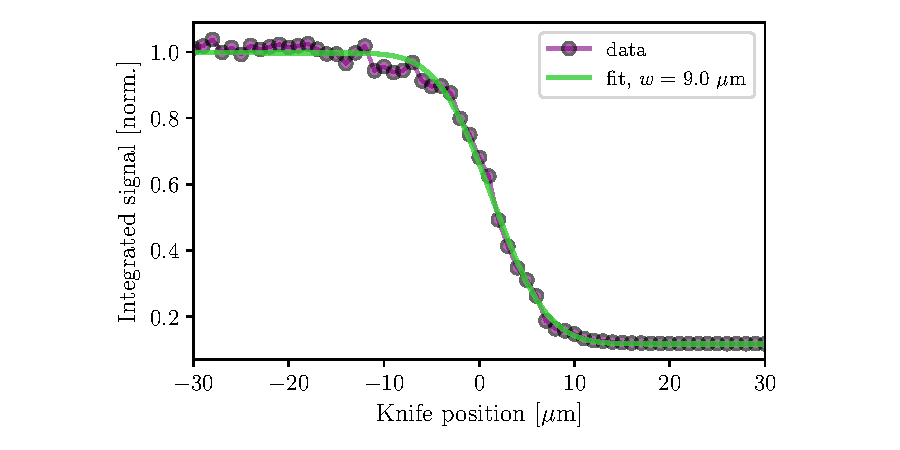
\includegraphics[width=0.9\textwidth]{figures/Beamline/integrated_knife_edge_xuv.pdf}
	\caption[Schematic of knife-edge technique to measure beam size]{Schematic of knife-edge technique to measure beam size. By translating a sharp beam block through the focus and measuring the total transmitted power the beam profile can be reconstructed.}
	\label{fig:xuv_beam_size}
\end{figure}


This measurement can repeated along the k-direction of the XUV beam, and the focus can be mapped out.  An example of this type of measurement is shown in figure \ref{fig:xuv_focus}.  As can be seen, the fit to a Gaussian agrees quite well with the measure dependence of the beam profile.  The extracted Rayleigh range is 1.1 mm with a waist of 6.1 $\mu$m at a motor position of 12.7 mm along the k-direction.  This type of measurement is performed whenever the optical setup is changed in the generation arm of the interferometer, as it insures that the sample is always at the focus of the XUV.
\begin{figure}
	\centering
	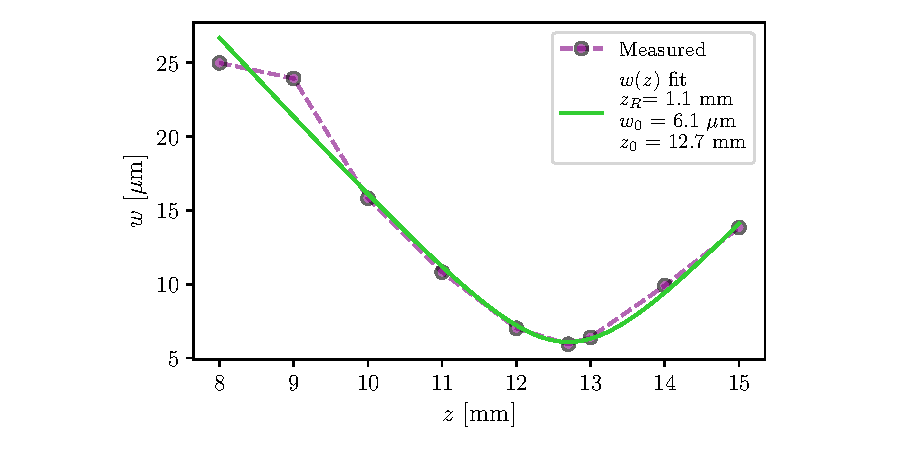
\includegraphics[width=0.9\textwidth]{figures/Beamline/xuv_focus.pdf}
	\caption[Finding focus of XUV using knife-edge measurements]{Focus of the XUV measured using knife-edge method at various points along the k-direction of the XUV beam.}
	\label{fig:xuv_focus}
\end{figure}


\section{Conclusion}

In this chapter the design and optical layout of the Transient Absorption Beamline (TABLe) was described.  This experimental apparatus represent the culmination of years of design, construction, and validation performed by Greg Smith and myself.  The unique capabilities of the TABLe enabled the work detailed in this dissertation to be performed, as well as other experiments \cite{kiesewetterDynamicsNearThresholdAttosecond2019, camperHighRelativephasePrecision2019, leshchenkoHighpowerFewcycleCr2020}.
%\section{Spectrometer Calibration}
%\label{subsec:spec_calibration}

%\begin{figure}
%	\centering
%	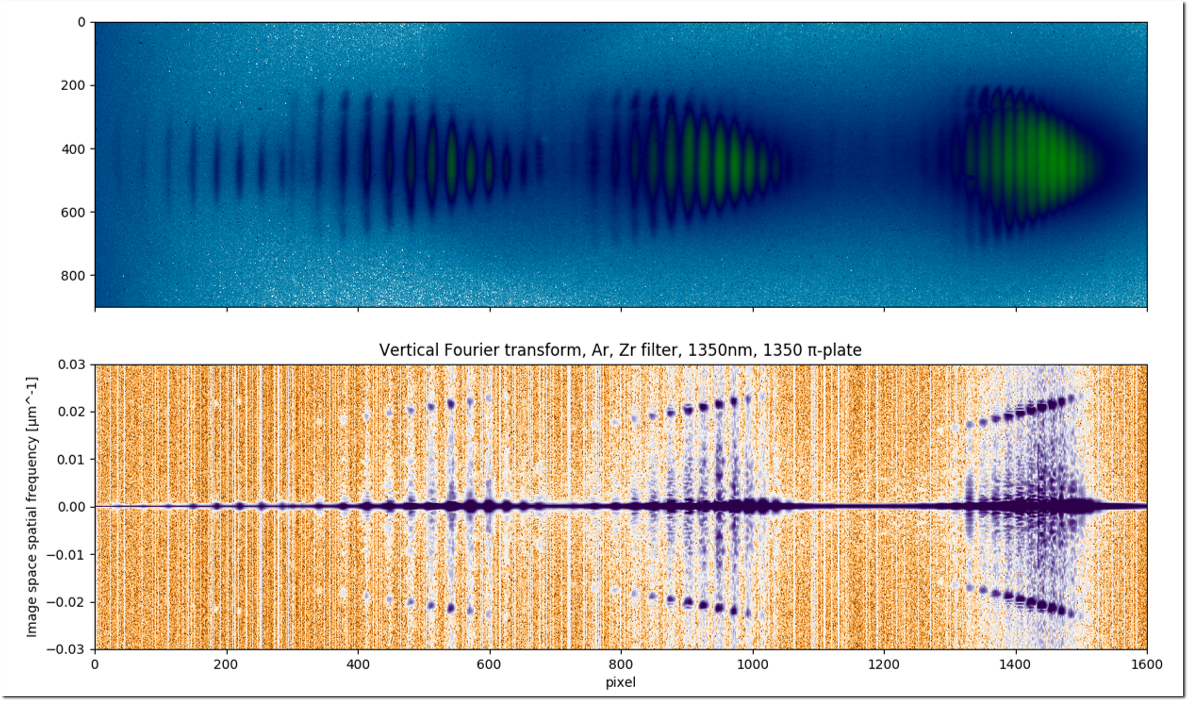
\includegraphics[width=0.9\textwidth]{figures/Beamline/first_to_third_order_diffraction.png}
%	\caption{INCOMPLETE: multiple diffraction orders}
%	\label{fig:first_to_thirds_order}
%\end{figure}

%\begin{figure}
%	\centering
%	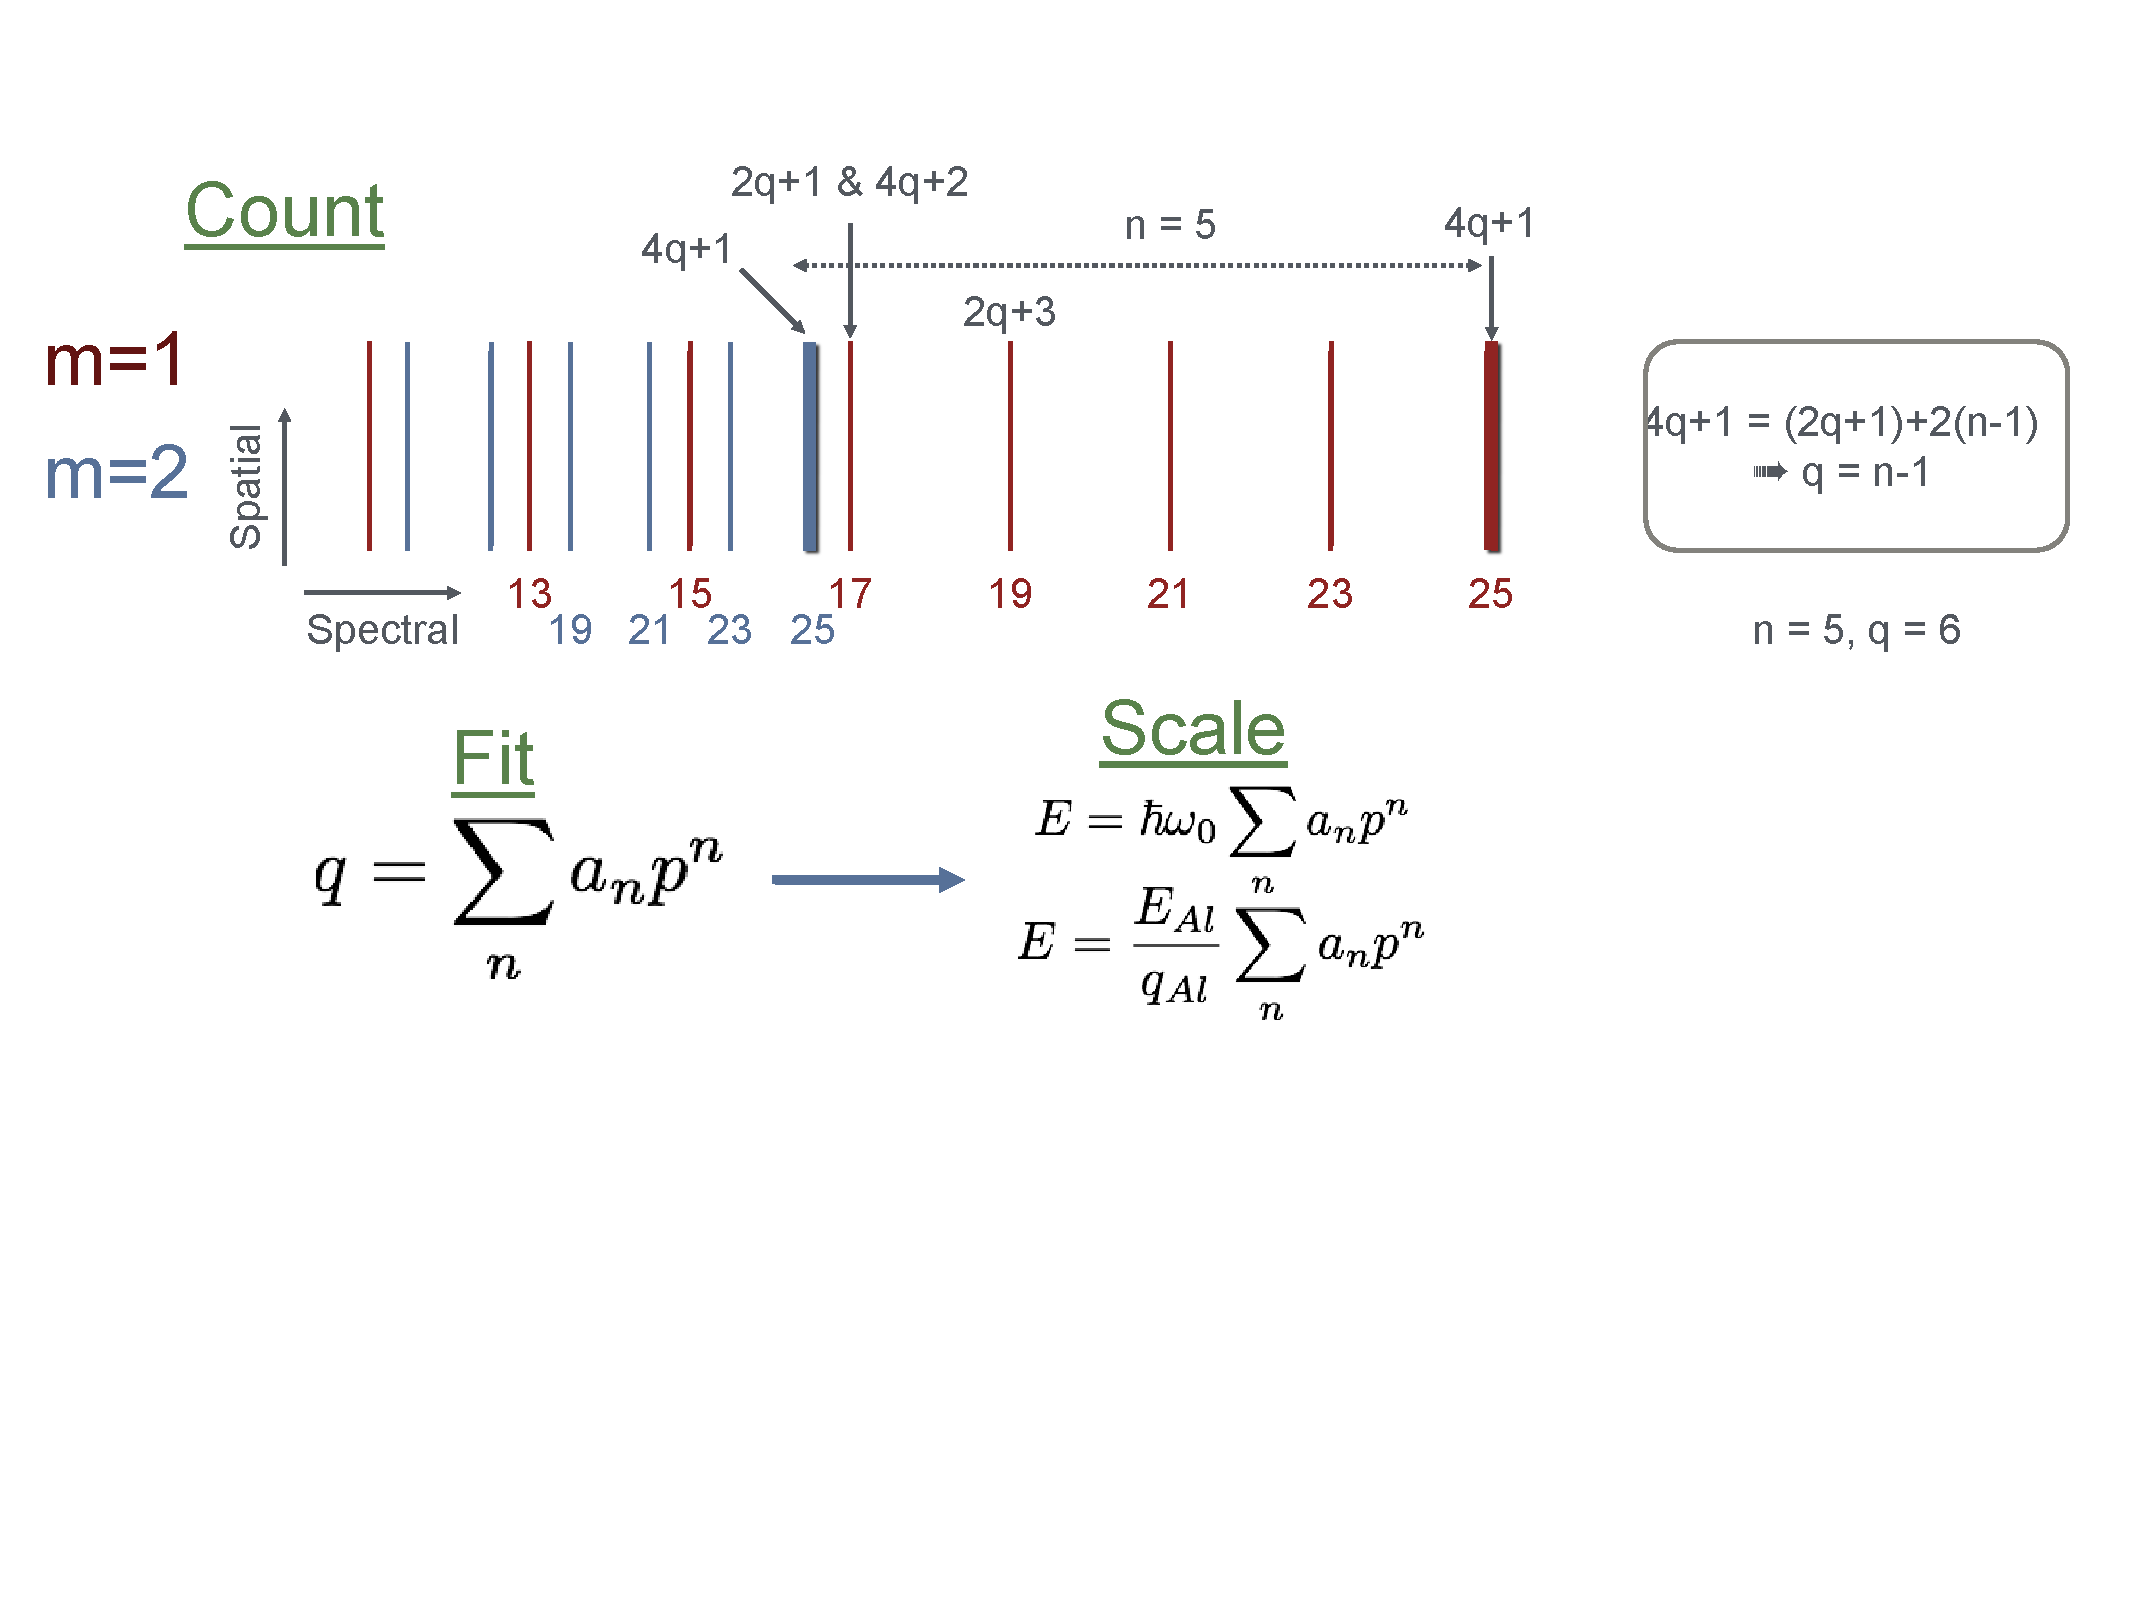
\includegraphics[width=0.9\textwidth]{figures/Beamline/Count_Fit_Scale.pdf}
%	\caption{INCOMPLETE: count fit scale scheme}
%	\label{fig:count_fit_scale_scheme}
%\end{figure}

%\begin{figure}
%	\centering
%	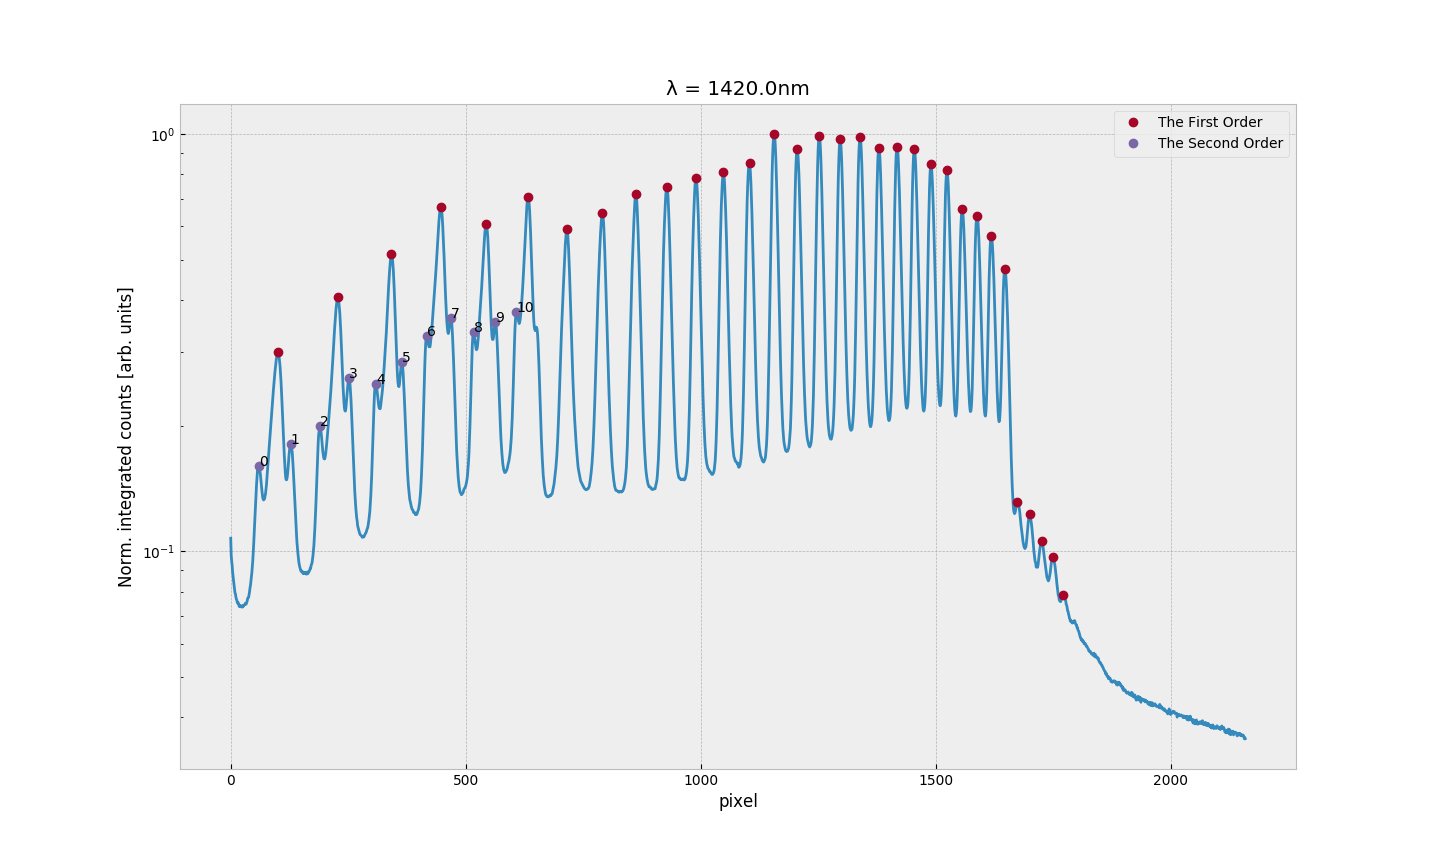
\includegraphics[width=0.9\textwidth]{figures/Beamline/first_second_order_spectrum.png}
%	\caption{INCOMPLETE: multiple diffraction orders}
%	\label{fig:first_second_order}
%\end{figure}

%\begin{figure}
%	\centering
%	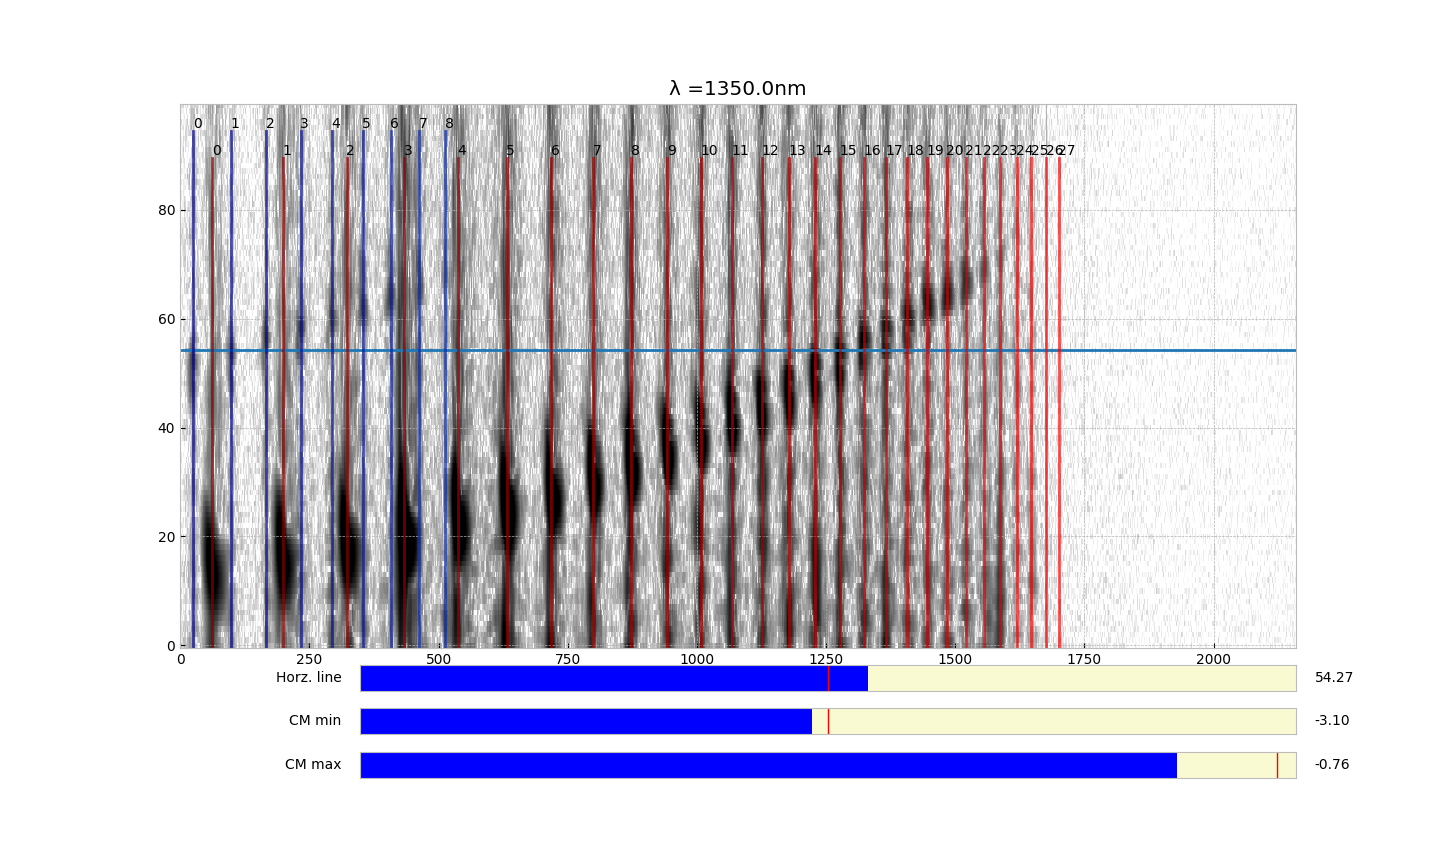
\includegraphics[width=0.9\textwidth]{figures/Beamline/line_matching_first_and_second.png}
%	\caption{INCOMPLETE: line matching}
%	\label{fig:line_matching}
%\end{figure}

%\begin{figure}
%	\centering
%	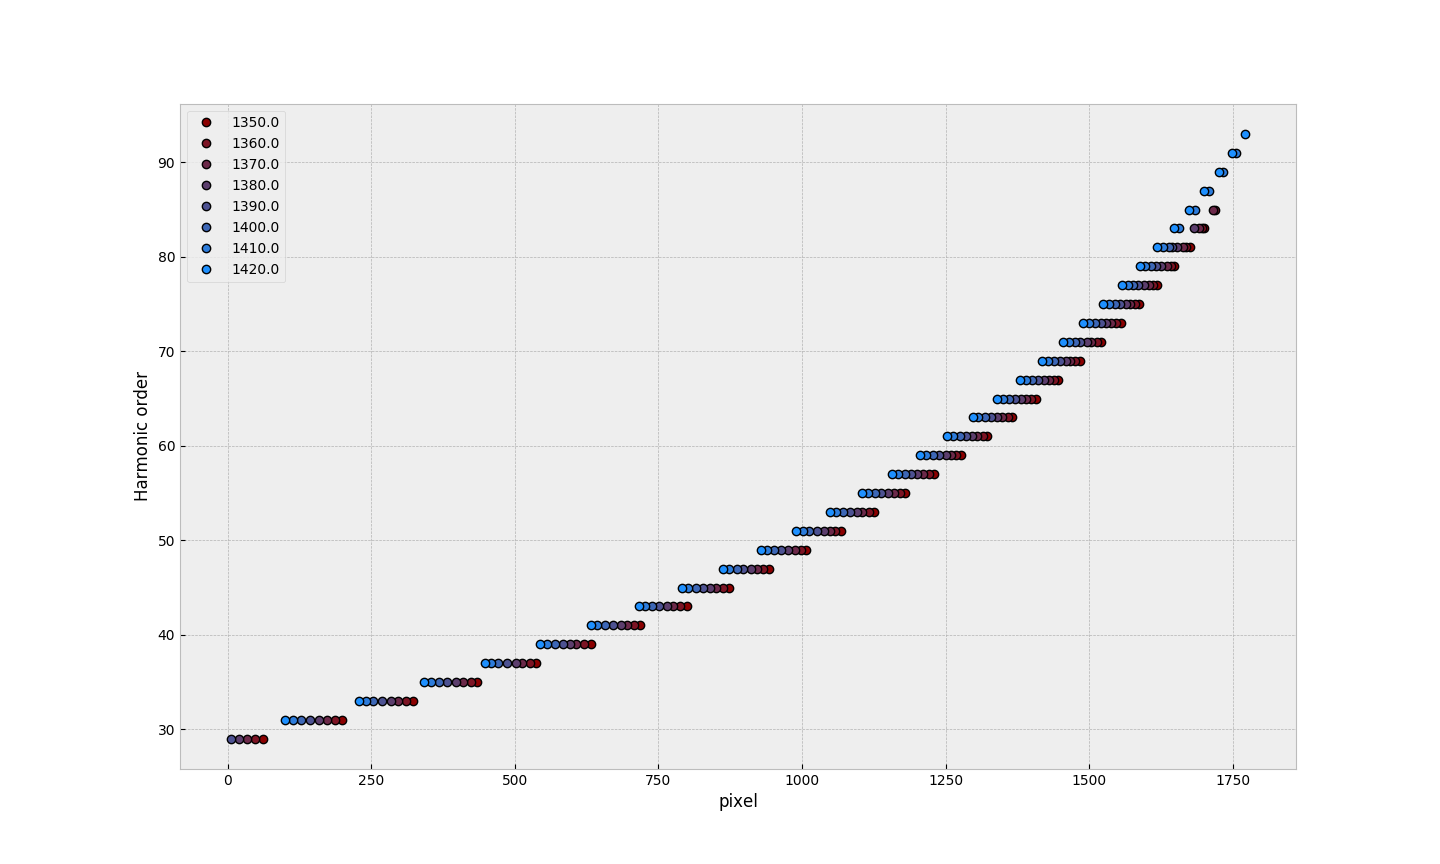
\includegraphics[width=0.9\textwidth]{figures/Beamline/harmonic order vs pixel.png}
%	\caption{INCOMPLETE: harmonic order vs pixel}
%	\label{fig:harm_order_vs_pixel}
%\end{figure}

%\begin{figure}
%	\centering
%	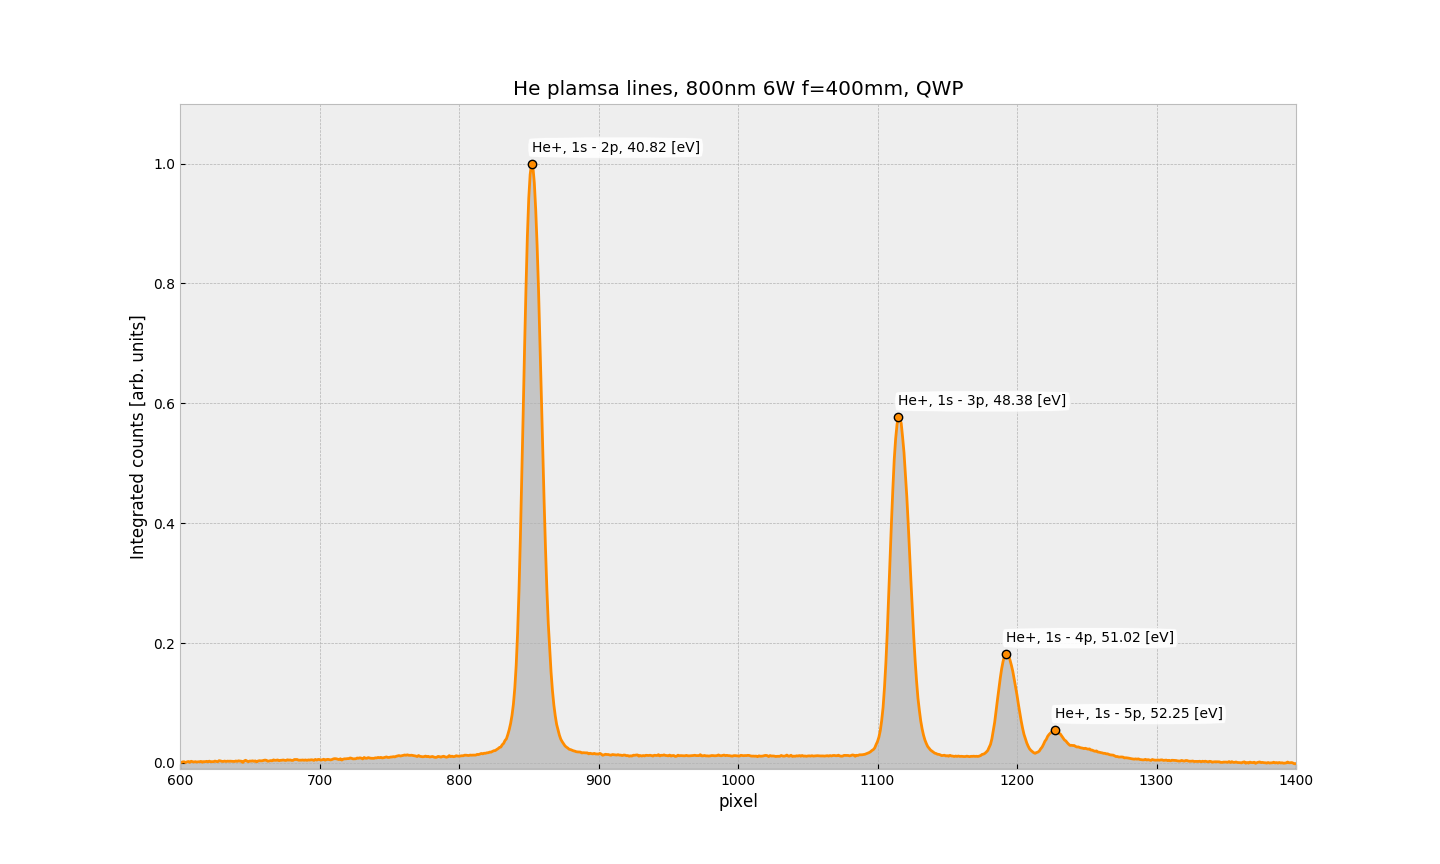
\includegraphics[width=0.9\textwidth]{figures/Beamline/He_plasma_line_spectrum.png}
%	\caption{INCOMPLETE: he plasma lines}
%	\label{fig:He_plasma_lines}
%\end{figure}

%\begin{figure}
%	\centering
%	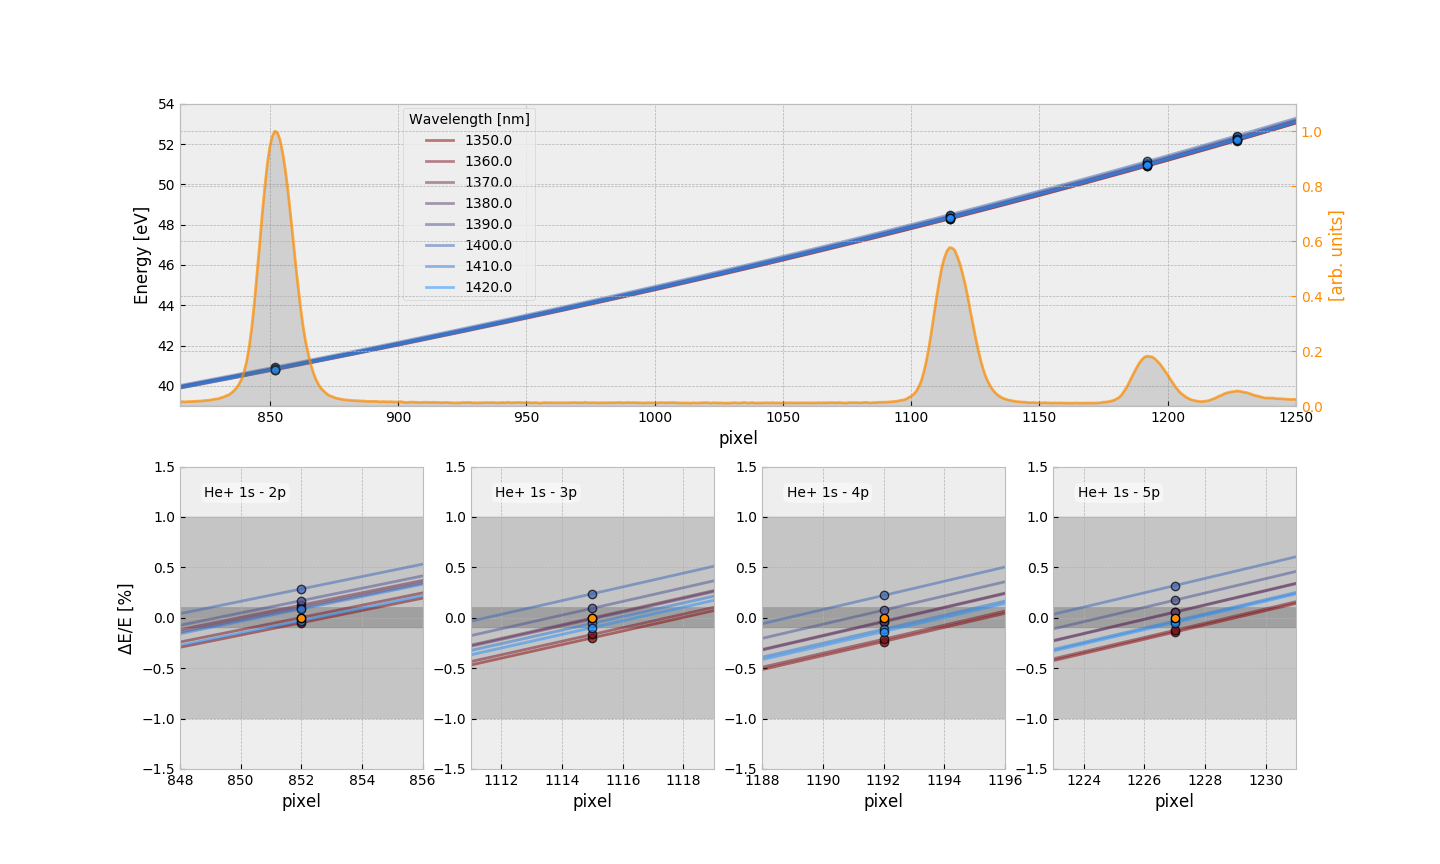
\includegraphics[width=0.9\textwidth]{figures/Beamline/He_plamsa_line_comparison.png}
%	\caption{INCOMPLETE: he plasma lines comparison}
%	\label{fig:plamsa_line_comparison}
%\end{figure}




%\chapter{Transient absorption of argon: Fano resonances}
\label{ar_fano_exp}

\section{Introduction}
\label{intro_ar_fano}

\lipsum
%\chapter{Two-source transient absorption spectroscopy}
\label{tatas}

\section{Introduction}
\label{intro_tatas}

\section{Theory}
\label{TsATAS_theory}


\section{Experiment}
\label{TsATAS_exp}

\begin{figure}
	\centering
	\includegraphics[width=0.9\textwidth]{figures/Two_source/dOD_dn.pdf}
	\caption{Camera image of two sources generating a filament in a gas cell. Image was taken while chamber was vented and at ambient pressure.}
	\label{my_anita}
\end{figure}
%\begin{appendices}
%\chapter{Square-wave Phase Grating}



           

%\chapter{HE-TOPAS Alignment}
\label{TOPAS}




\section{Introduction}
\label{intro_TOPAS}

\begin{figure}
	\centering
	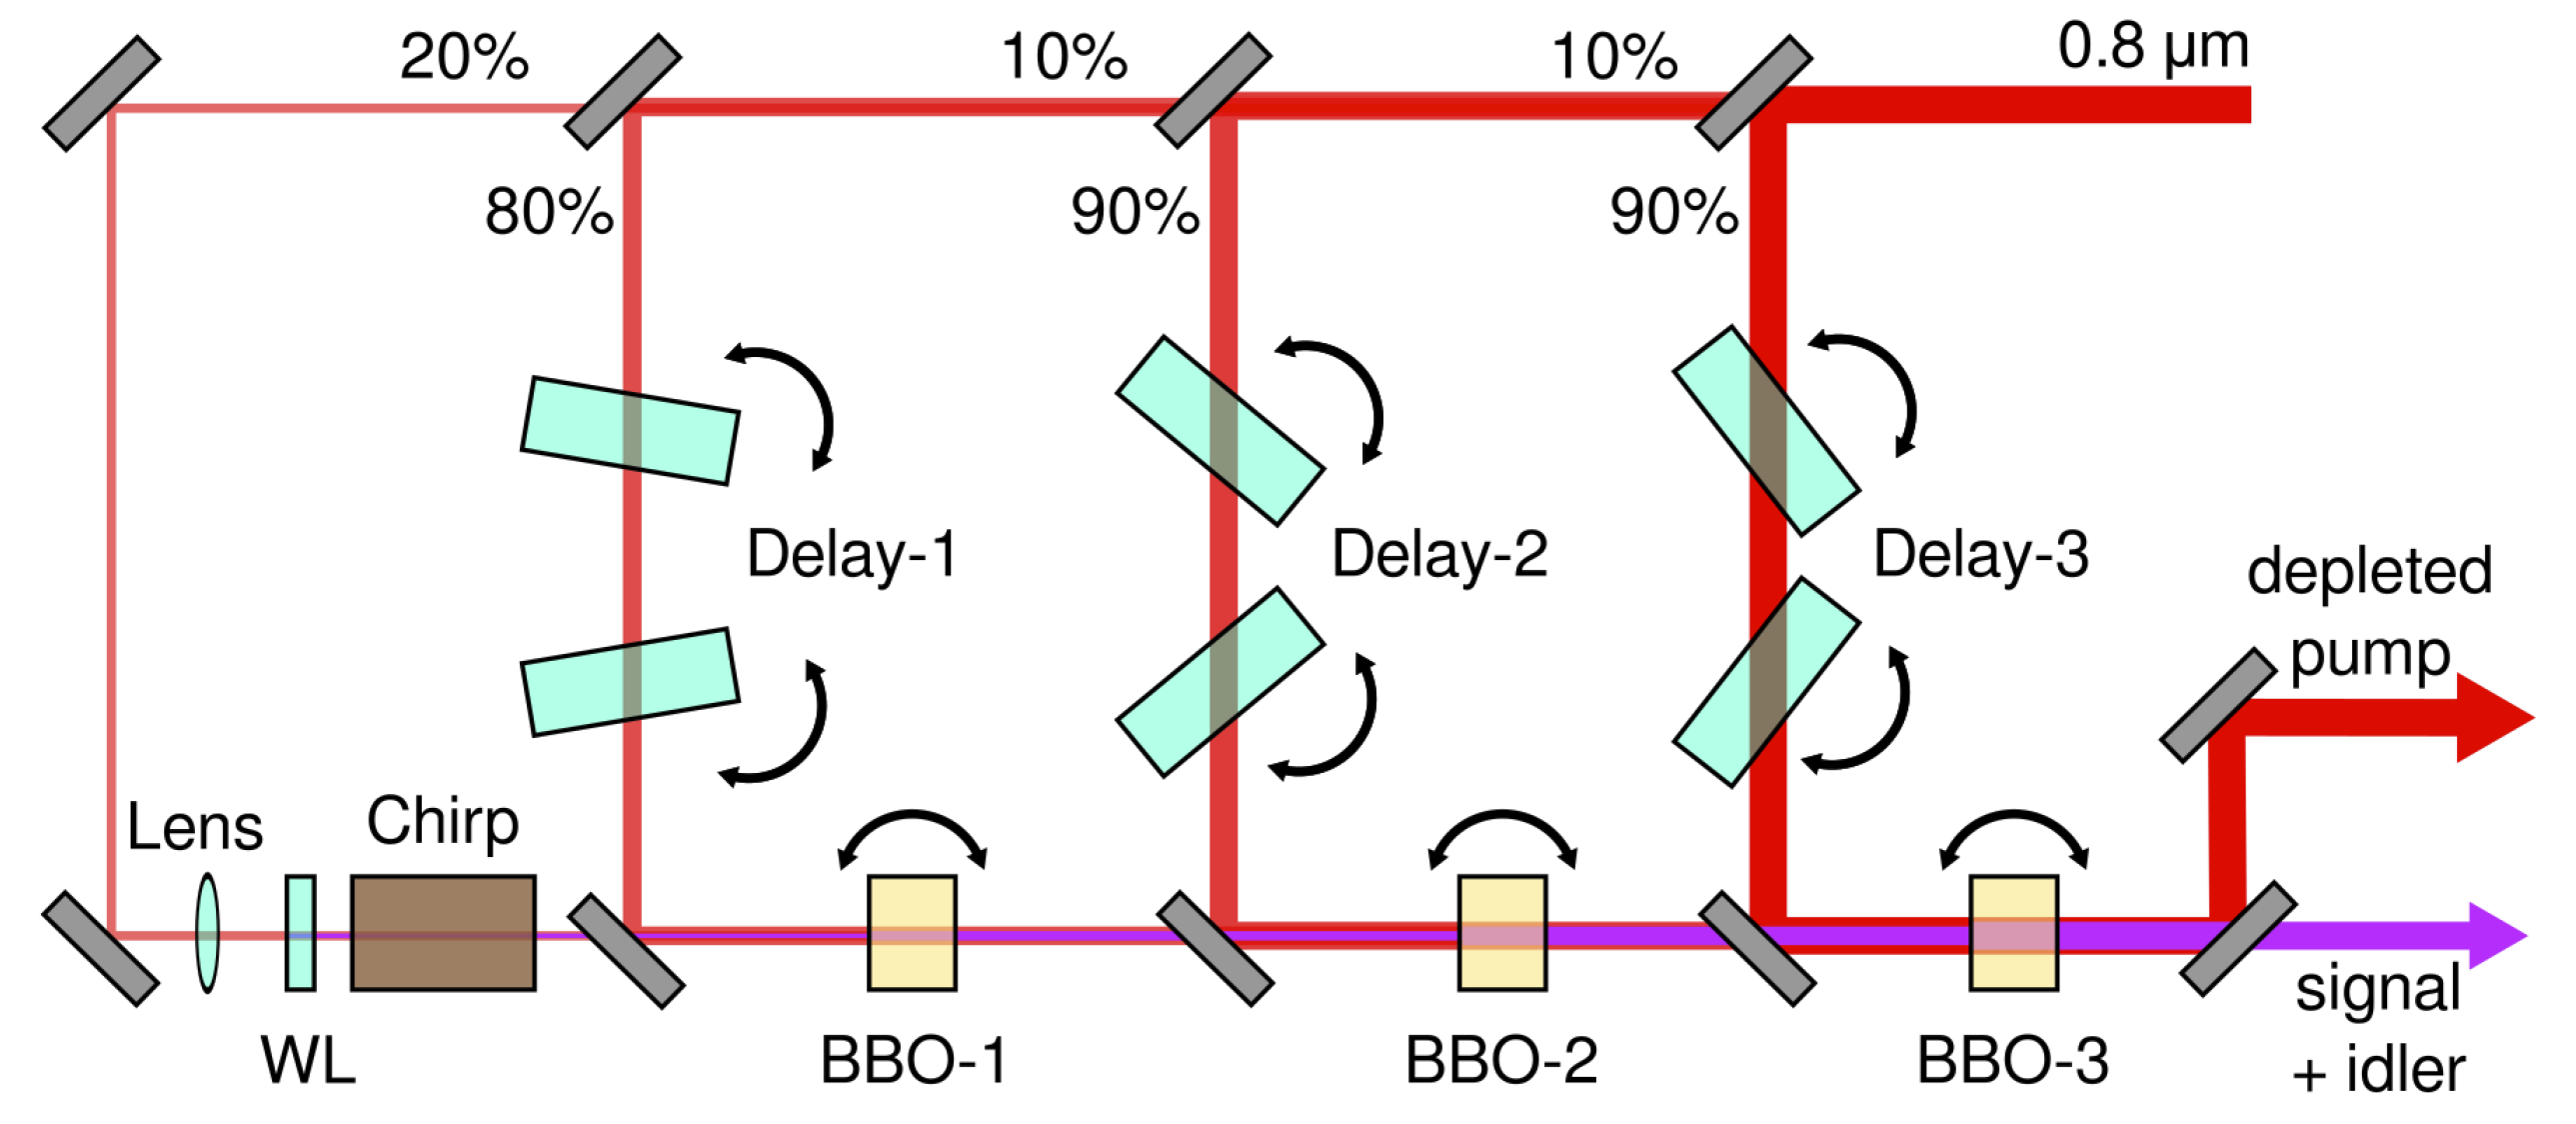
\includegraphics[width=0.9\textwidth]{figures/TOPAS/topas_cartoon.png}
	\caption{Cartoon diagram of the TOPAS layout. Adapted from....}
	\label{TOPAS_cartoon}
\end{figure}

\begin{figure}
	\centering
	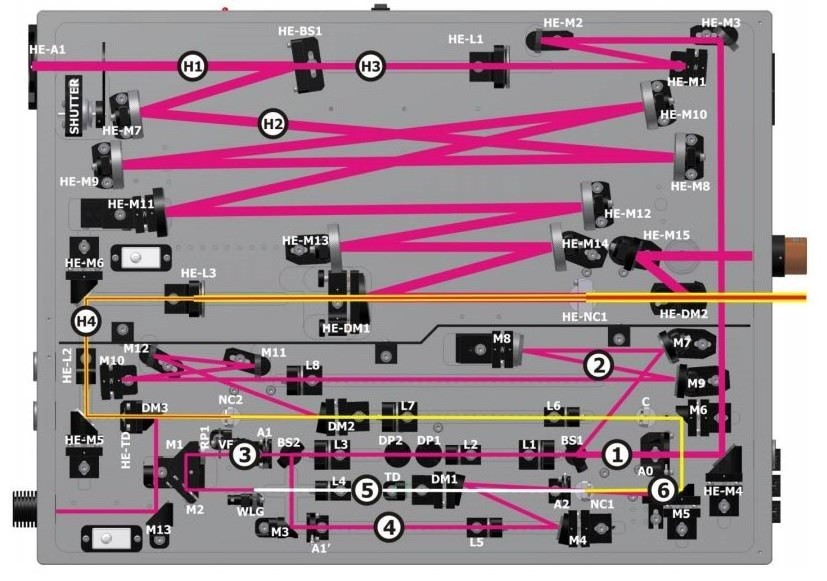
\includegraphics[width=0.9\textwidth]{figures/TOPAS/schematic_lightcon.jpg}
	\caption{Schematic of the TOPAS layout. Adapted from TOPAS manual.}
	\label{TOPAS_schematic}
\end{figure}
%\end{appendices}

\backmatter
% We use BIBTeX for the bibliography---you don't have to
%\nocite{*} % To display all refs, even uncited refs (useful when editting)
\bibliography{dissbib}
\bibliographystyle{unsrt} % use your favorite BIBTeX style

% If for some reason you are anti-BIBTeX, then you would use the
% following instead of the above:
%\begin{thebibliography}{99}
% ...
%\end{thebibliography}


% Note: GS 2010 requires bibliography/references _before_ the appendix
% if you believe their guidelines; however, conversations with GS
% staff suggests _they don't care_. Go figure. So do what you like.

%\appendix
%\include{app1}
%\include{app2}

\end{document}
